% !TEX root = ../MasterThesis_goto_v1.tex

%%%%%%%%%%%%%%%%%%%%%%%%%%%%%%%%%%%%%%%%%%%%%%%%%%%%%%%%%%%%%%%%%%%%%%%%%%%%%%%%%%%%%%%%%%%%%%%%%%%%%
\chapter{崩壊点検出の為のネットワーク} \label{chap:Networks}

本章では、深層学習を用いた崩壊点検出のために構築したネットワークの詳細について述べる。

まず\ref{Net:Data}節では、本研究で取り扱うデータの特性について述べる。
\ref{Intro:SoftERILC:Software}項で言及したように本研究で使用するデータは全てMCシミュレーションデータである。
\ref{Net:Data}節ではそのようなシミュレーションデータについてソフトウェアの性質や物理的な性質について解説する。
ただし、ネットワークの学習に使用した訓練データについては個々のネットワークの解説で適宜述べる。

次に、\ref{Net:forVertexFinderwithDL}節では、深層学習を使用して、どのように崩壊点検出を実現するかについて、発想と構築したネットワークの役割について概説する。
また、使用したハードウェアやソフトウェア・フレームワークの環境などについてもここで述べる。

\ref{Net:PairModel}節と\ref{Net:VertexLSTM}節では、本研究のために構築した個々のネットワークについて、構造・学習と工夫した点・性能と評価について解説する。


%%%%%%%%%%%%%%%%%%%%%%%%%%%%%%%%%%%%%%%%%%%%%%%%%%%%%%%%%%%%%%%%%%%%%%%%%%%%%%%%%%%%%%%%%%%%%%%%%%%%%
\section{データ} \label{Net:Data}

本研究で使用したシミュレーションデータについて\ref{Net:Data:DataProperty}項では、データ全体についてのソフトウェアや物理的性質に関して述べる。
\ref{Net:Data:TrackInformationandPreprocessing}項では、本研究で使用する飛跡についての情報と深層学習に使用するための前処理について紹介する。

%%%%%%%%%%%%%%%%%%%%%%%%%%%%%%%%%%%%%%%%%%%%%%%%%%%%%%%%%%%%%%%%%%%%%%%%
\subsection{データ全体の性質} \label{Net:Data:DataProperty}

本研究ではシミュレーションデータとして、イベントジェネレーター WHIZARD\cite{WHIZARDpaper}を用いて生成されたILDフルディテクターシミュレーションデータを使用した。
これらのデータは後述するLCFIPlusでの性能評価\cite{LCFIPlusPaper}で使用されたデータと同一のものである。
データの性質を表\ref{MCSimulationDataProperty}に示す。

\begin{table}[htb]
 \centering
 \small
  \begin{tabular}{c c} \hline
    イベントジェネレーター & WHIZARD\\
    検出器 & ILDフルディテクターシミュレーション\\
    重心系エネルギー & Z粒子の質量 ($91.2\ \mathrm{GeV}$)\\ 
    終状態 & $\rm e^+ e^- \to b\bar{b},\  c\bar{c},\  q\bar{q}$\\ 
    Beamstrahlung/ISR & なし\\
    ビーム偏極 & なし\\\hline
  \end{tabular}
  \caption{MCシミュレーションデータの性質}
  \label{MCSimulationDataProperty}
\end{table}

ここで、終状態の$\rm b$はボトム・フレーバー、$\rm c$はチャーム・フレーバー、$\rm q$はアップ、ダウン、ストレンジ・フレーバーのクォークをそれぞれ表している。
これらのクォーク対は自然界で直ちにハドロンを形成し、特にボトム、チャーム・フレーバーの場合は再構成可能なSecondary Vertexを残すジェットとなる。

データについて、終状態$\rm b\bar{b}$のものは$15$個のサンプルに、終状態$\rm c\bar{c}$のものは$13$個のサンプルに分け使用した。
深層学習を含めた教師あり学習では、健全性のため学習に使用する訓練データと学習時の性能観測に使用する検証データ、最終的な評価に使用するテストデータは分けなければならない。
したがって個々のサンプル毎に用途を明らかにし、訓練データの作成とネットワークの評価に使用するデータの詳細について、サンプルに含まれる事象数や飛跡数、用途を表\ref{DataSamples}にまとめる。

\begin{table}[htb]
 \centering
 \small
  \begin{tabular}{c c c l} \hline
     データ名 & 事象数 & 飛跡数 & 用途\\ \hline \hline
    $\rm c\bar{c}-01$ & 69581 & 1344465 & データの調査/フレーバータギングの訓練データの作成\\ \hline
    $\rm c\bar{c}-02$ & 42204 & 814074 & 動作テスト/フレーバータギングの訓練データの作成\\ \hline
    $\rm c\bar{c}-03$ & 38662 & 748027 & 飛跡対についてのネットワークの訓練データの作成\\
    $\rm c\bar{c}-04$ & 38712 & 747625 & 飛跡対についてのネットワークの訓練データの作成\\ \hline
    $\rm c\bar{c}-05$ & 38655 & 748089 & 任意の数についてのネットワークの訓練データの作成\\
    $\rm c\bar{c}-06$ & 38645 & 747548 & 任意の数についてのネットワークの訓練データの作成\\ \hline
    $\rm c\bar{c}-07$ & 38643 & 747312 & ネットワークの評価\\
    $\rm c\bar{c}-08$ & 38715 & 748801 & ネットワークの評価\\ \hline 
    $\rm c\bar{c}-09$ & 38705 & 747725 & フレーバータギングの訓練データの作成\\ 
    $\rm c\bar{c}-10$ & 38721 & 748025 & フレーバータギングの訓練データの作成\\
    $\rm c\bar{c}-11$ & 38587 & 747819 & フレーバータギングの訓練データの作成\\ \hline
    $\rm c\bar{c}-12$ & 38723 & 748904 & LCFIPlusとの比較\\
    $\rm c\bar{c}-13$ & 35848 & 693780 & LCFIPlusとの比較\\ \hline\hline
    $\rm b\bar{b}-01$ & 62795 & 1326168 & データの調査/フレーバータギングの訓練データの作成\\ \hline
    $\rm b\bar{b}-02$ & 42950 & 909082 & 動作テスト/フレーバータギングの訓練データの作成\\
    $\rm b\bar{b}-03$ & 34985 & 738105 & 動作テスト/フレーバータギングの訓練データの作成\\ \hline
    $\rm b\bar{b}-04$ & 34952 & 739130 & 飛跡対についてのネットワークの訓練データの作成\\ 
    $\rm b\bar{b}-05$ & 35047 & 741568 & 飛跡対についてのネットワークの訓練データの作成\\ \hline
    $\rm b\bar{b}-06$ & 35008 & 740662 & 任意の数についてのネットワークの訓練データの作成\\ 
    $\rm b\bar{b}-07$ & 34000 & 718057 & 任意の数についてのネットワークの訓練データの作成\\ \hline
    $\rm b\bar{b}-08$ & 33978 & 717972 & ネットワークの評価\\ 
    $\rm b\bar{b}-09$ & 35008 & 740268 & ネットワークの評価\\ \hline
    $\rm b\bar{b}-10$ & 34954 & 739320 & フレーバータギングの訓練データの作成\\ 
    $\rm b\bar{b}-11$ & 35012 & 740797 & フレーバータギングの訓練データの作成\\ 
    $\rm b\bar{b}-12$ & 34972 & 739953 & フレーバータギングの訓練データの作成\\ \hline
    $\rm b\bar{b}-13$ & 34986 & 739402 & LCFIPlusとの比較\\ 
    $\rm b\bar{b}-14$ & 34910 & 740933 & LCFIPlusとの比較\\ 
    $\rm b\bar{b}-15$ & 10243 & 216499 & LCFIPlusとの比較\\ \hline
  \end{tabular}
  \caption{データサンプルの事象数と用途}
  \label{DataSamples}
\end{table}

本研究は崩壊点検出の開発を目的としているが、詳細な評価のため最終的にはLCFIPlusへ実装と比較を行わなければならない。
\ref{Intro:SoftERILC:HighLevelEventReconstruction}項で述べたようにLCFIPlusのフレーバータギングはBDTsを使用している。
BDTsも深層学習と同様に教師あり学習である為、フレーバータギングの訓練データ作成を$\rm c\bar{c}-01,\ 02,\ 09,\ 10,\ 11,\ \rm b\bar{b}-01,\ 02,\ 03,\ 10,\ 11,\ 12$で行なった。
また、$\rm c\bar{c}-01,\ b\bar{b}-01$はデータ特性の調査に使用し、$\rm c\bar{c}-02,\ b\bar{b}-02,\ 03$はネットワークの動作確認に使用した。
ネットワークの訓練データの作成は$\rm c\bar{c}-03,\ 04,\ 05,\ 06\ b\bar{b}-04,\ 05,\ 06,\ 07$を用いて行った。
ネットワークの訓練データの正解ラベルはMC情報やLCFIPlusの出力情報を使用した。\\

崩壊点検出を行うに当たって、終状態による崩壊点の性質の違いに注意しなければならない。
終状態が$\rm c\bar{c}$の場合はチャーム・フレーバーのハドロンによるSecondary Vertexのみが生じる一方で、終状態が$\rm b\bar{b}$の場合は$\rm b \to c$という崩壊過程を辿り、ボトム・フレーバーのハドロンによるSecondary Vertexと更にそこから派生したチャーム・フレーバーのハドロンによるTertiary Vertexが生じる。
それぞれのハドロン粒子の典型的な飛程は寿命$\tau$と光速$\tau$を用いて、ボトム・フレーバーの場合は$c \tau = 400-500 \ \mathrm{\mu m}$、チャーム・フレーバーの場合は$c \tau = 20-300 \ \mathrm{\mu m}$となる。 (図\ref{3-1-1-1FinalStateBB})

\begin{figure}[htbp]
 \centering
 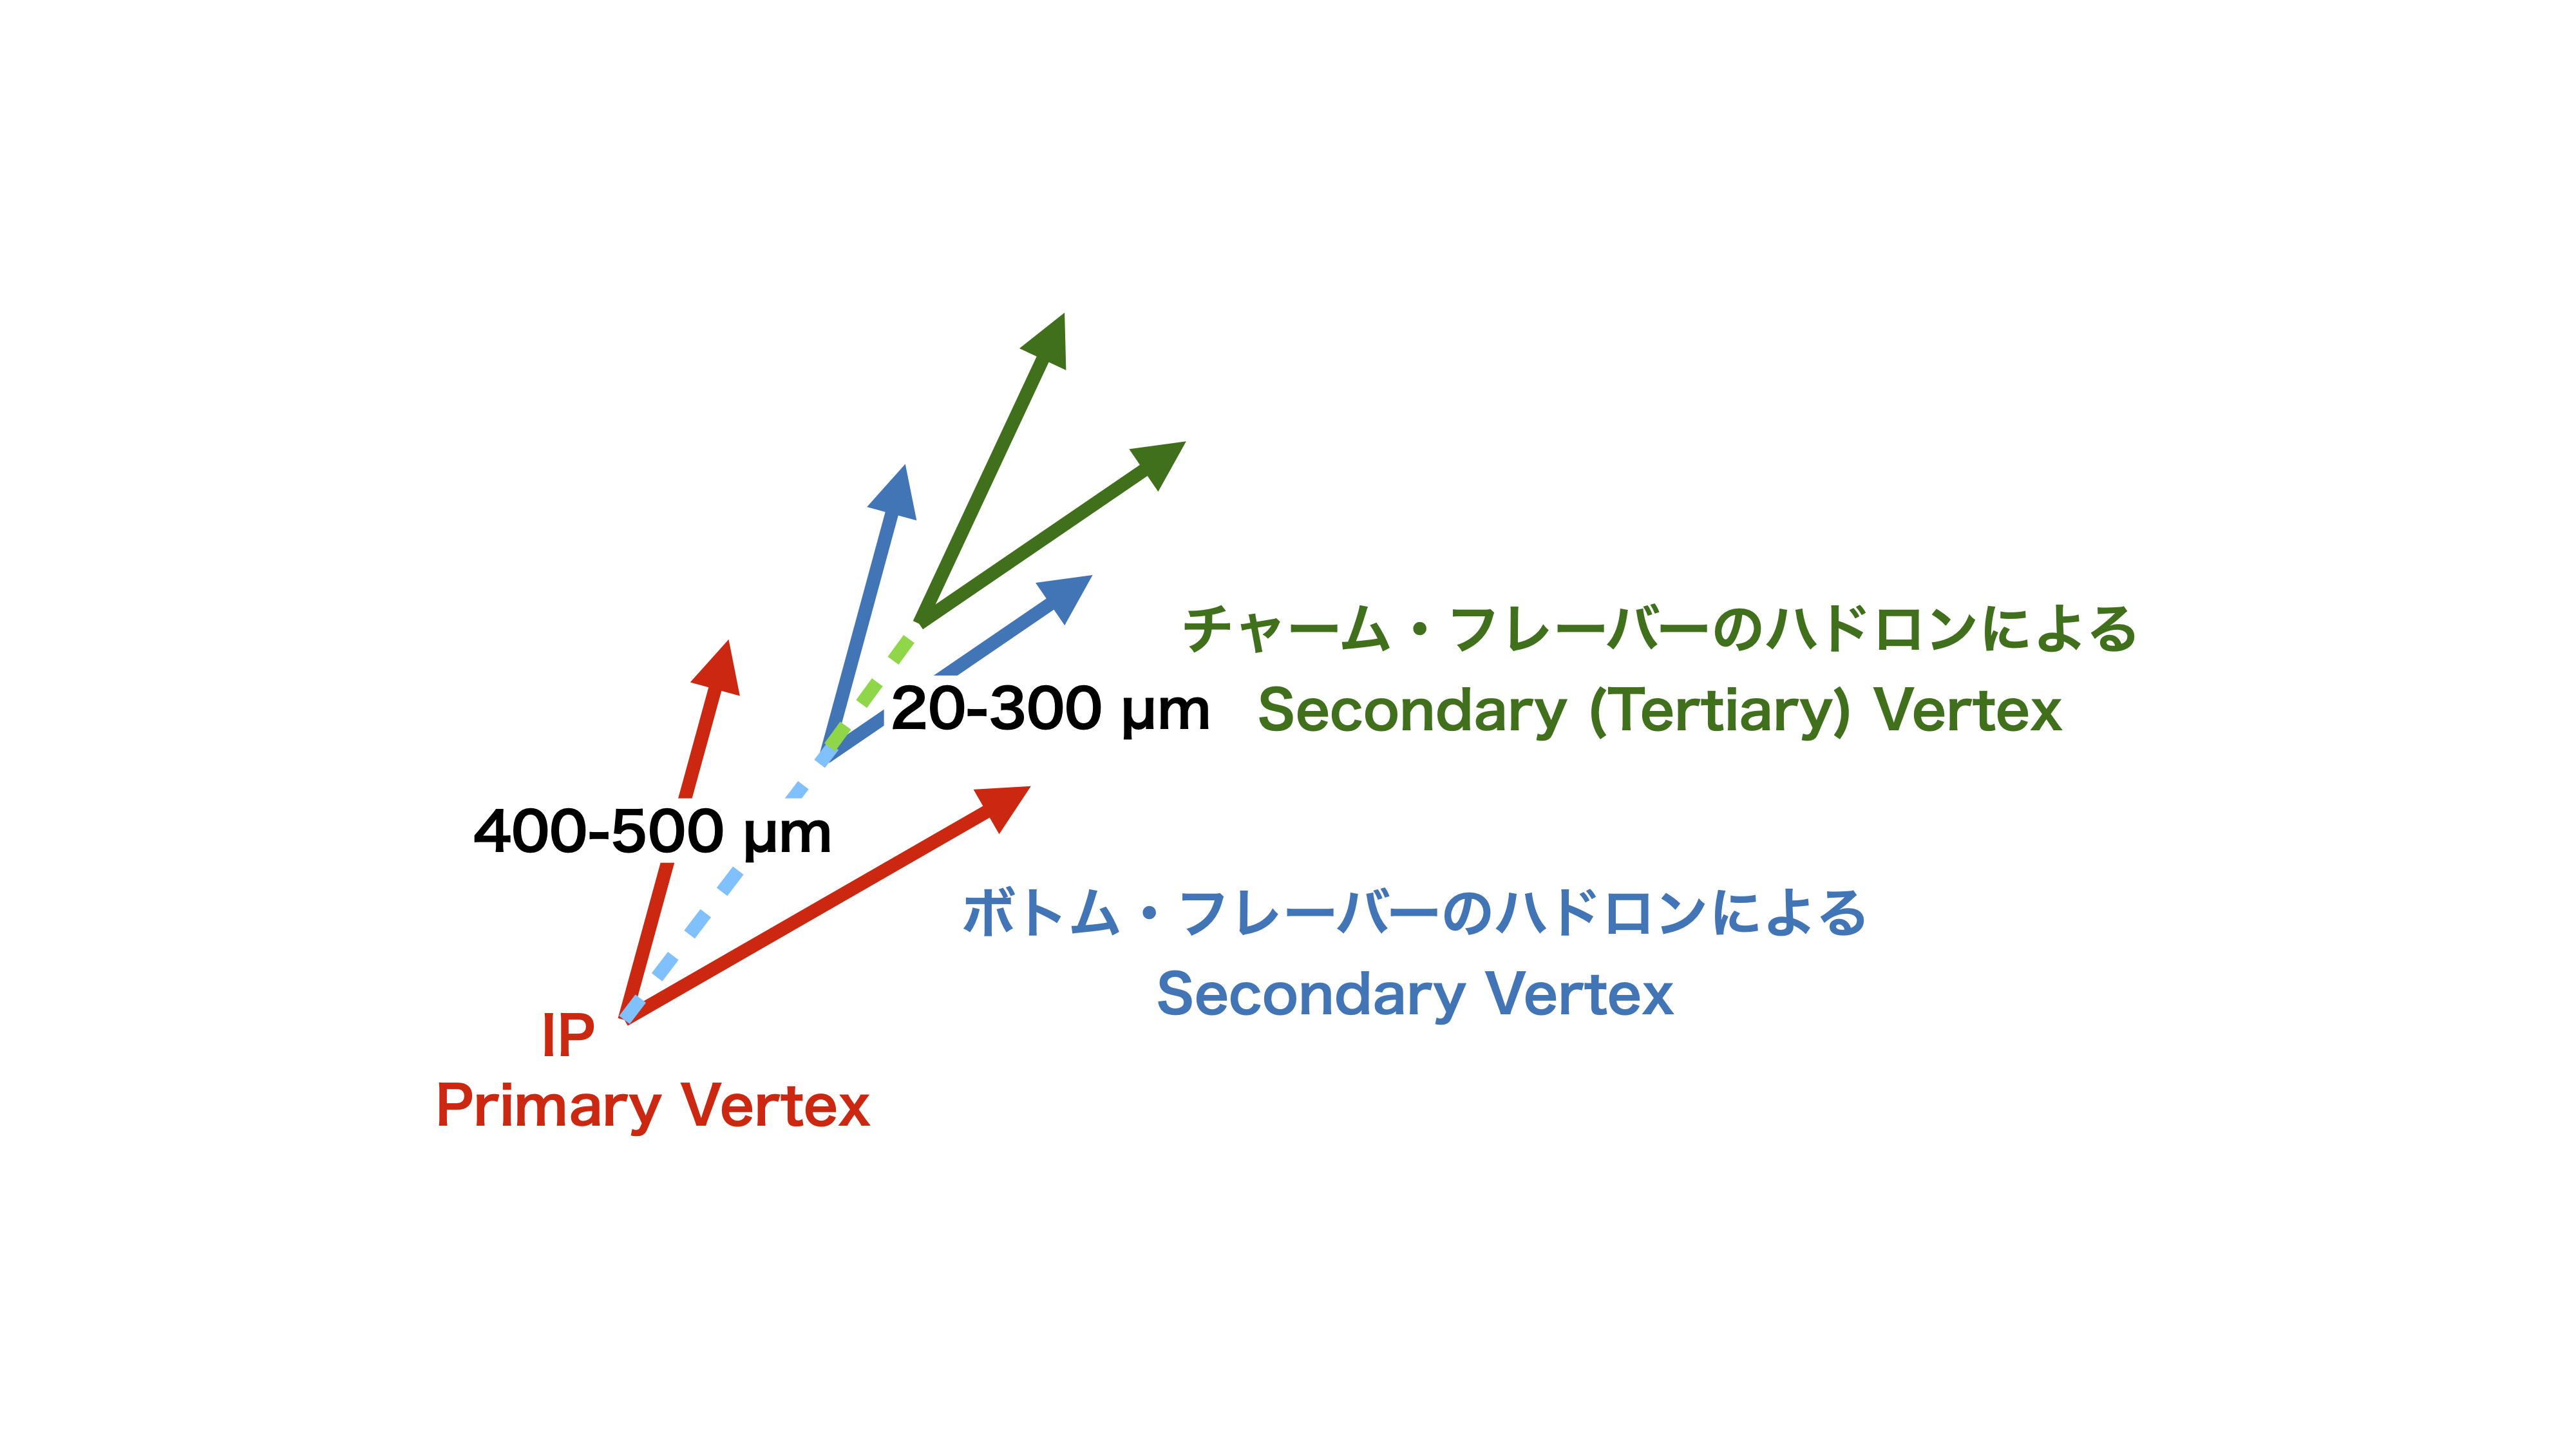
\includegraphics[trim = 200 150 200 150, width=0.9\textwidth, clip]{Figure/3Networks/3-1-1-1FinalStateBB.png}
 \caption{終状態$\rm b\bar{b}$での崩壊点の例}
 \label{3-1-1-1FinalStateBB}
\end{figure}

また、これら以外の崩壊点としてタウ粒子の崩壊やストレンジ・フレーバーのハドロンの崩壊、光子変換によるものを考えることができる。
これらの崩壊点はSecondary VertexやTertiary Vertexと比較して、衝突点から遠い位置で生じる。
そのような崩壊点を以後Othersと呼ぶ。
図\ref{3-1-1-2TracksandVertices}は一つの事象に含まれる飛跡の本数と崩壊点の個数である。
これらの粒子識別はMC情報を利用した。
ここでは飛跡の本数は親粒子のフレーバーのみ考慮し、同フレーバーの親粒子の違いは区別していない。
したがってSecondary Vertexについては、一つの崩壊点ではなく複数の崩壊点の飛跡が含まれている。
また、崩壊点の個数では親粒子を全て区別している。
したがって典型的な崩壊点の個数は終状態が$\rm c\bar{c}$の場合、Primary Vertex、チャーム・フレーバーのSecondary Vertexが2つ、Othersの$3-5$個である。
終状態が$\rm b\bar{b}$の場合はPrimary Vertex、ボトム・フレーバーのSecondary Vertexが2つ、チャーム・フレーバーのTertiary Vertexが2つ、Othersの$5-7$個である。

\begin{figure}[htbp]
 \centering
 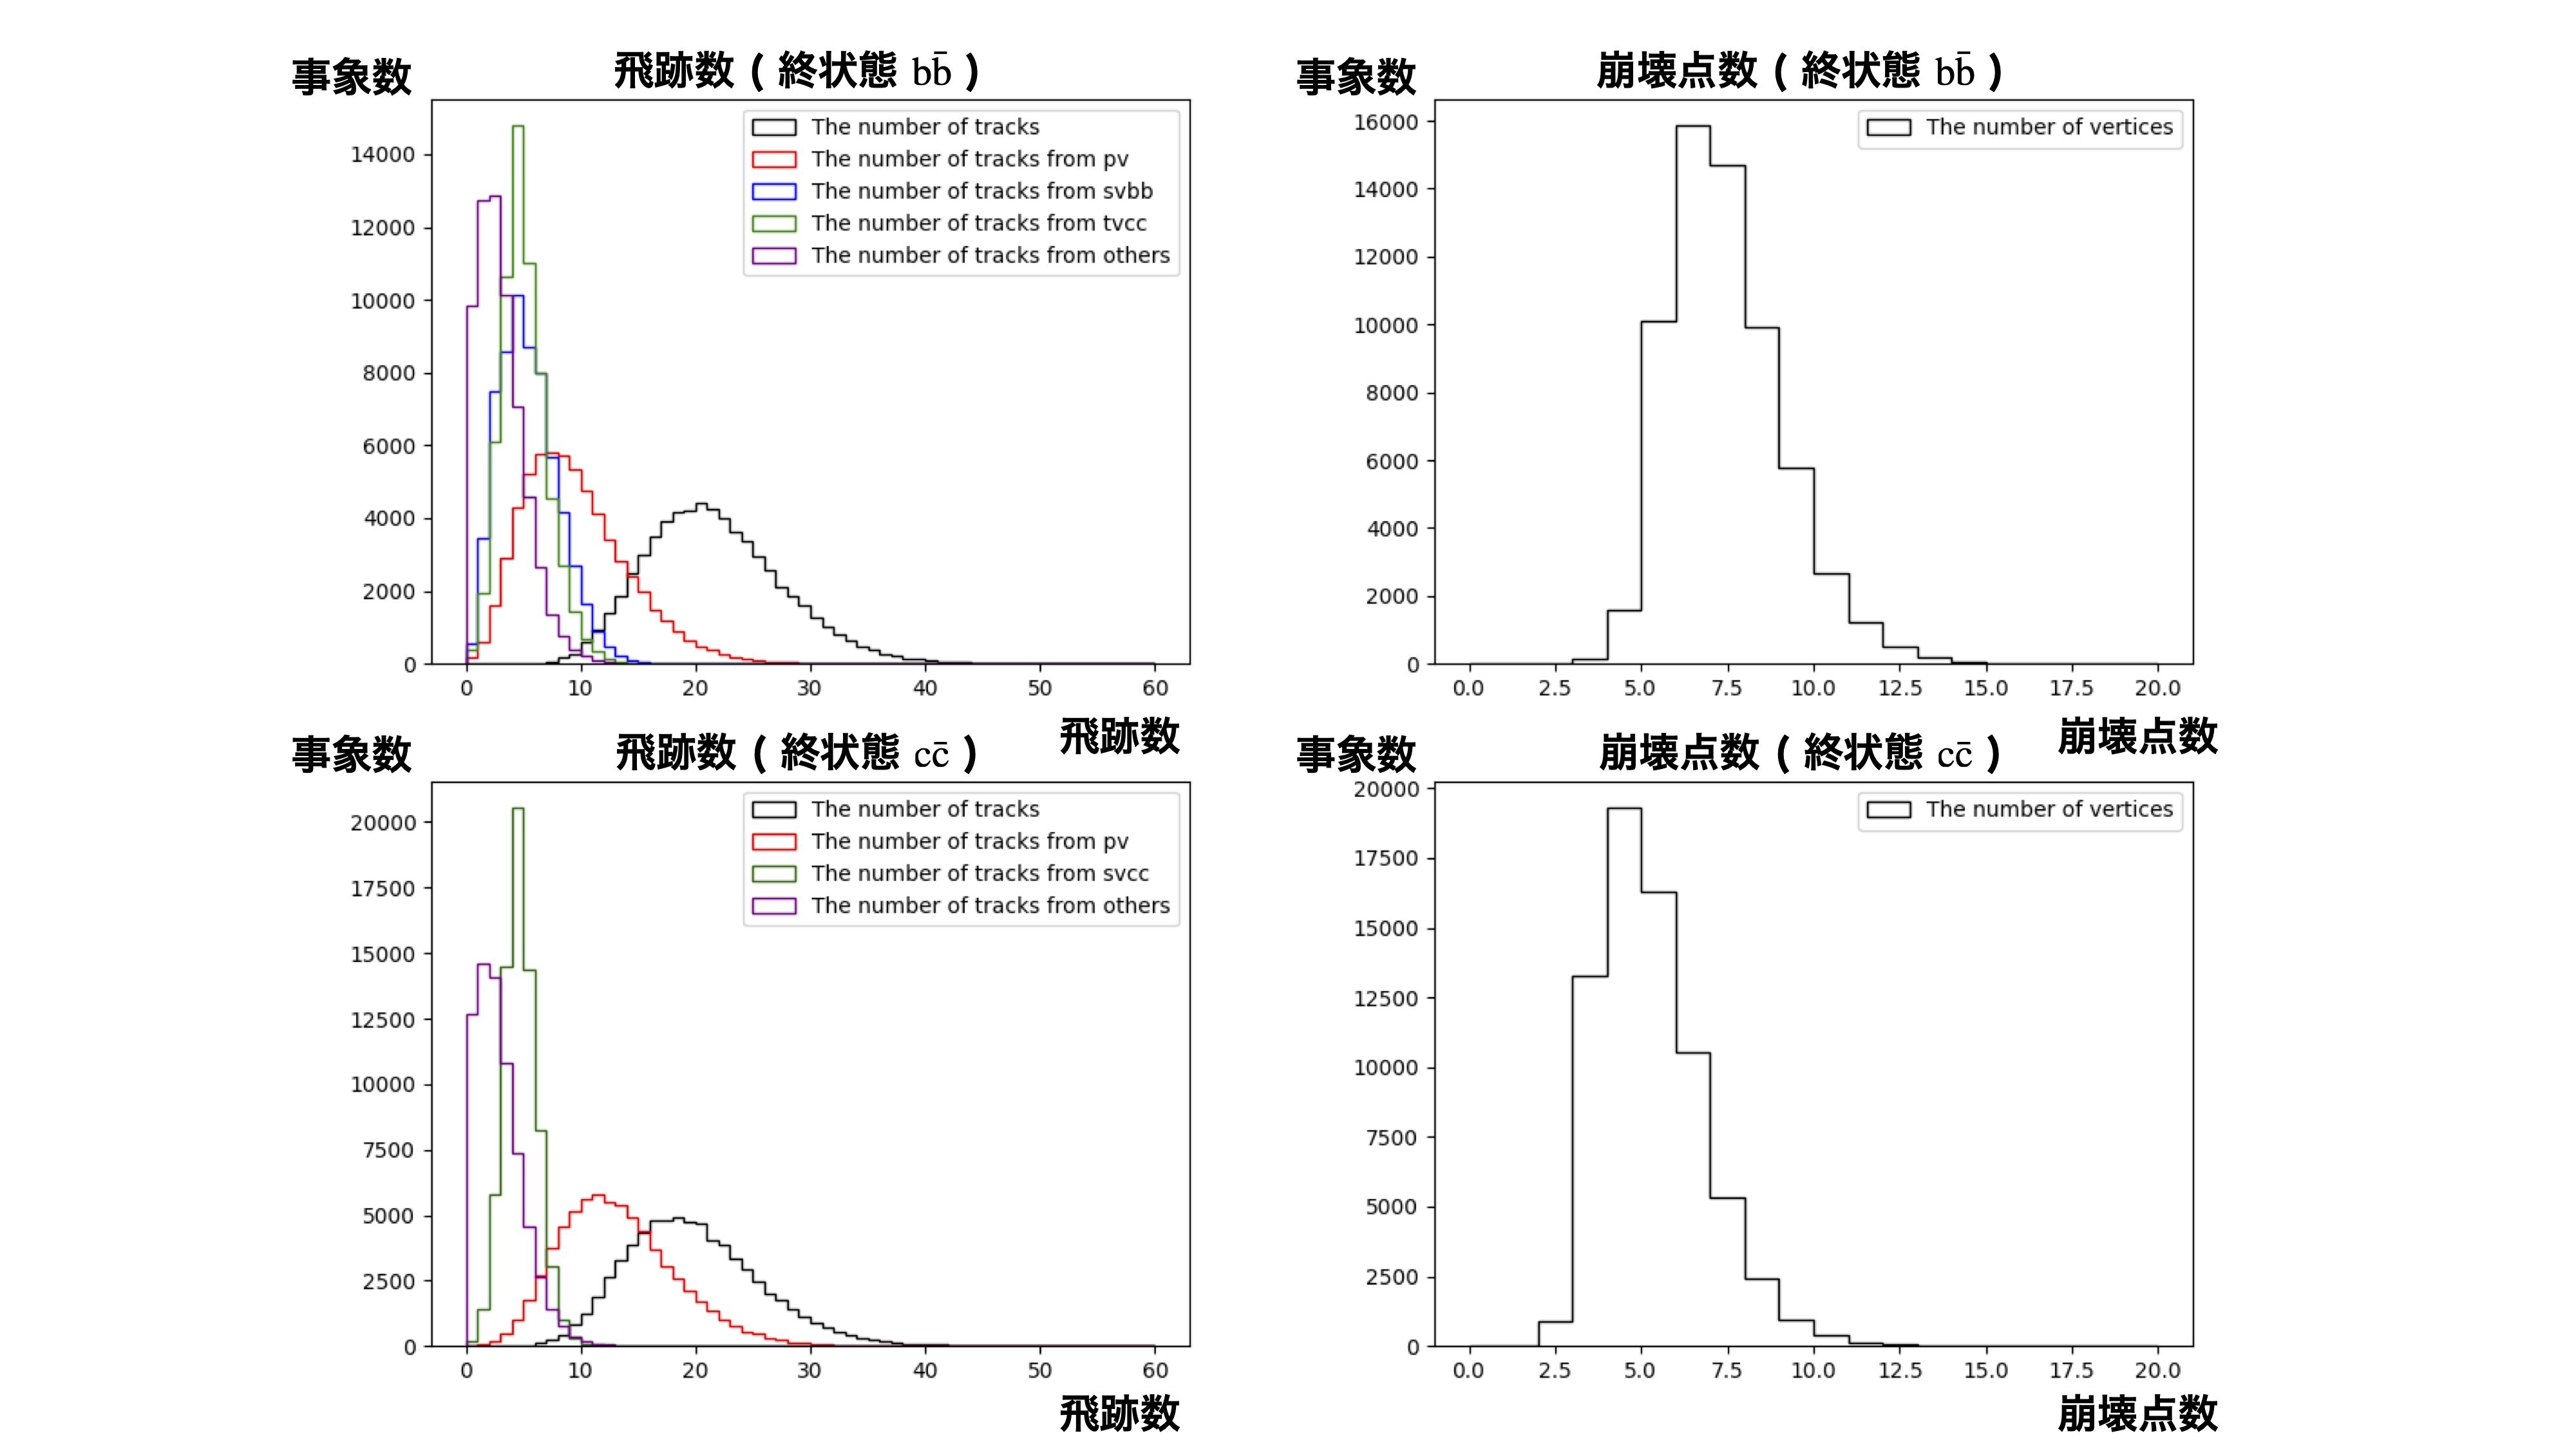
\includegraphics[trim = 150 0 150 0, width=1.0\textwidth, clip]{Figure/3Networks/3-1-1-2TracksandVertices.png}
 \caption{事象に含まれる飛跡の本数と崩壊点の個数}
 \label{3-1-1-2TracksandVertices}
\end{figure}

図\ref{3-1-1-2TracksandVertices}から分かるように、同フレーバーの親粒子の違いを区別しない場合のSecondary Vertexの飛跡の数は$5$本程度である。
したがって一つのSecondary Vertexに含まれる飛跡の数は$2-3$本程度であり、崩壊点検出ではこれらPrimary Vertexや個々の親粒子によって生じたSecondary Vertexを見分ける必要がある。


%%%%%%%%%%%%%%%%%%%%%%%%%%%%%%%%%%%%%%%%%%%%%%%%%%%%%%%%%%%%%%%%%%%%%%%%
\subsection{飛跡の情報と前処理} \label{Net:Data:TrackInformationandPreprocessing}

飛跡の情報として、図\ref{3-1-2-1TrackParameters}のような位置や運動量の情報を含んだトラック・パラメータ$5$個 ($\rm d_0$, $\rm z_0$, $\rm \phi$, $\rm \Omega$, $\rm \tan{\lambda}$)\cite{TrackParametersLCIO}とその共分散行列$15$個、電荷、エネルギーの計$22$個の変数を使用した。
また、加速器の座標系としてビーム衝突点を原点とし、Z軸をビーム方向にとった直交座標系・球座標系を使用する。

\begin{figure}[htbp]
 \centering
 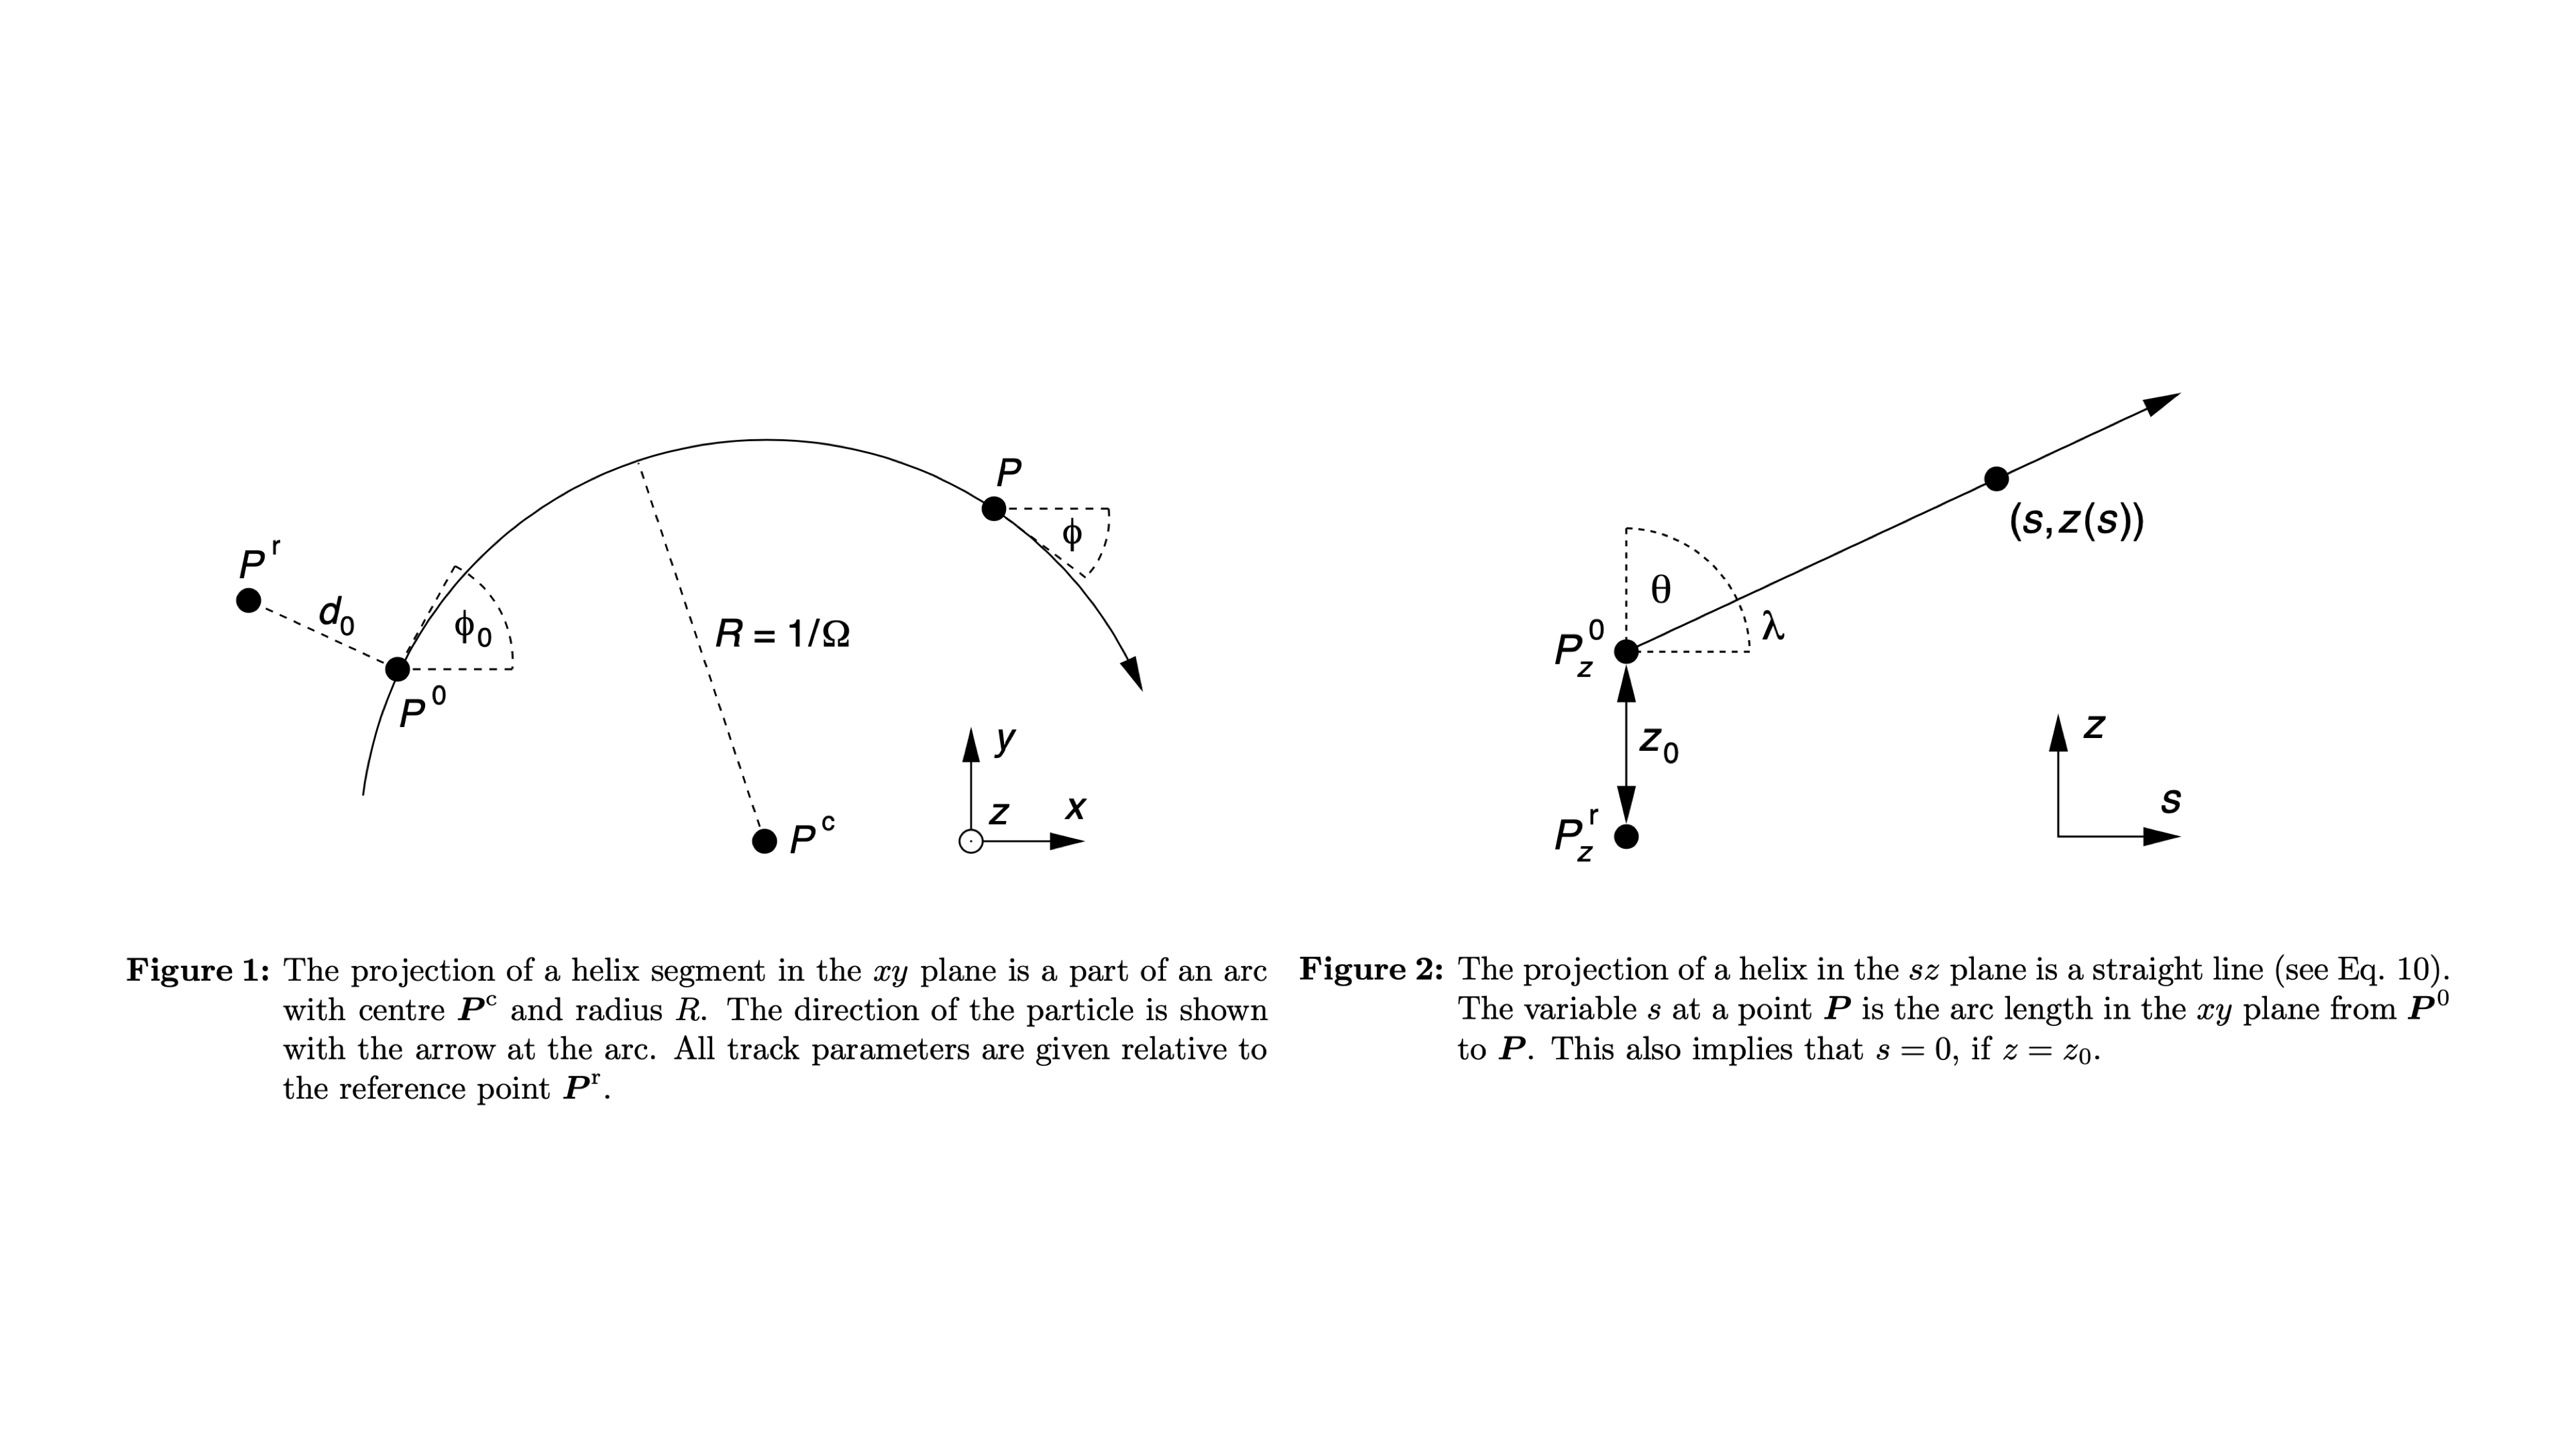
\includegraphics[trim = 50 150 50 250, width=1.0\textwidth, clip]{Figure/3Networks/3-1-2-1TrackParameters.png}
 \caption{トラック・パラメータの定義\cite{TrackParametersLCIO}}
 \label{3-1-2-1TrackParameters}
\end{figure}

深層学習の入力に使用する変数は、一般に$[-1,\ 1]$の範囲に整形した方が良いと言われている為、変数をそれぞれ以下のような$\tanh$関数や線形関数などを用いて整形した。

\begin{itemize}
 \item トラック・パラメータ\\
 ${\rm d_0} = \tanh{({\rm d_0})}$,
 ${\rm z_0} = \tanh{({\rm z_0})}$,
 ${\rm \phi} = {\rm \phi}/\pi$,
 ${\rm \Omega} = \tanh{(200\ {\rm \Omega})}$,
 ${\rm \tan{\lambda}} = \tanh{(0.3\ {\rm \tan{\lambda}})}$
 \item トラック・パラメータの共分散行列\\
 $\tanh{(8000\ (x-0.0005))}$
 \item エネルギー\\
 $\tanh{(0.5\ (x-5.0))}$
\end{itemize}

トラック・パラメータとエネルギーの整形前と整形後の分布をそれぞれ図\ref{3-1-2-2Variables}に示す。
整形後の変数の分布が$[-1,\ 1]$の範囲になっていることがわかる。

\begin{figure}[htbp]
 \centering
  %\begin{tabular}{cccc}
  \begin{minipage}{1.0\textwidth}
  \centering
   \begin{minipage}{0.48\textwidth}
    \centering
    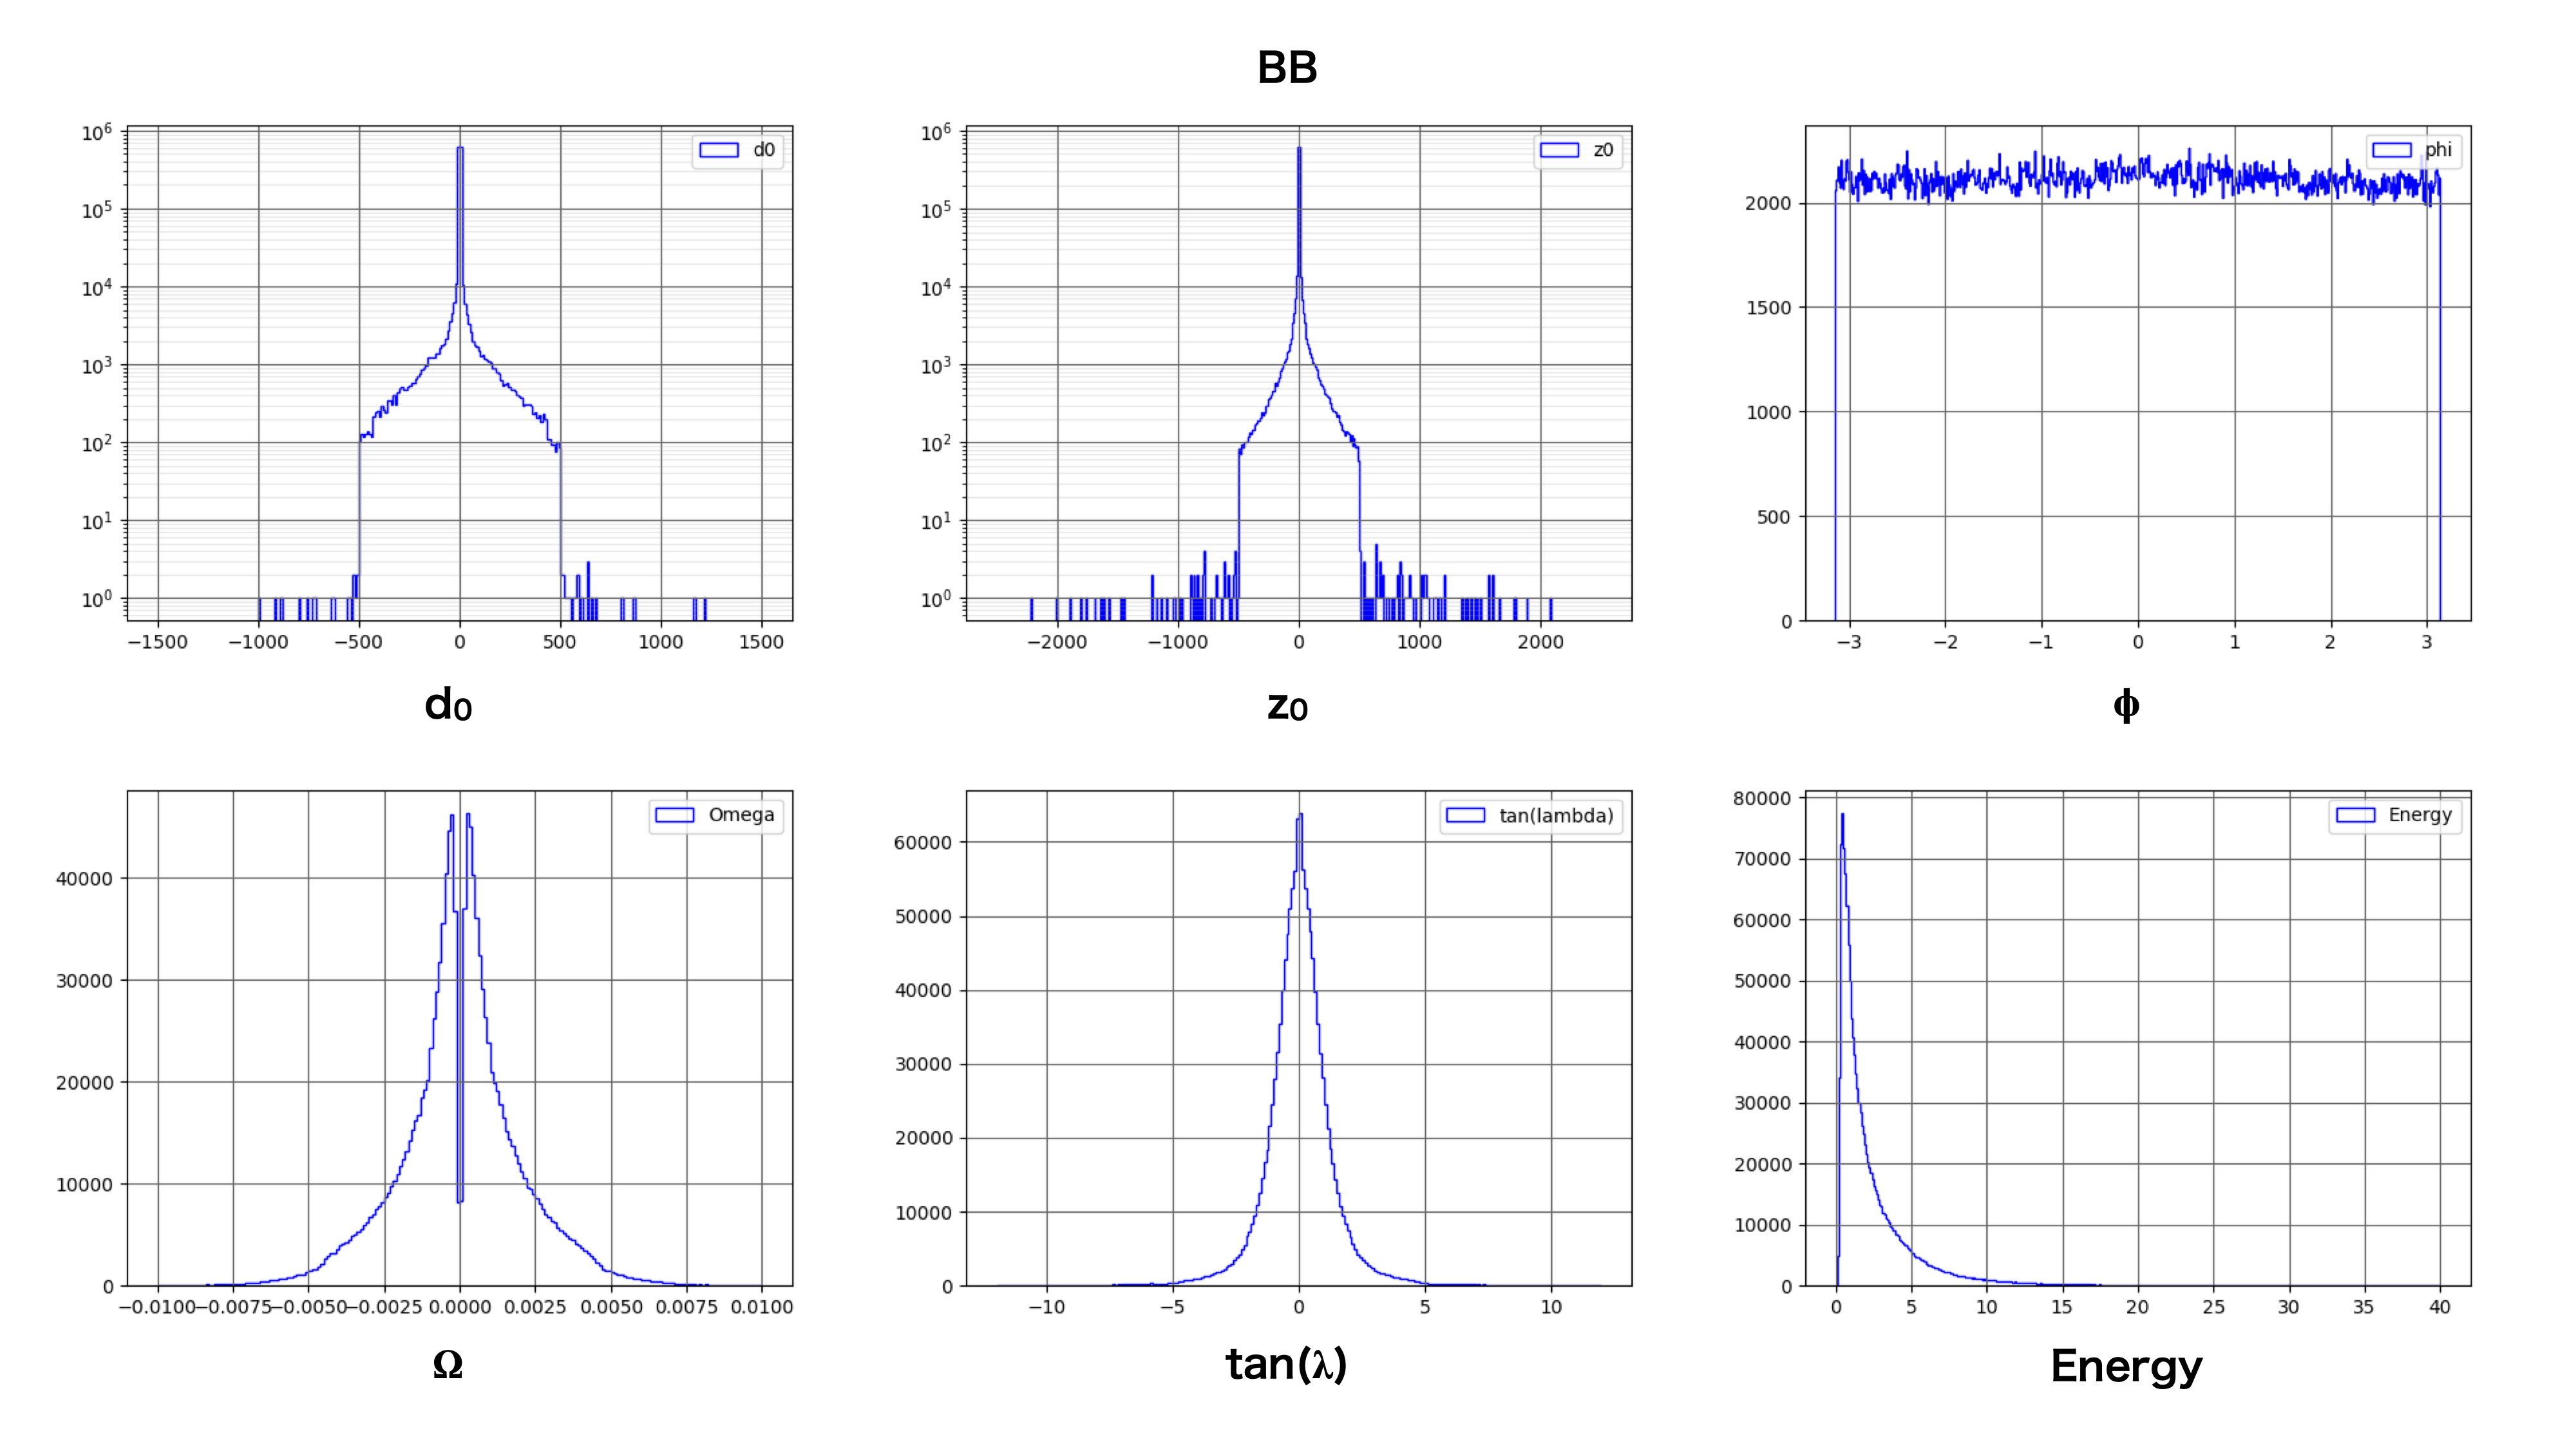
\includegraphics[width=1.0\textwidth, clip]{Figure/3Networks/3-1-2-2OriginalVariablesBB.png}
    \subcaption{終状態$\rm b\bar{b}$での変換前の変数の分布}
    \label{3-1-2-2OriginalVariablesBB}
   \end{minipage}
   \begin{minipage}{0.48\textwidth}
   \centering
    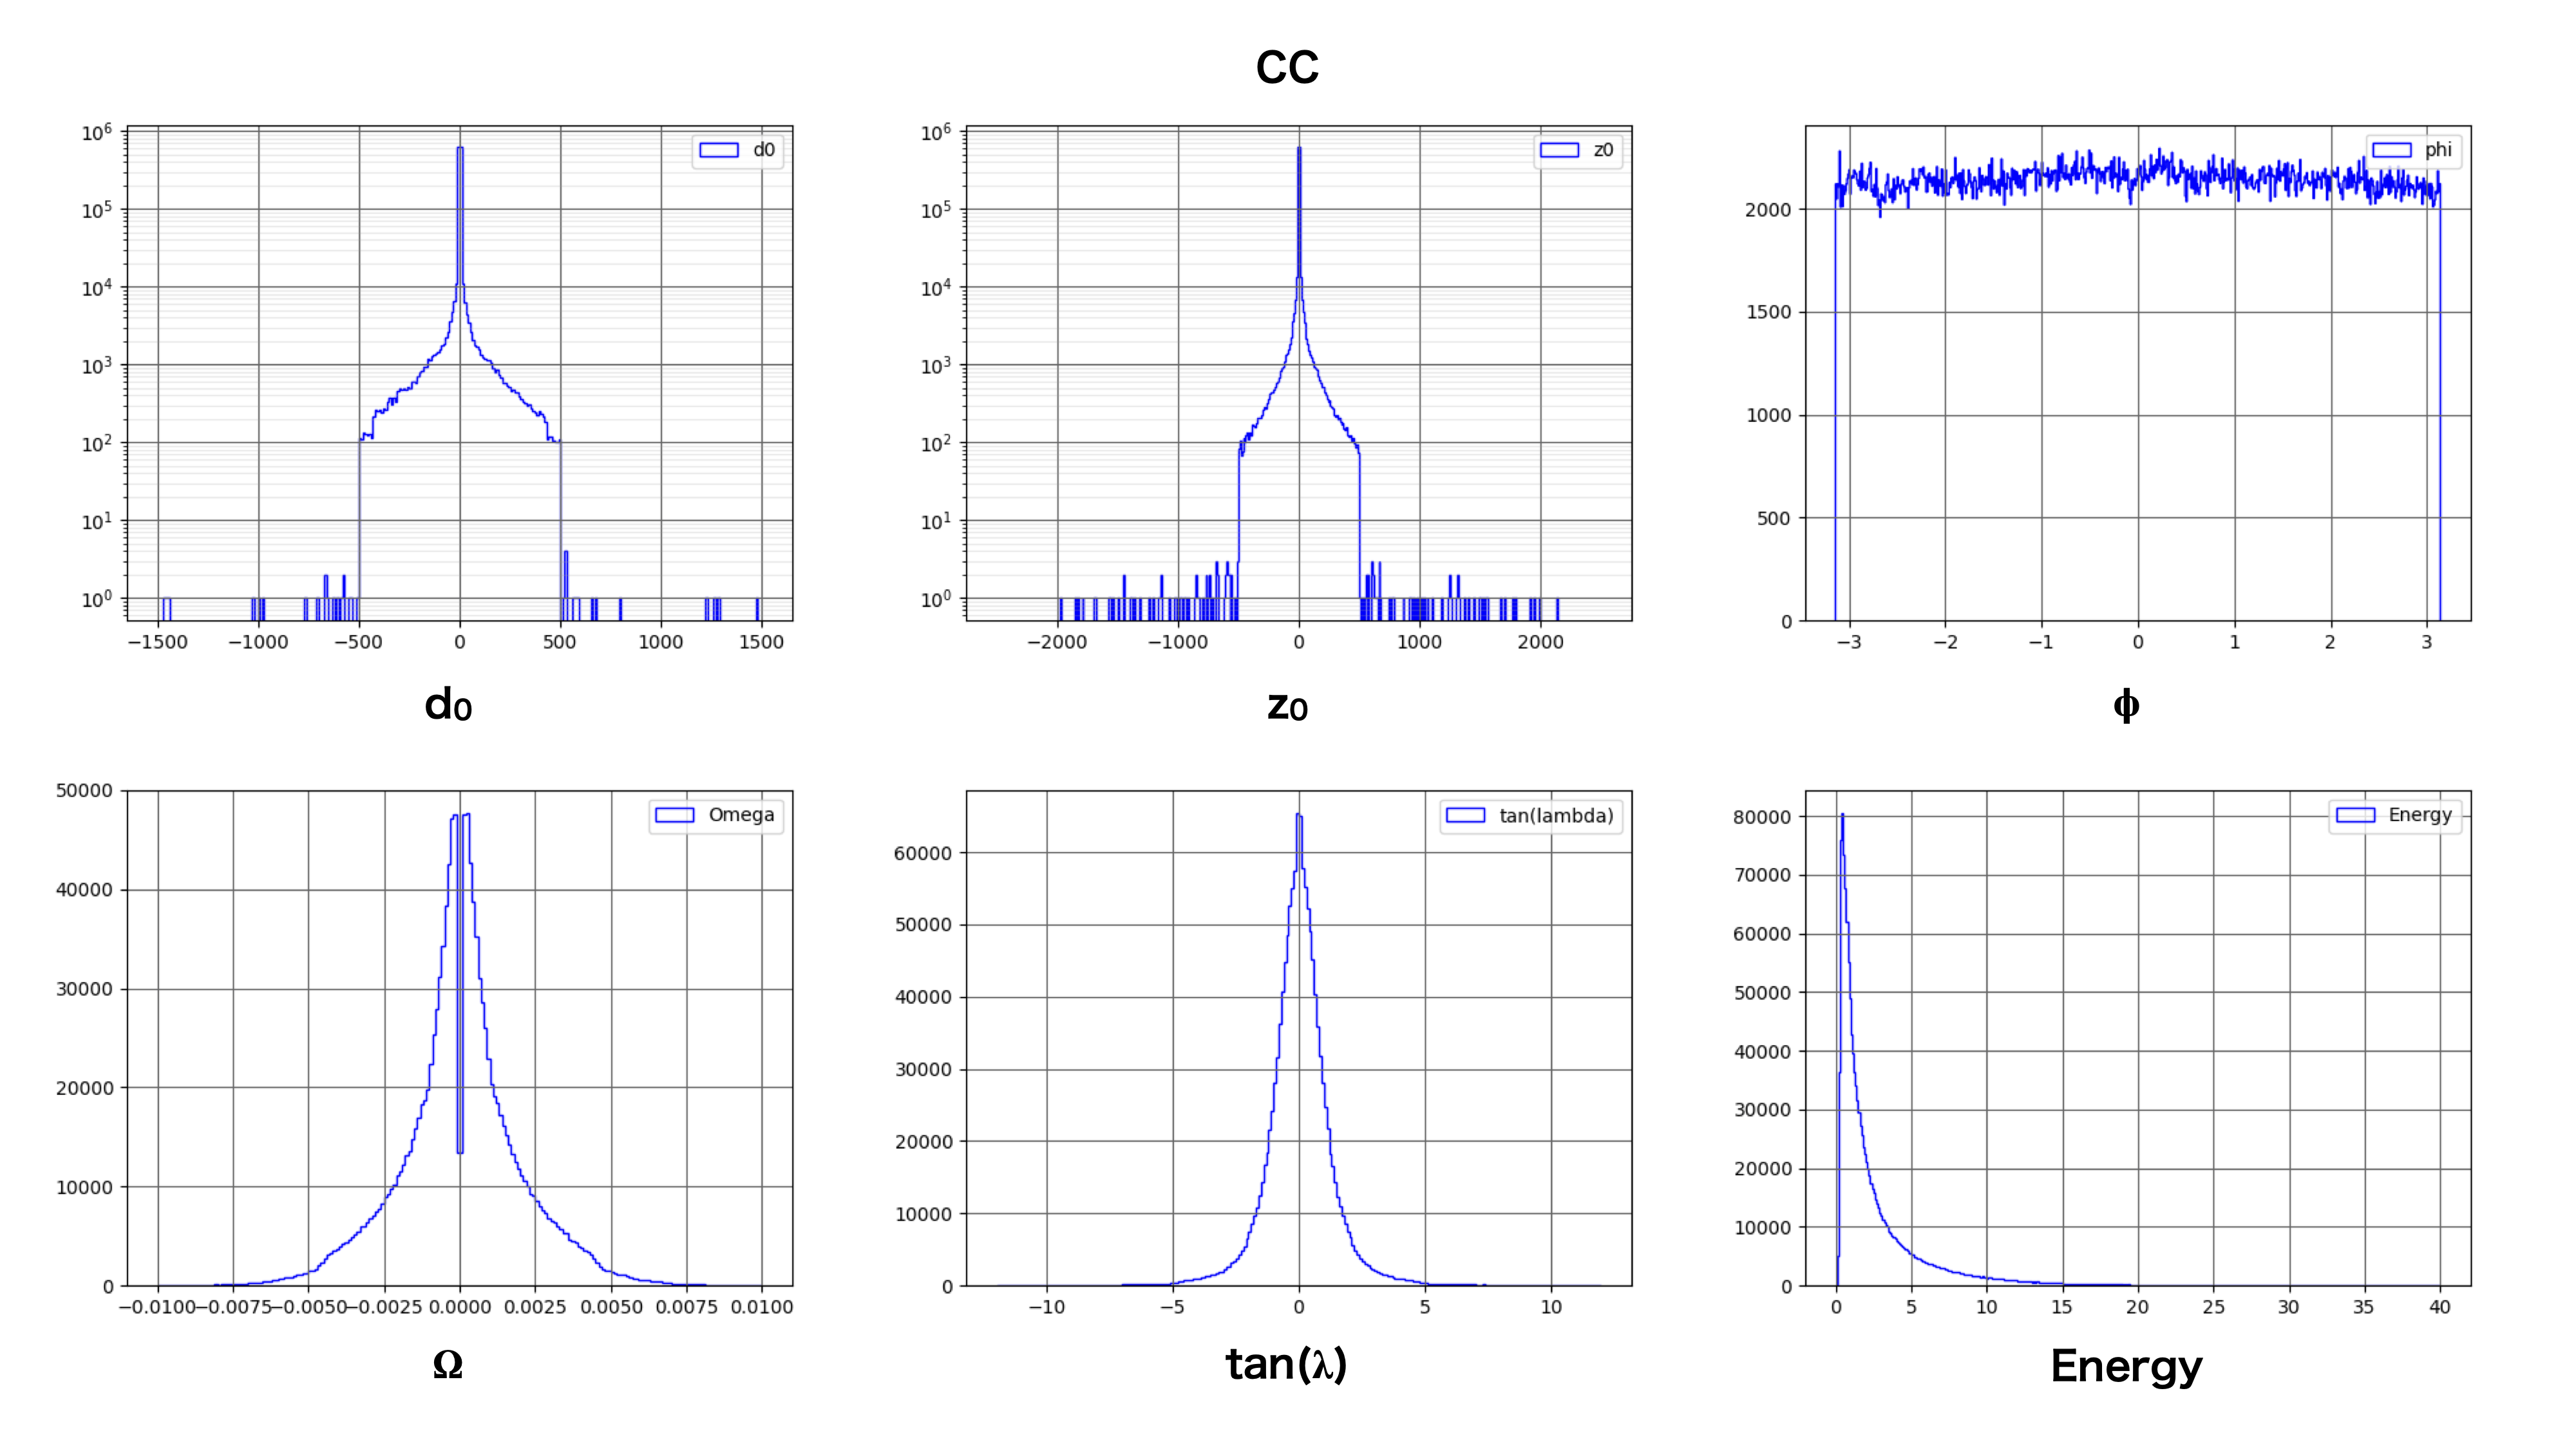
\includegraphics[width=1.0\textwidth, clip]{Figure/3Networks/3-1-2-2OriginalVariablesCC.png}
    \subcaption{終状態$\rm c\bar{c}$での変換前の変数の分布}
    \label{3-1-2-2OriginalVariablesCC}
   \end{minipage}
  \end{minipage}
  
  \begin{minipage}{1.0\textwidth}
  \centering
   \begin{minipage}{0.48\textwidth}
   \centering
    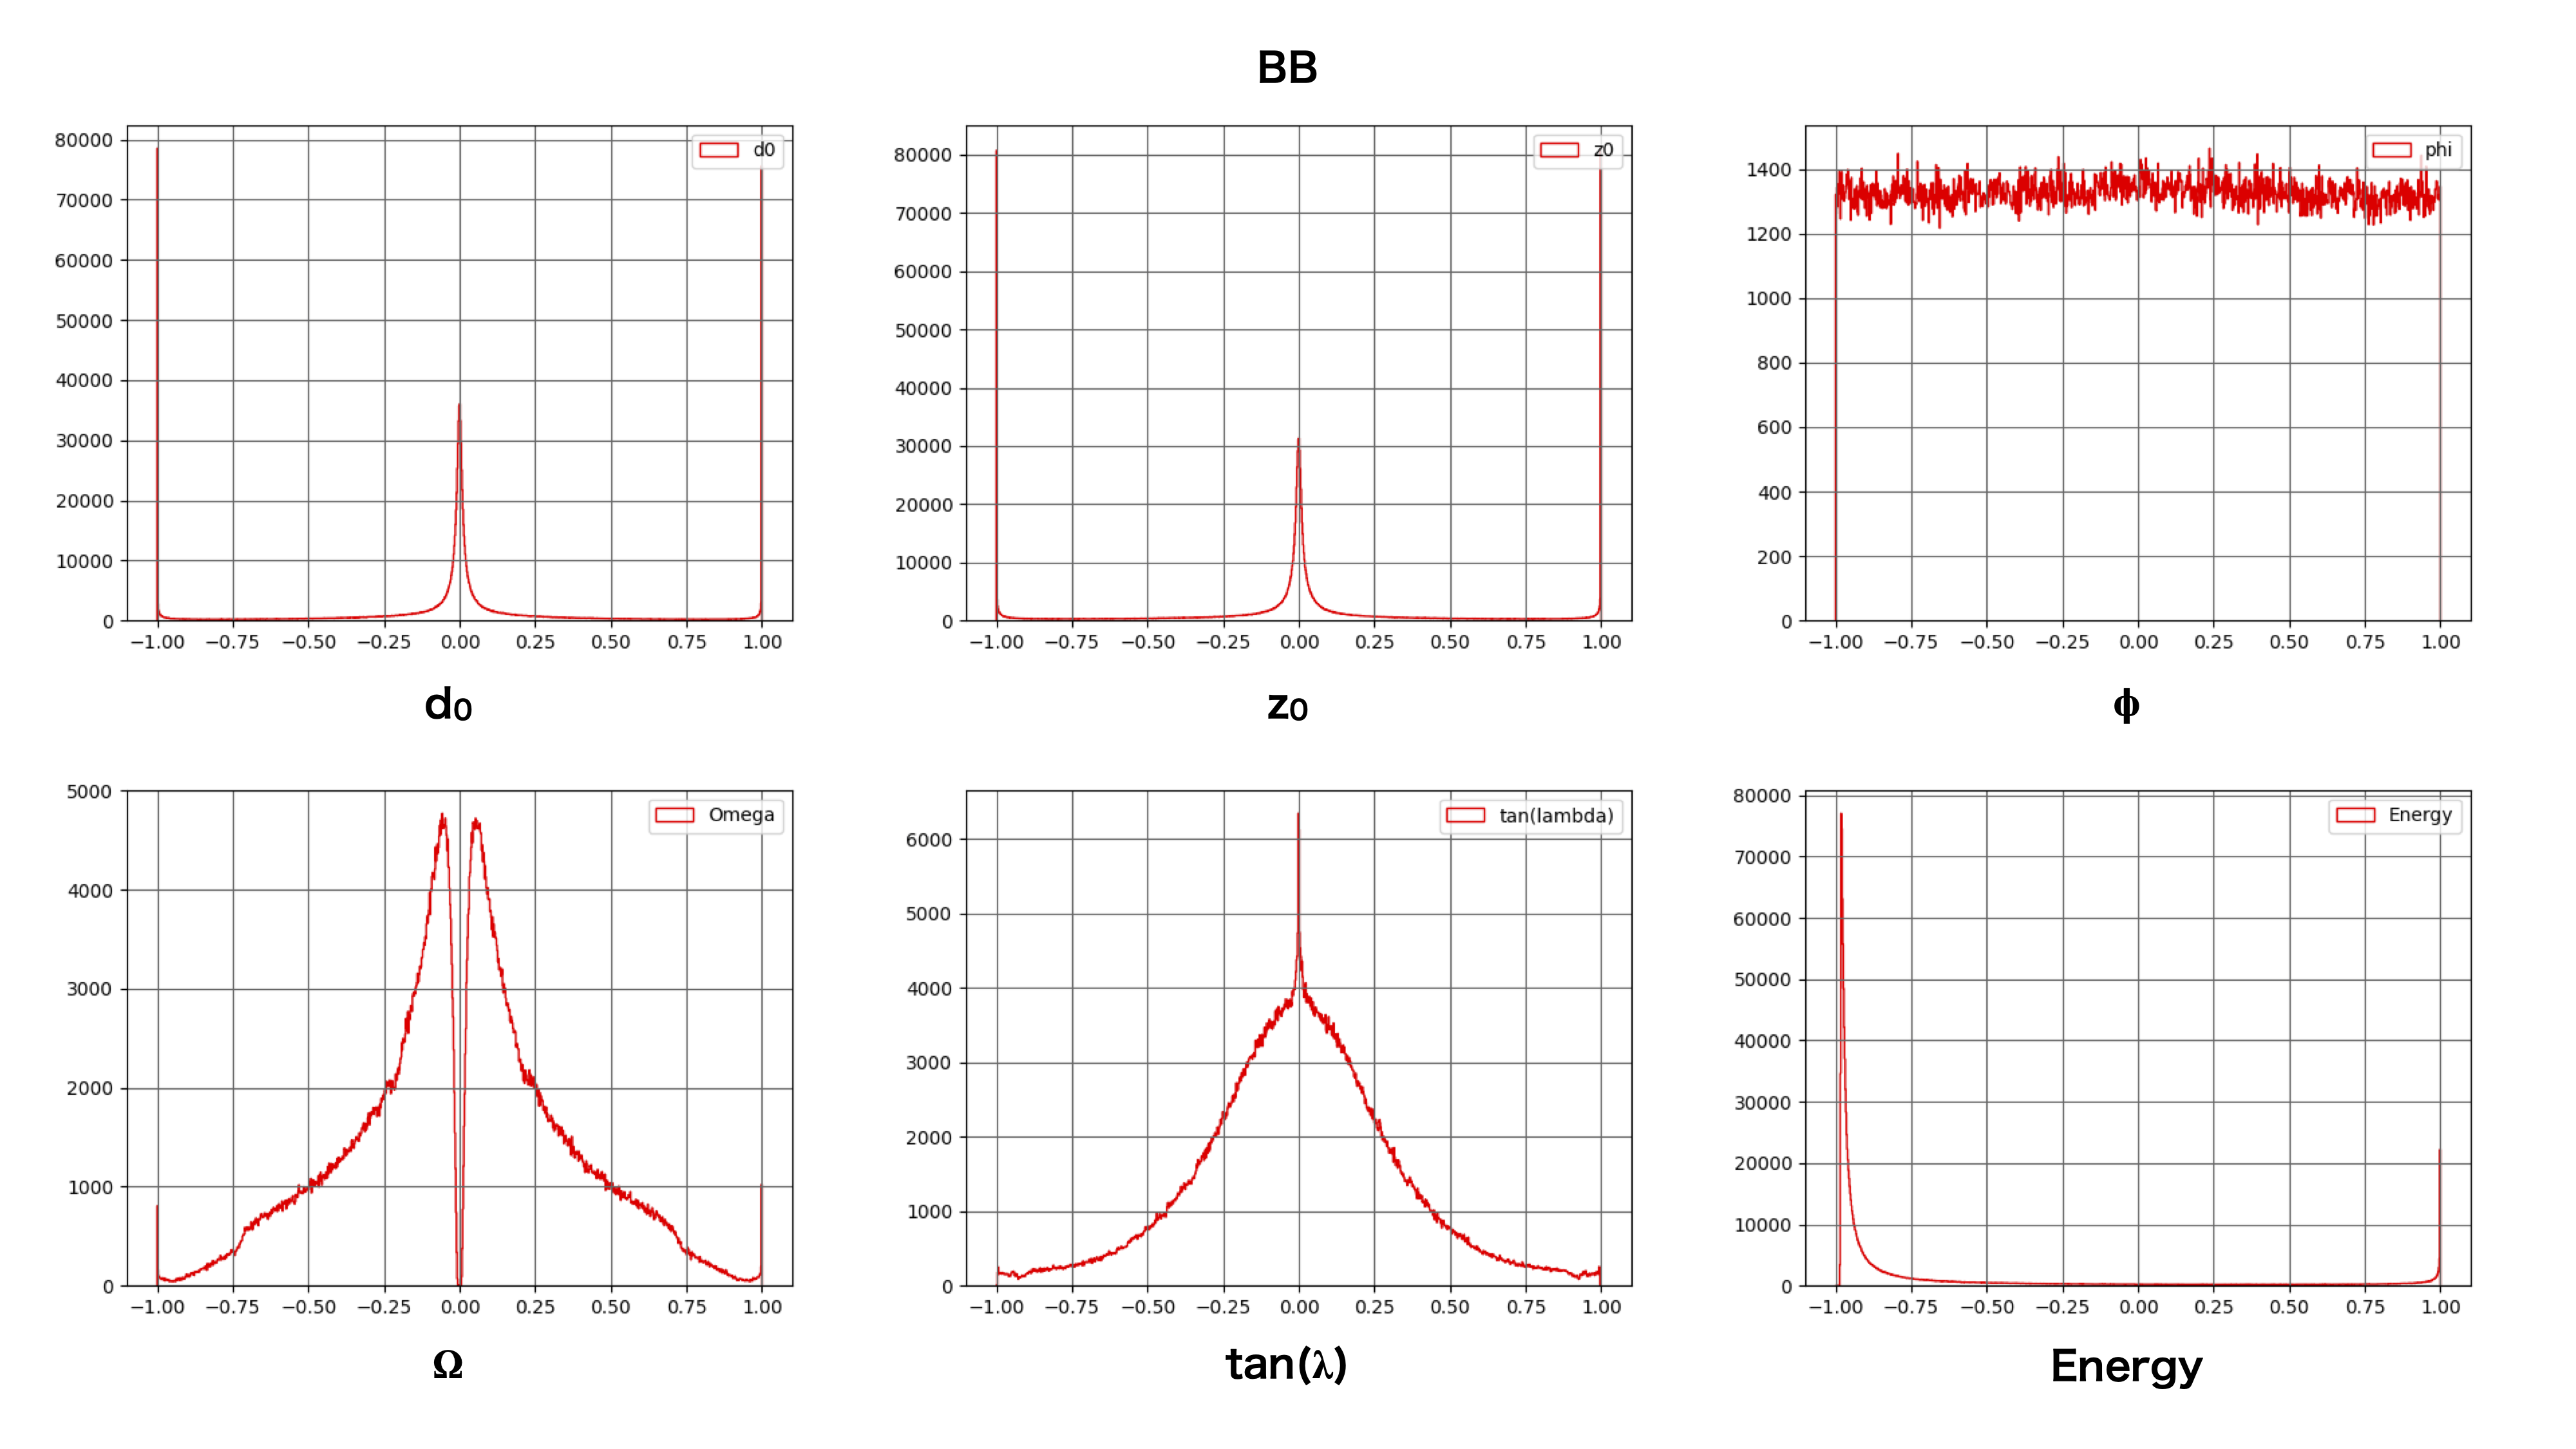
\includegraphics[width=1.0\textwidth, clip]{Figure/3Networks/3-1-2-2ReshapedVariablesBB.png}
    \subcaption{終状態$\rm b\bar{b}$での変換後の変数の分布}
    \label{3-1-2-2ReshapedVariablesBB}
   \end{minipage}
   \begin{minipage}{0.48\textwidth}
   \centering
    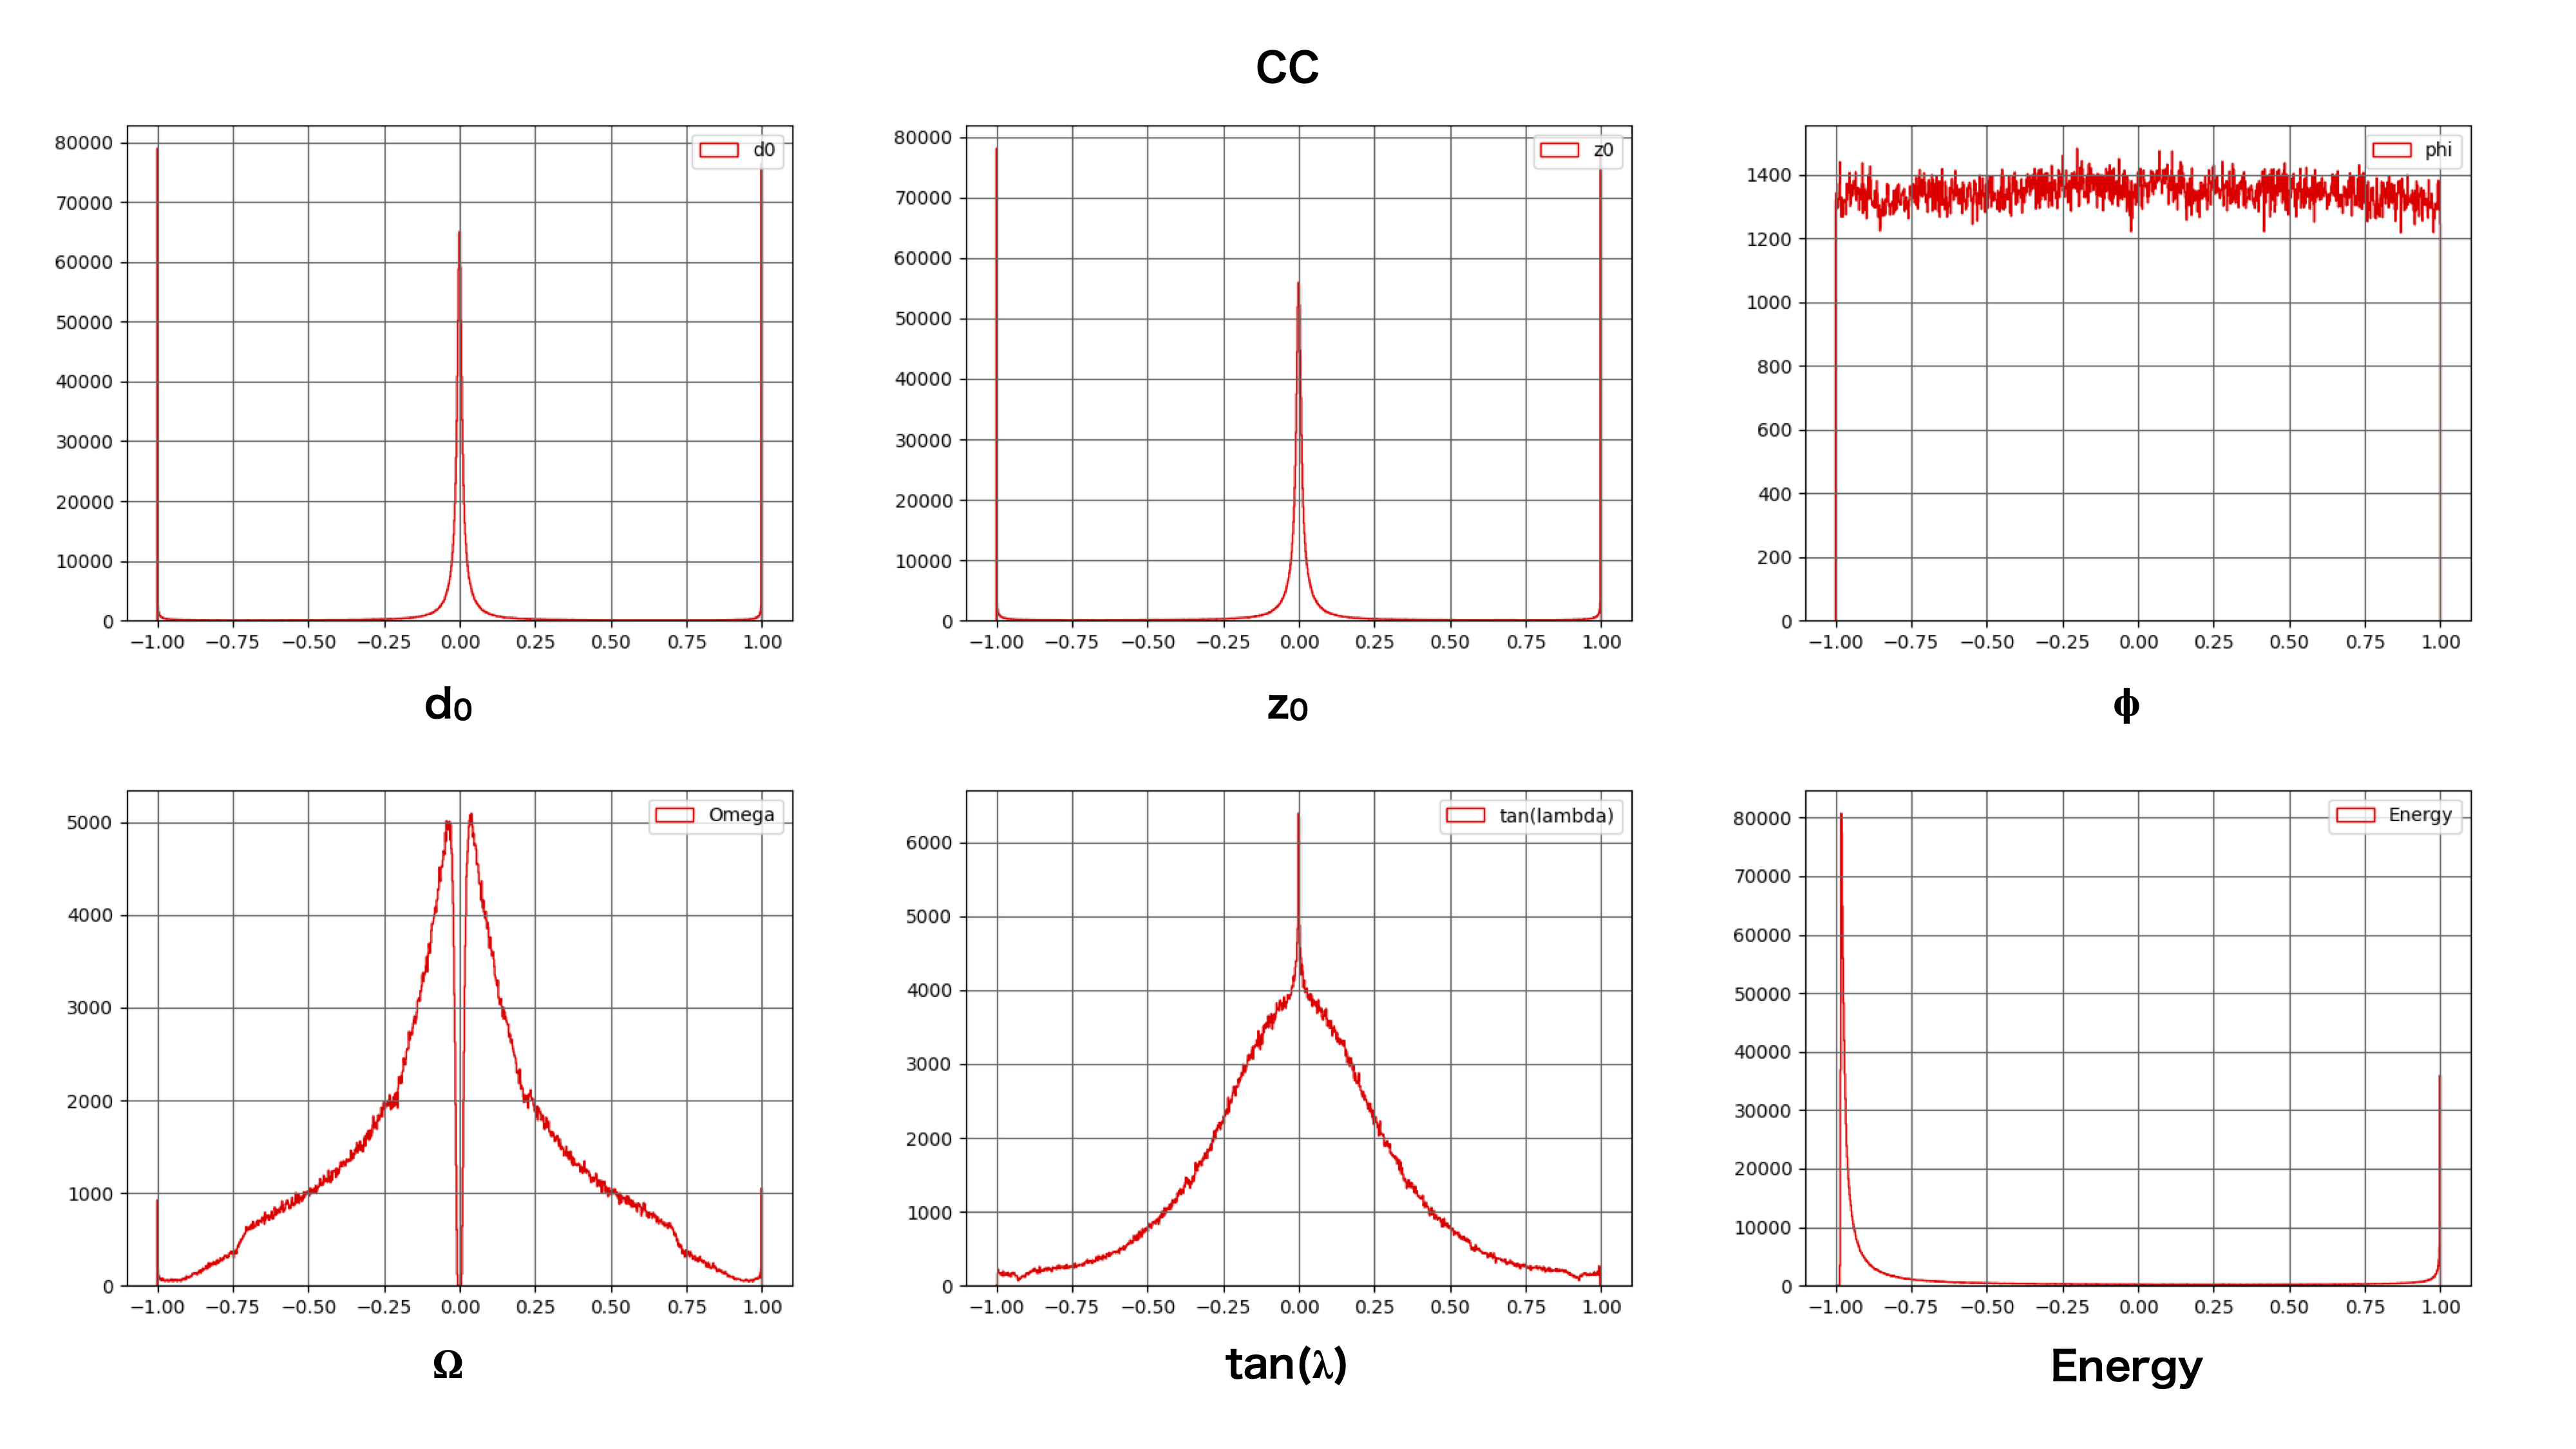
\includegraphics[width=1.0\textwidth, clip]{Figure/3Networks/3-1-2-2ReshapedVariablesCC.png}
    \subcaption{終状態$\rm c\bar{c}$での変換後の変数の分布}
    \label{3-1-2-2ReshapedVariablesCC}
   \end{minipage}
   \end{minipage}
  \caption{変数の分布の例}
  \label{3-1-2-2Variables}
 %\end{tabular}
\end{figure}

また、LCFIPlusのフィッティングで得られる$\chi^2$や崩壊点の位置についてもデータを用意した。
ここでは、事象中の二本の飛跡 (飛跡対) の組み合わせ全てについて計算を行った。
ただし、このような高次の情報を含んだ変数は基本的にはネットワークの学習に使用せず、正解ラベルの一つとして使用した。
LCFIPlusによって予想される崩壊点の位置について、ビーム衝突点からの距離を図\ref{3-1-2-3VertexPositions}に示す。
図\ref{3-1-2-3VertexPositions}のグラフは両対数グラフとして表現している為、衝突点からの距離$10^{-2}\ \mathrm{mm}$から$10^{3}\ \mathrm{mm}$のプロットとなっており、衝突点は含んでいない。
Primary VertexとSecondary Vertexの衝突点からの距離は大きく異なっているが、各フレーバーのSecondary Vertexの衝突点からの距離は殆ど離れていないことが分かる。
また、終状態$\rm c\bar{c}$と終状態$\rm b\bar{b}$では$\rm b \to c$の崩壊過程を辿らない為、チャーム・フレーバーの崩壊点の位置が少し異なっている。
Othersは衝突点付近では殆ど起こらず、他の崩壊点と比較して遠い位置で崩壊している。

\begin{figure}[htbp]
 \centering
 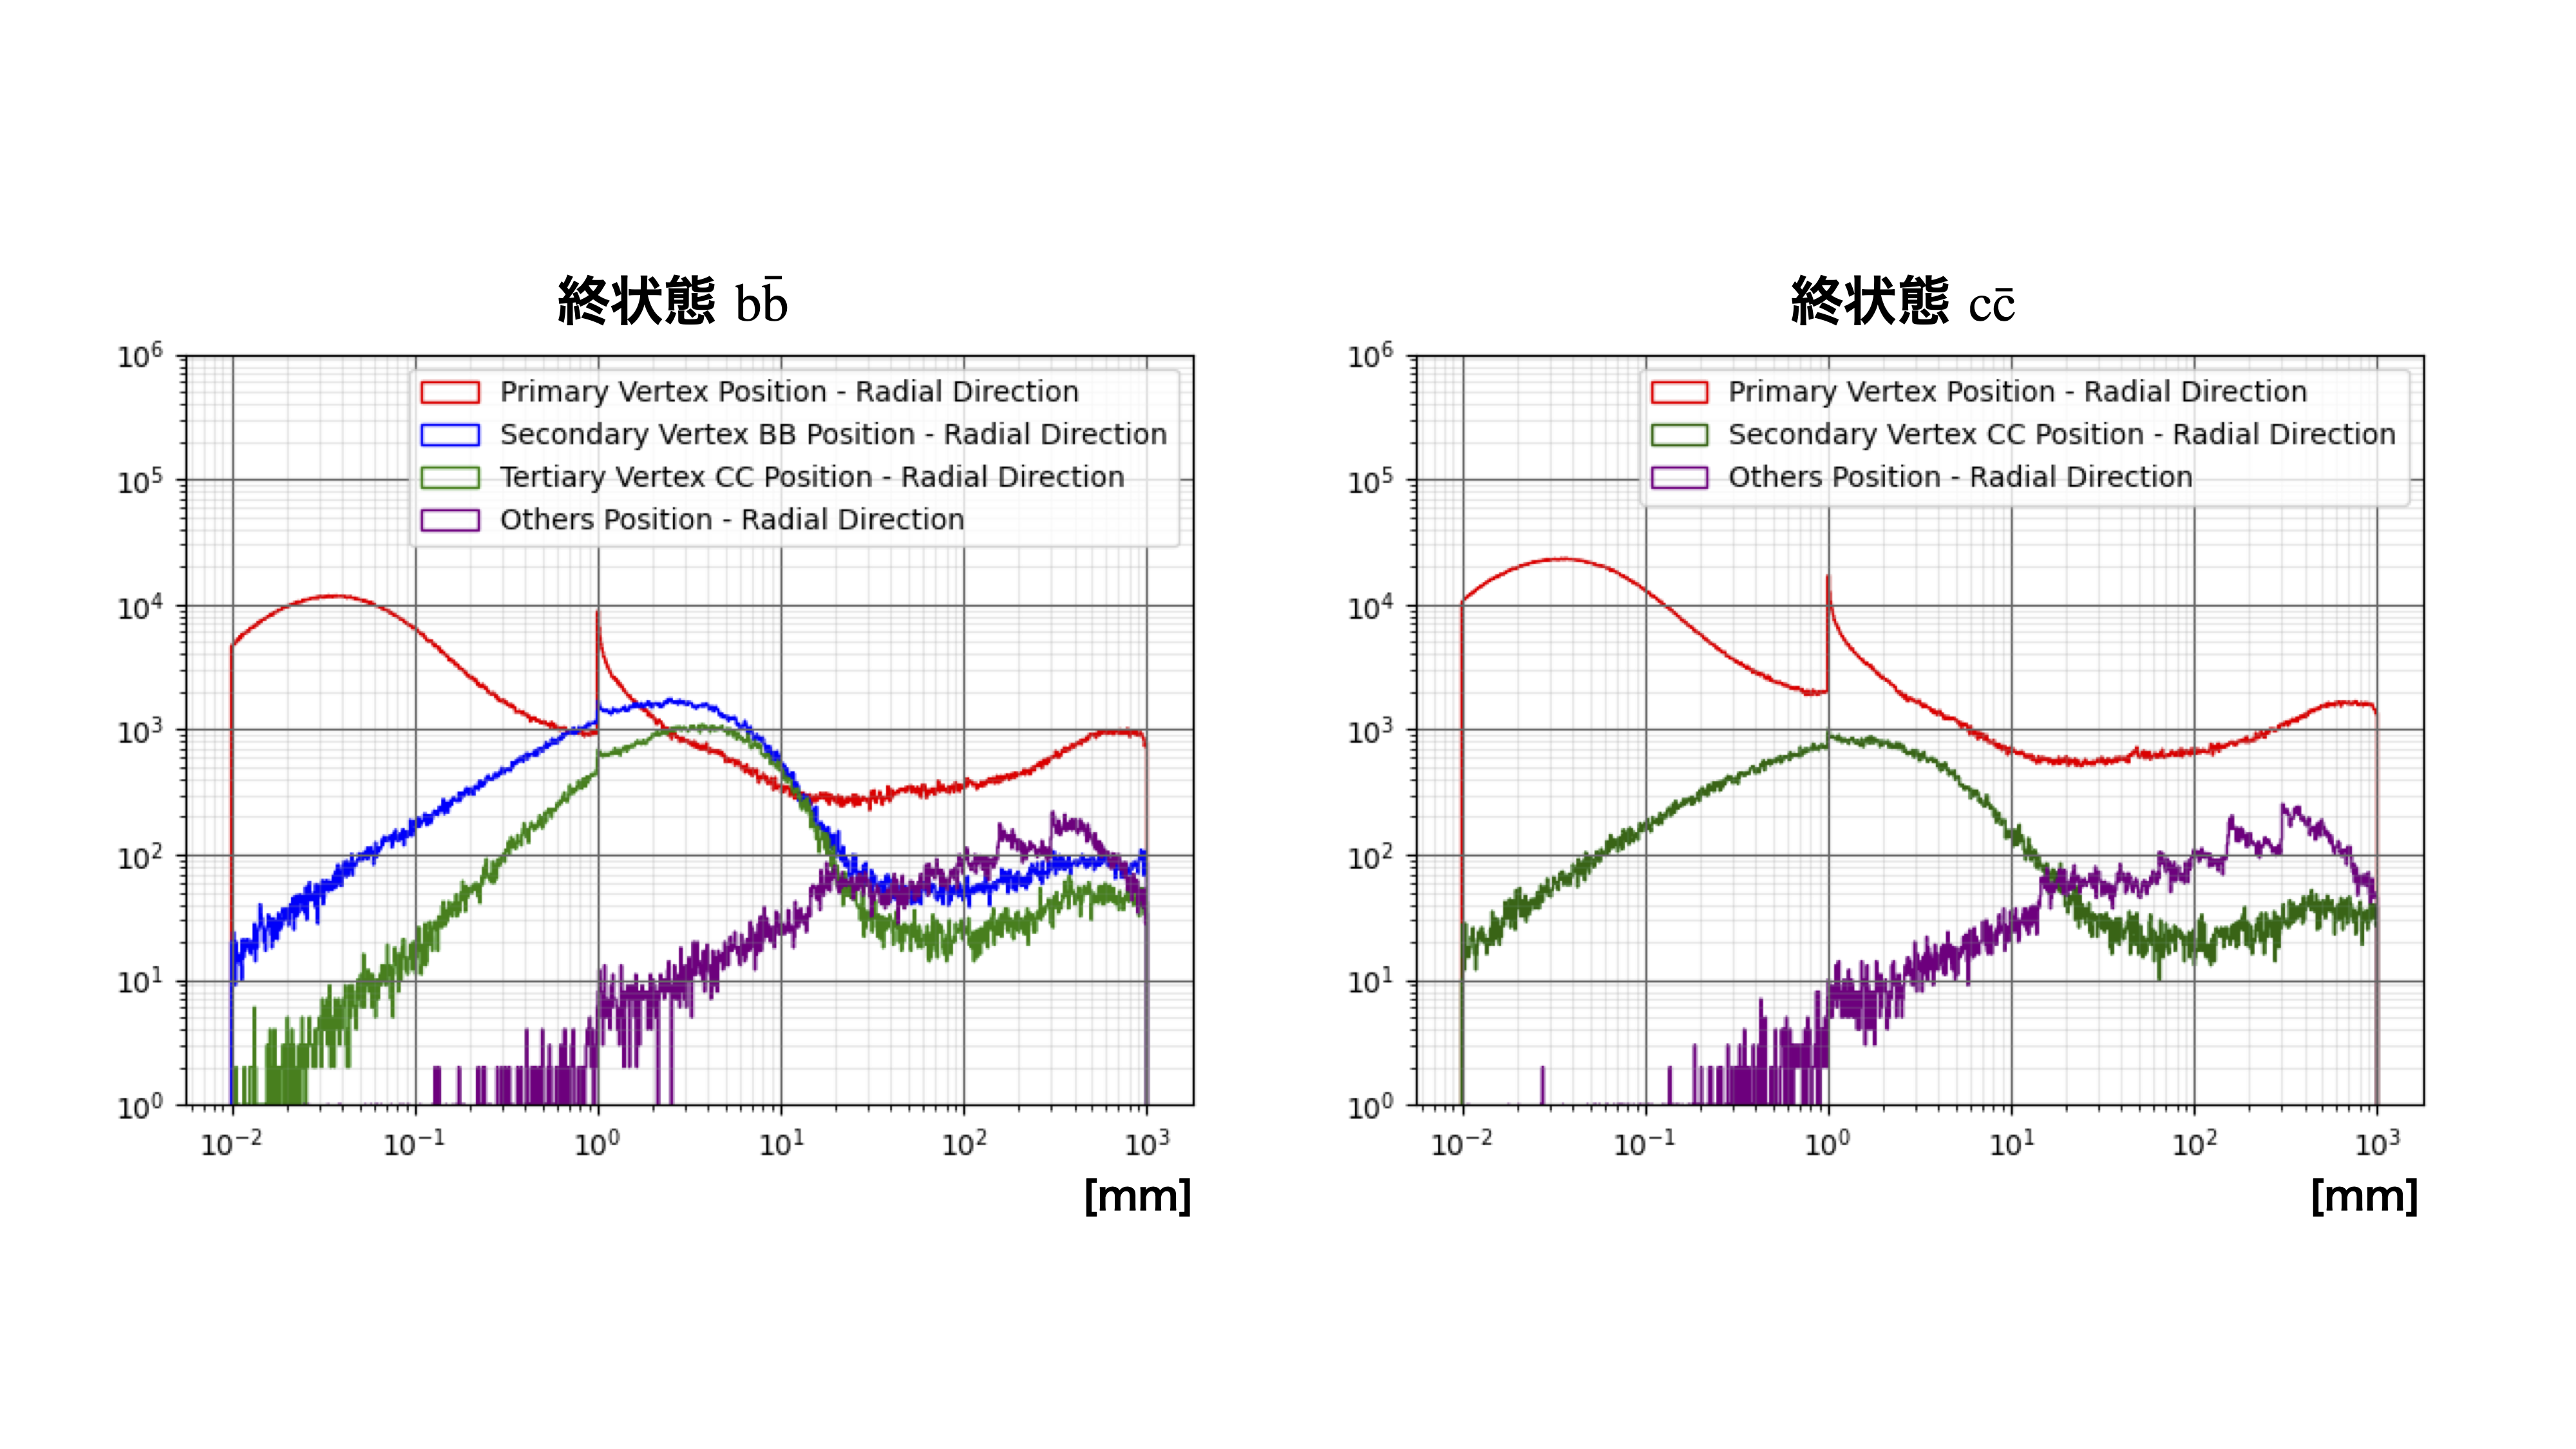
\includegraphics[trim = 50 100 50 150, width=1.0\textwidth, clip]{Figure/3Networks/3-1-2-3VertexPositions.png}
 \caption{LCFIPlusによって予想される崩壊点の位置の分布}
 \label{3-1-2-3VertexPositions}
\end{figure}

$1\ \mathrm{mm}$付近のピークはLCFIPlusのフィッティングが失敗している飛跡対である。
実際にフィッティング健全性を表す$\chi^2$との相関を見ると、図\ref{3-1-2-4VertexPositionsvsChiSquare}のように、$1\ \mathrm{mm}$付近のデータは大きな$\chi^2$値を持っていることが分かる。

\begin{figure}[htbp]
 \centering
 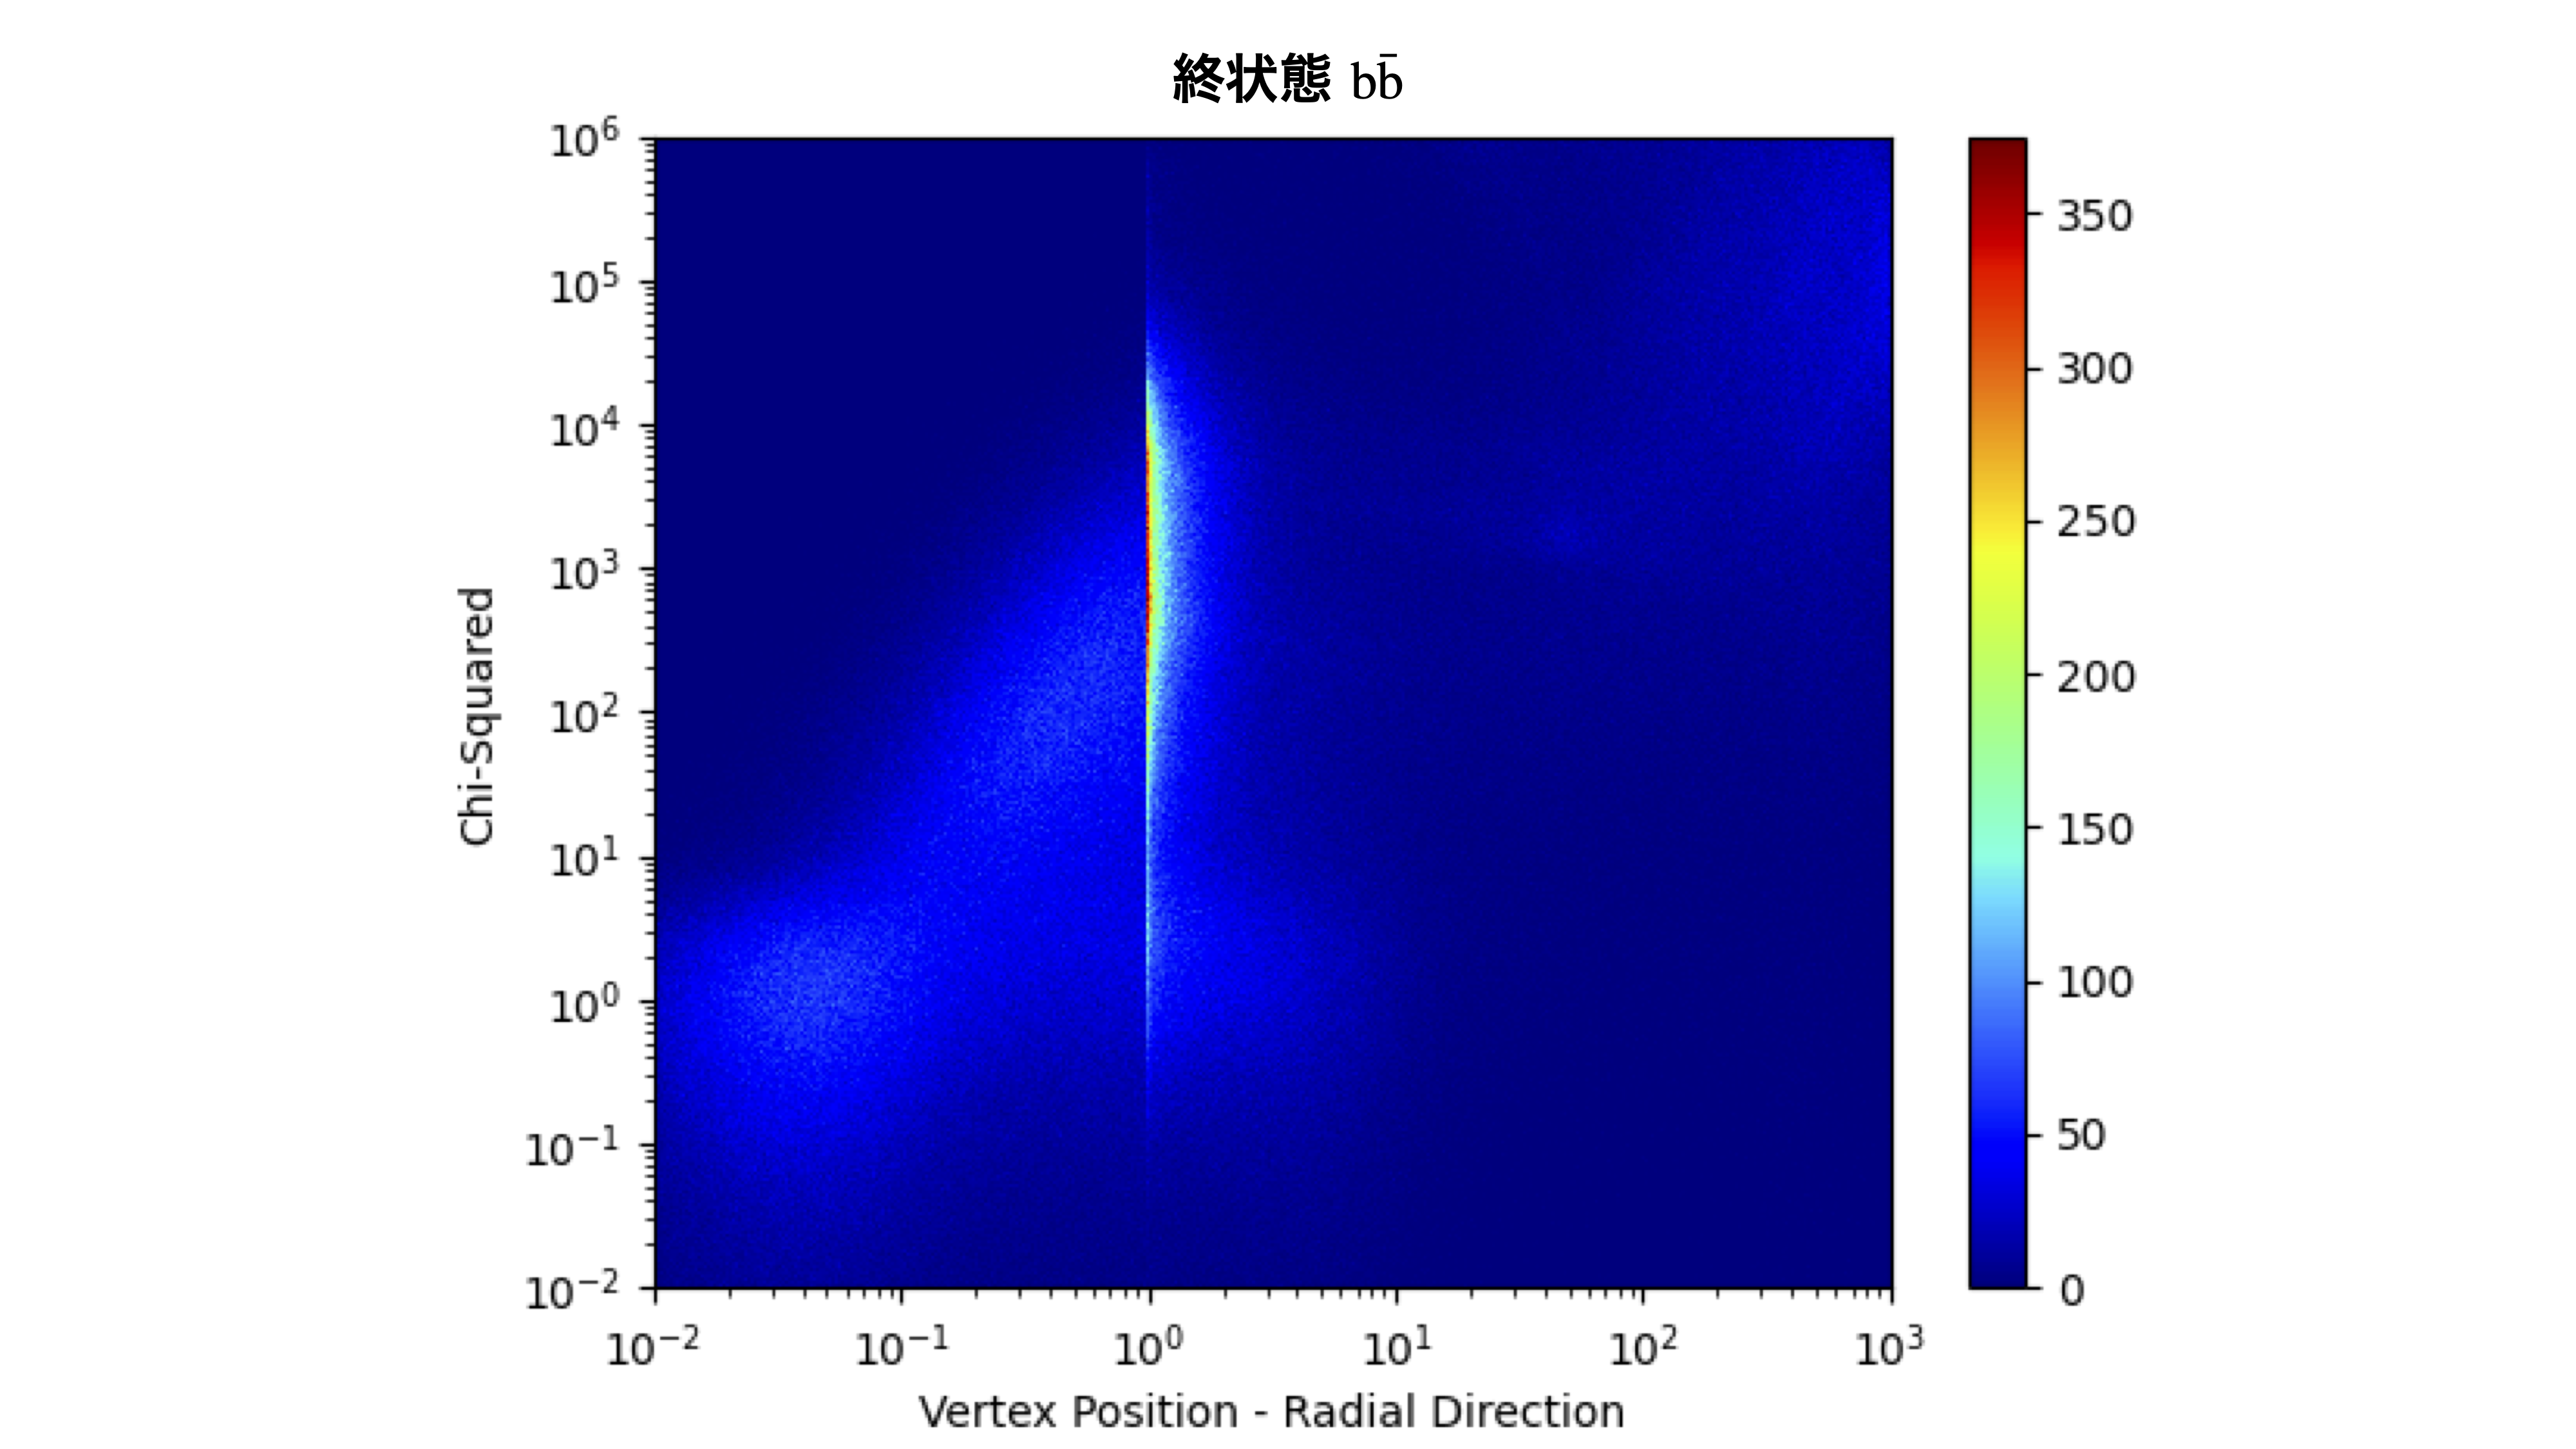
\includegraphics[width=1.0\textwidth, clip]{Figure/3Networks/3-1-2-4VertexPositionsvsChiSquare.png}
 \caption{LCFIPlusによって予想される崩壊点の位置と$\chi^2$の相関}
 \label{3-1-2-4VertexPositionsvsChiSquare}
\end{figure}

このように崩壊点の位置は崩壊点やフレーバーの分離に非常に重要な役割を果たしており、逆説的にある複数の飛跡について交点の位置 (崩壊点の位置) を再構成できなければ崩壊点種の分離は非常に難しくなる。


%%%%%%%%%%%%%%%%%%%%%%%%%%%%%%%%%%%%%%%%%%%%%%%%%%%%%%%%%%%%%%%%%%%%%%%%%%%%%%%%%%%%%%%%%%%%%%%%%%%%%
\section{深層学習を用いた崩壊点検出の実現} \label{Net:forVertexFinderwithDL}

深層学習は分類問題や回帰問題を解けるが、一方で基本的にはクラスタリングなど教師のいない学習には不向きである。
分類問題や回帰問題では訓練データからパターンを学び、データの持つ特徴量の空間内である種の境界を引く必要がある。
このパターンはあらゆるデータ内で分類可能な決まった性質を持っていなければならない。
例えば\ref{Net:Data:DataProperty}項では、同一フレーバーのSecondary Vertexが主に二つあることを解説した。
この二つのSecondary Vertexは事象内では位置の違いによって区別できるが、あらゆる事象間で不変的に一番や二番をラベル付けできる性質を持っていない。\footnote{実際には損失関数を最小にするような順序を与えることで分離することは可能であるが本研究においては現実的ではない。}
この同一フレーバーのSecondary Vertex間のラベルは人が決めた性質に過ぎず、本質的には順不同である。

崩壊点検出アルゴリズムの目的は崩壊点を探索することである。
したがって、同一フレーバーの複数のSecondary Vertexも識別せねばならない。
このような問題は一般にクラスタリングを用いて解くことが多いが、本研究で使用するデータは図\ref{3-1-1-2TracksandVertices}で示したように事象内に含まれる飛跡の本数や崩壊点の個数も異なっているという性質を持っている。
これはクラスター数やクラスターに含まれる要素数が常に変わってしまうということを意味しており、崩壊点検出をクラスタリングで行うことは不適であると判断した。

以上を踏まえた上で私は次の二つのネットワークを用いた崩壊点検出を提案する。

\begin{enumerate}
 \item 飛跡対についてのネットワーク
 \begin{itemize}
  \item 用途 : 崩壊点のタネの探索
  \item 入力 : 事象内のあらゆる飛跡対 (全ての二本の飛跡の組み合わせ)
  \item 出力 : 飛跡対が結合しているか否か・崩壊点の位置
 \end{itemize}
 \item 任意の数の飛跡についてのネットワーク
 \begin{itemize}
  \item 用途 : 崩壊点の生成
  \item 入力 : 崩壊点のタネ・事象内の全ての飛跡
  \item 出力 : 事象内のそれぞれの飛跡が崩壊点のタネに結合しているか否か
 \end{itemize}
\end{enumerate}

飛跡対のついてのネットワークは崩壊点のタネとなる飛跡対を探索するだけであるので、単体では崩壊点を形成することはできない。
そこで、私は崩壊点の生成を行う、もう一つのネットワークを構築した。
任意の数の飛跡についてのネットワークは崩壊点のタネを初期状態として、そこに飛跡を一本ずつ加え崩壊点の生成を行うネットワークである。
本研究は以上の二つのネットワークを用いることで崩壊点検出を実現した。
構造や学習についてのより詳細な個々のネットワークの解説は、後の\ref{Net:PairModel}節や\ref{Net:VertexLSTM}節で述べる。

Tensorflow/Kerasフレームワークを用いてこれらのネットワークの構築・学習を行なった。
また、学習に際しては計算機として、弊研究室サーバーの"NVIDIA TITAN RTX"や九州大学情報基盤研究開発センター研究用計算機システムの一般利用を使用した。
以下詳細なソフトウェア・ハードウェアの環境を表\ref{SoftwareHardwareEnvironments}に示す。

\begin{table}[htb]
 \centering
 \small
  \begin{tabular}{l c} \hline
    ソフトウェア&\\\hline\hline
    Python & $3.6.8$\\
    Tensorflow & $2.1.0$\\
    Keras & $2.3.1$\\\hline
    ハードウェア &\\\hline\hline
    CPU& AMD EPYC 7402P 24-Core Processor 48個\\
    メモリ & $263694036\ \mathrm{kB}$\\
    GPU & NVIDIA Corporation TU102 [TITAN RTX] 2個\\\hline
  \end{tabular}
  \caption{ソフトウェア・ハードウェアの環境}
  \label{SoftwareHardwareEnvironments}
\end{table}


%%%%%%%%%%%%%%%%%%%%%%%%%%%%%%%%%%%%%%%%%%%%%%%%%%%%%%%%%%%%%%%%%%%%%%%%%%%%%%%%%%%%%%%%%%%%%%%%%%%%%
\section{飛跡対についてのネットワーク} \label{Net:PairModel}

ここでは\ref{Net:forVertexFinderwithDL}節で紹介した二つのネットワークの内、飛跡対についてのネットワークに関して述べる。
主にネットワークの構造に関しては\ref{Net:PM:StructureofPM}項で、学習に関しては\ref{Net:PM:TrainingandStrategyofPM}項で解説する。
また、そのようにして構築、訓練されたネットワーク単体についての性能と評価に関しては、\ref{Net:PM:PerformanceofPM}項で述べることとする。

飛跡対についてのネットワークは、崩壊点のタネを探索するためのネットワークであり、入力は二本の飛跡についての情報、出力は飛跡対についての崩壊点の種類や位置である。
この崩壊点の種類を考える上で\ref{Net:Data:DataProperty}項で述べた終状態による崩壊点種の差異を考えなければならない。
例えば、終状態が$\rm b\bar{b}$の場合は$\rm b \to c$という崩壊過程を辿り、ボトム・フレーバーのSecondary Vertexとチャーム・フレーバーのTertiary Vertexが生じ、終状態が$\rm c\bar{c}$の場合はチャーム・フレーバーのSecondary Vertexが生じる。
また両方の終状態について、これら以外の崩壊点であるOthers\footnote{タウ粒子の崩壊やストレンジ ($\rm s$) ・フレーバーのハドロンの崩壊、光子変換}を考える必要がある。
更に終状態$\rm b\bar{b}$の場合について、ボトム・フレーバーのSecondary Vertexからの飛跡とそこから生じたチャーム・フレーバーのTertiary Vertexからの飛跡を一本ずつ含んだ飛跡対を準崩壊点として定義する。 (図\ref{3-3-0-1SecondaryVertexBC}) 

以上より、飛跡対についての崩壊点種は"非結合な飛跡対 (Not Connected, NC)"、"Primary Vertex (PV)"、"チャーム・フレーバーのSecondary Vertex (SVCC)"、"ボトム・フレーバーのSecondary Vertex (SVBB)"、"チャーム・フレーバーのTertiary Vertex (TVCC)"、"終状態$\rm b\bar{b}$での準崩壊点 (SVBC)"、"これら以外の崩壊点 (Others)"の計$7$つとなる。

\begin{figure}[htbp]
 \centering
 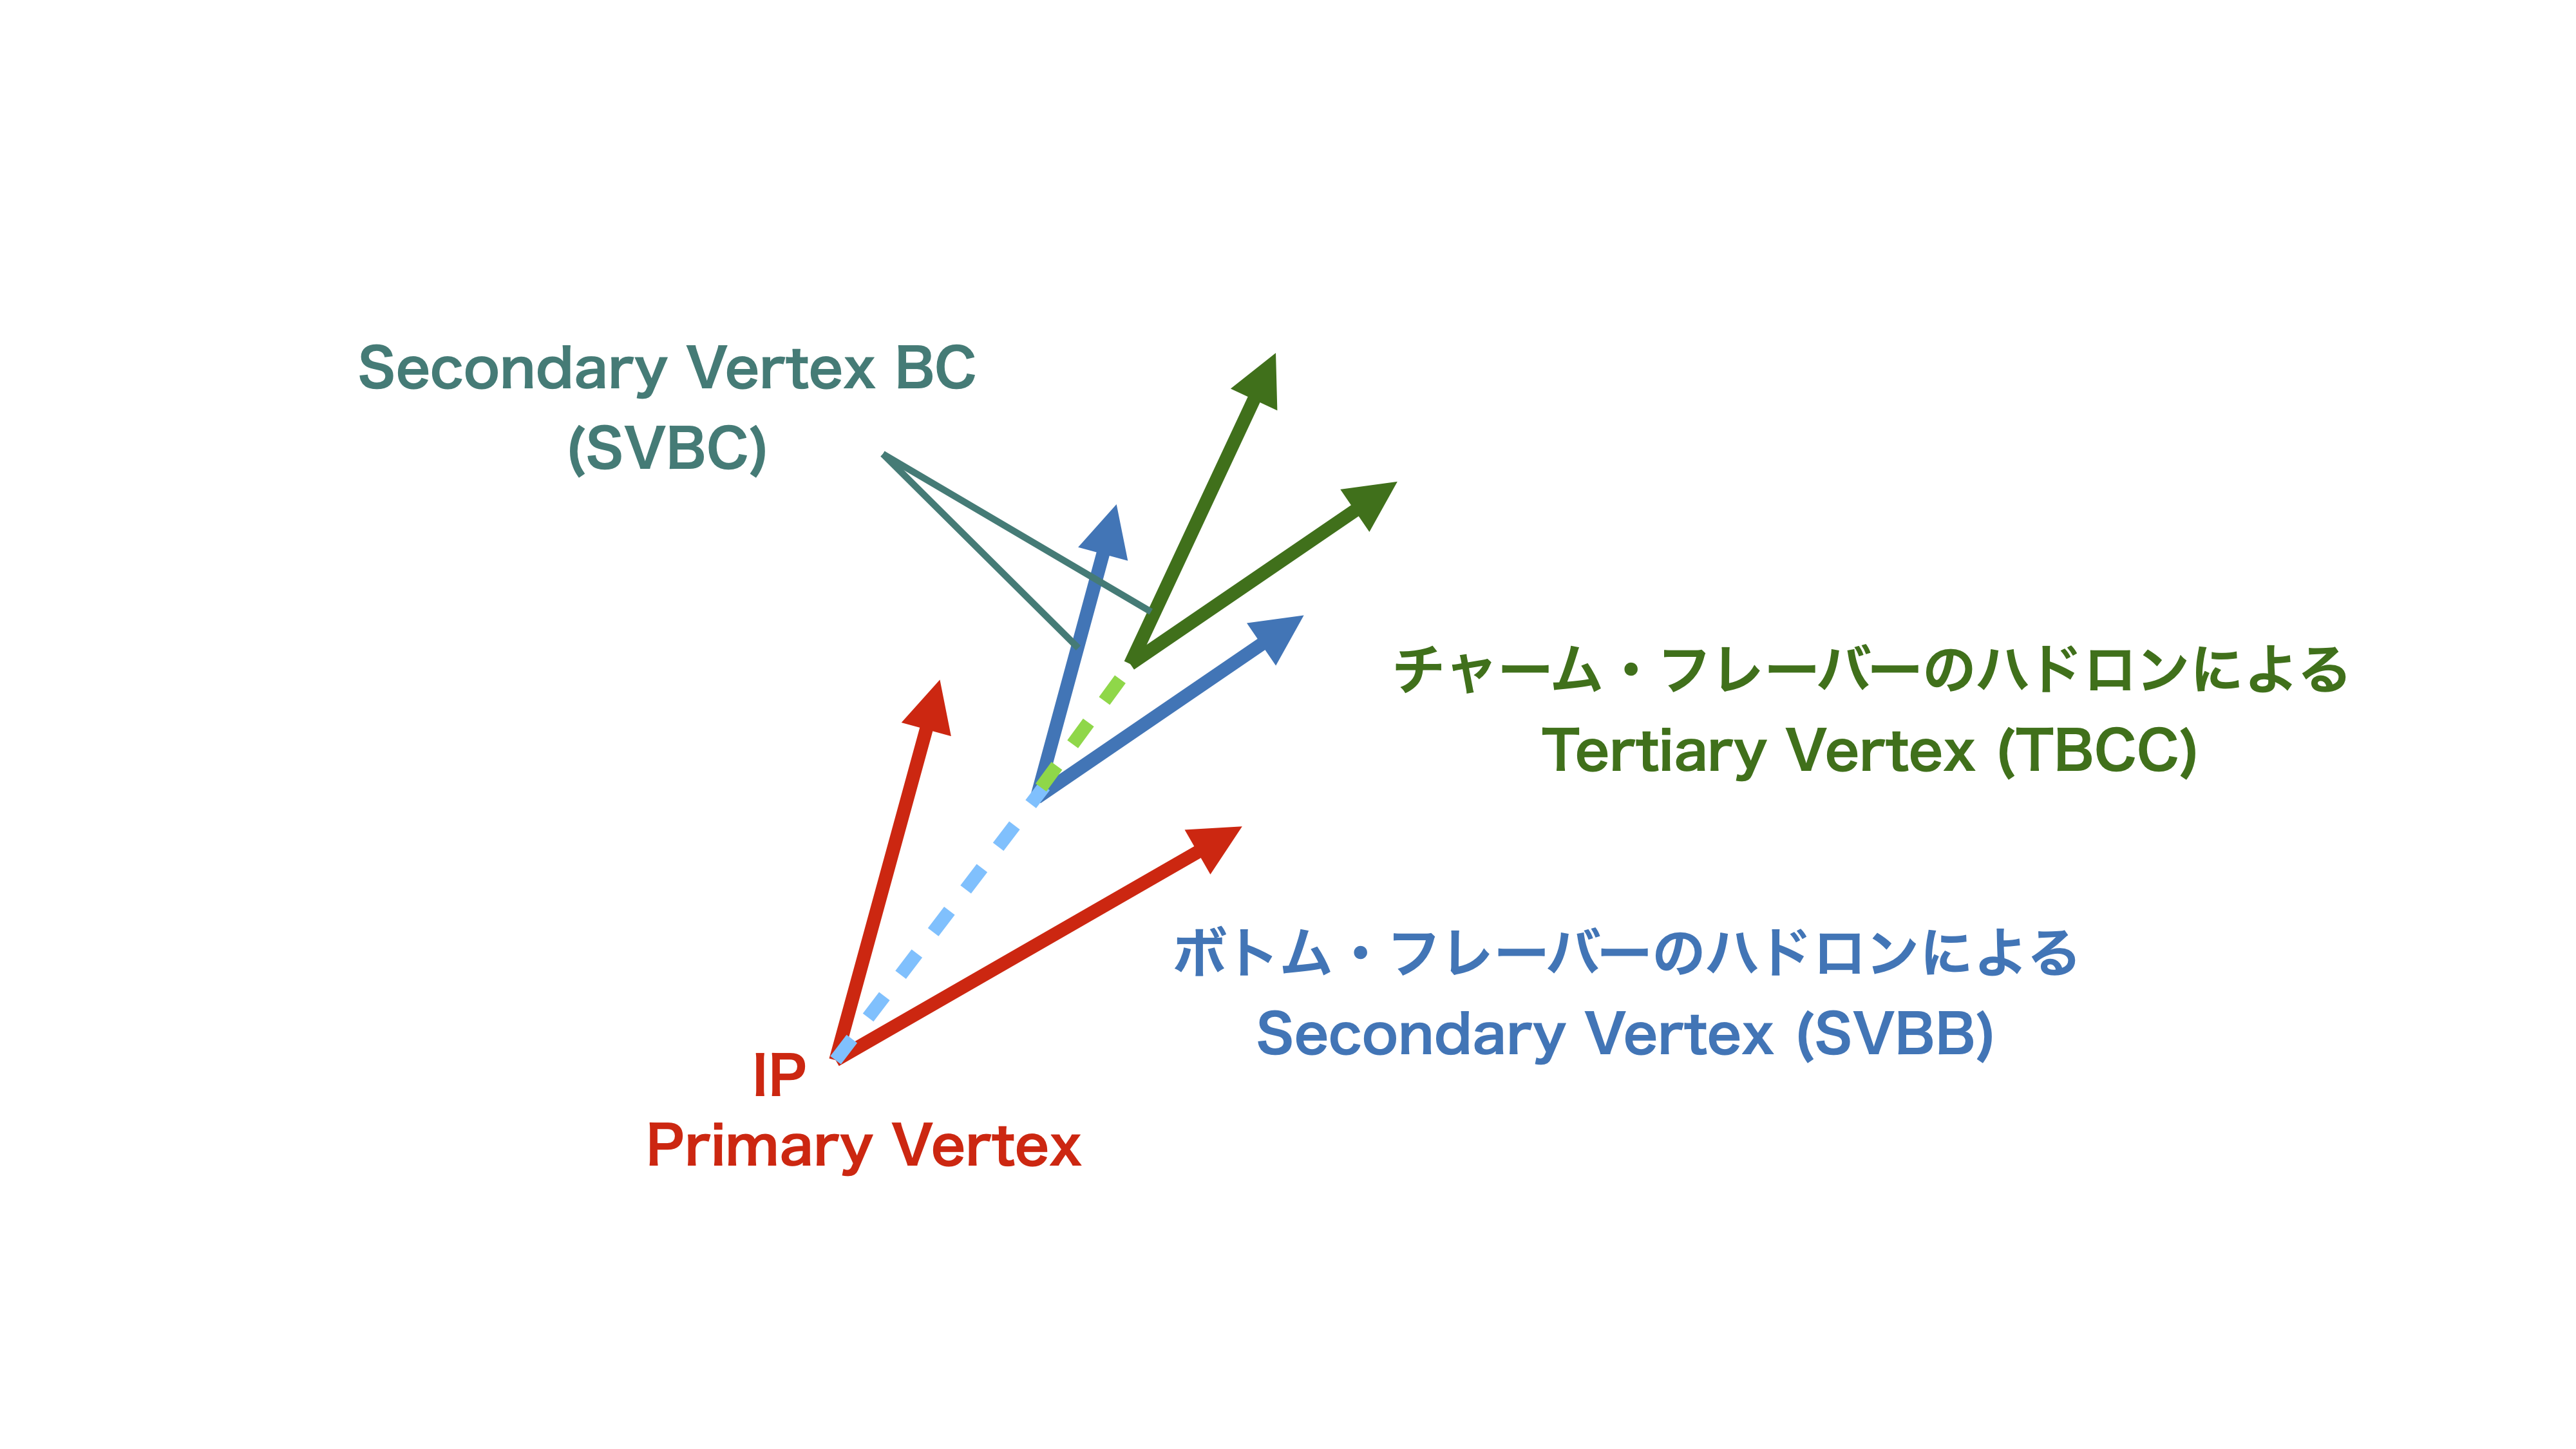
\includegraphics[trim = 200 150 200 150, width=0.9\textwidth, clip]{Figure/3Networks/3-3-0-1SecondaryVertexBC.png}
 \caption{終状態$\rm b\bar{b}$での崩壊点}
 \label{3-3-0-1SecondaryVertexBC}
\end{figure}

崩壊点の位置についての訓練データを作成するに当たって、正解ラベルとして図\ref{3-1-2-3VertexPositions}のLCFIPlusのフィッティングで得られる予測値を用いた。
こちらは回帰によって値を再現し、崩壊点のタネの選別に補助として活用する。


%%%%%%%%%%%%%%%%%%%%%%%%%%%%%%%%%%%%%%%%%%%%%%%%%%%%%%%%%%%%%%%%%%%%%%%%
\subsection{ネットワークの構造} \label{Net:PM:StructureofPM}

飛跡対についてのネットワークとして非常にシンプルなフィードフォーワード構造を使用した。
ネットワークの概略図を図\ref{3-3-1-1PairModel}に示す。

\begin{figure}[htbp]
 \centering
 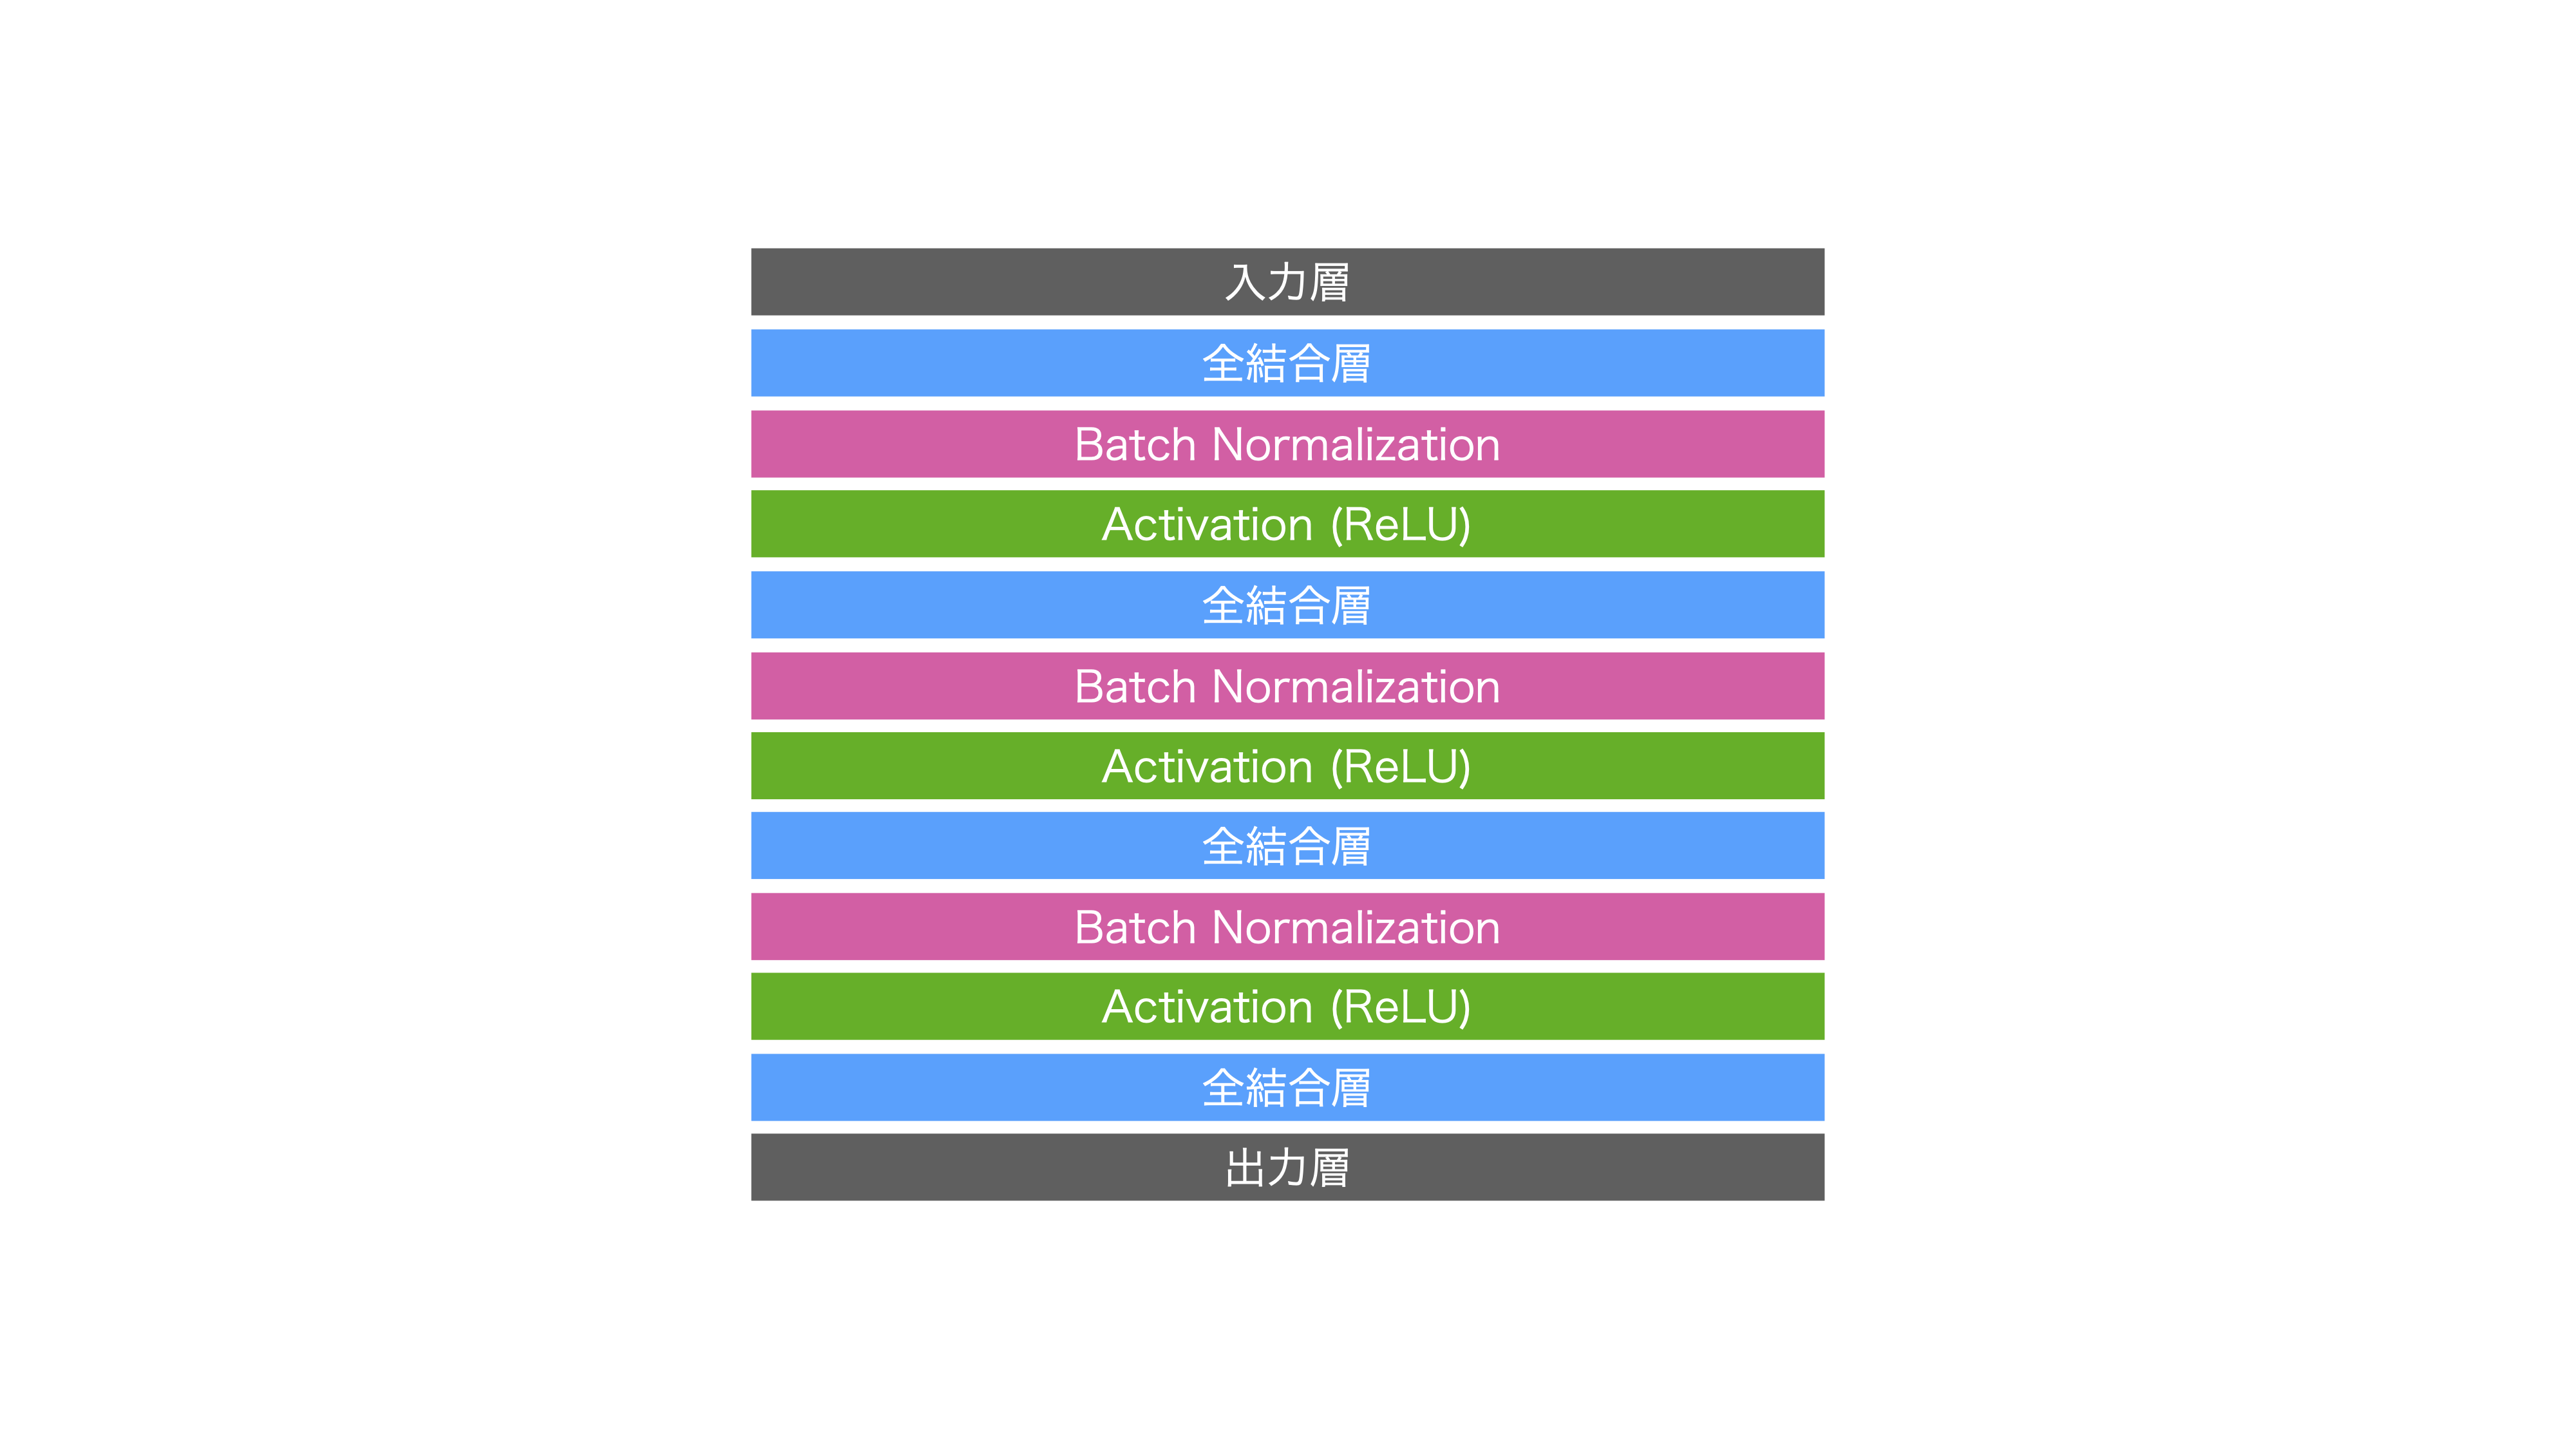
\includegraphics[trim = 200 50 200 50, width=0.9\textwidth, clip]{Figure/3Networks/3-3-1-1PairModel.png}
 \caption{飛跡対についてのネットワークの概略図}
 \label{3-3-1-1PairModel}
\end{figure}

前述したように出力は、7クラス分類と回帰1つである。
出力の直前の全結合層で分類問題と回帰問題に分離している。
また、過学習 (Over fitting) を避ける為、Batch Normalization\cite{BatchNormalizationpaper}を全結合層の後に配置している。
過学習とは、ネットワークが過度に訓練データに適合してしまい、検証データやテストデータへの汎化性能が悪化してしまう教師あり学習の問題の一つである。
また勾配消失への対策として、活性化関数は全てReLU関数を使用している。


%%%%%%%%%%%%%%%%%%%%%%%%%%%%%%%%%%%%%%%%%%%%%%%%%%%%%%%%%%%%%%%%%%%%%%%%
\subsection{ネットワークの学習と戦略} \label{Net:PM:TrainingandStrategyofPM}

訓練データは事象中の全ての飛跡対の組み合わせを考える。
よって入力変数は飛跡についての情報である$22$個の変数が飛跡二本分であるので合計$44$個である。
ここで次の二つの事柄に注意せねばならない。

\begin{itemize}
 \item 分類クラスは二つの終状態$\rm b\bar{b}$と$\rm c\bar{c}$を合わせたものである
 \item 分類クラスのデータ数の比がNCやPVが支配的な不均衡データ (Imbalanced Data) となる
\end{itemize}

各終状態での分類クラスのデータ数の比を図\ref{3-3-2-1ImbalancedData}に示す。

\begin{figure}[htbp]
 \centering
 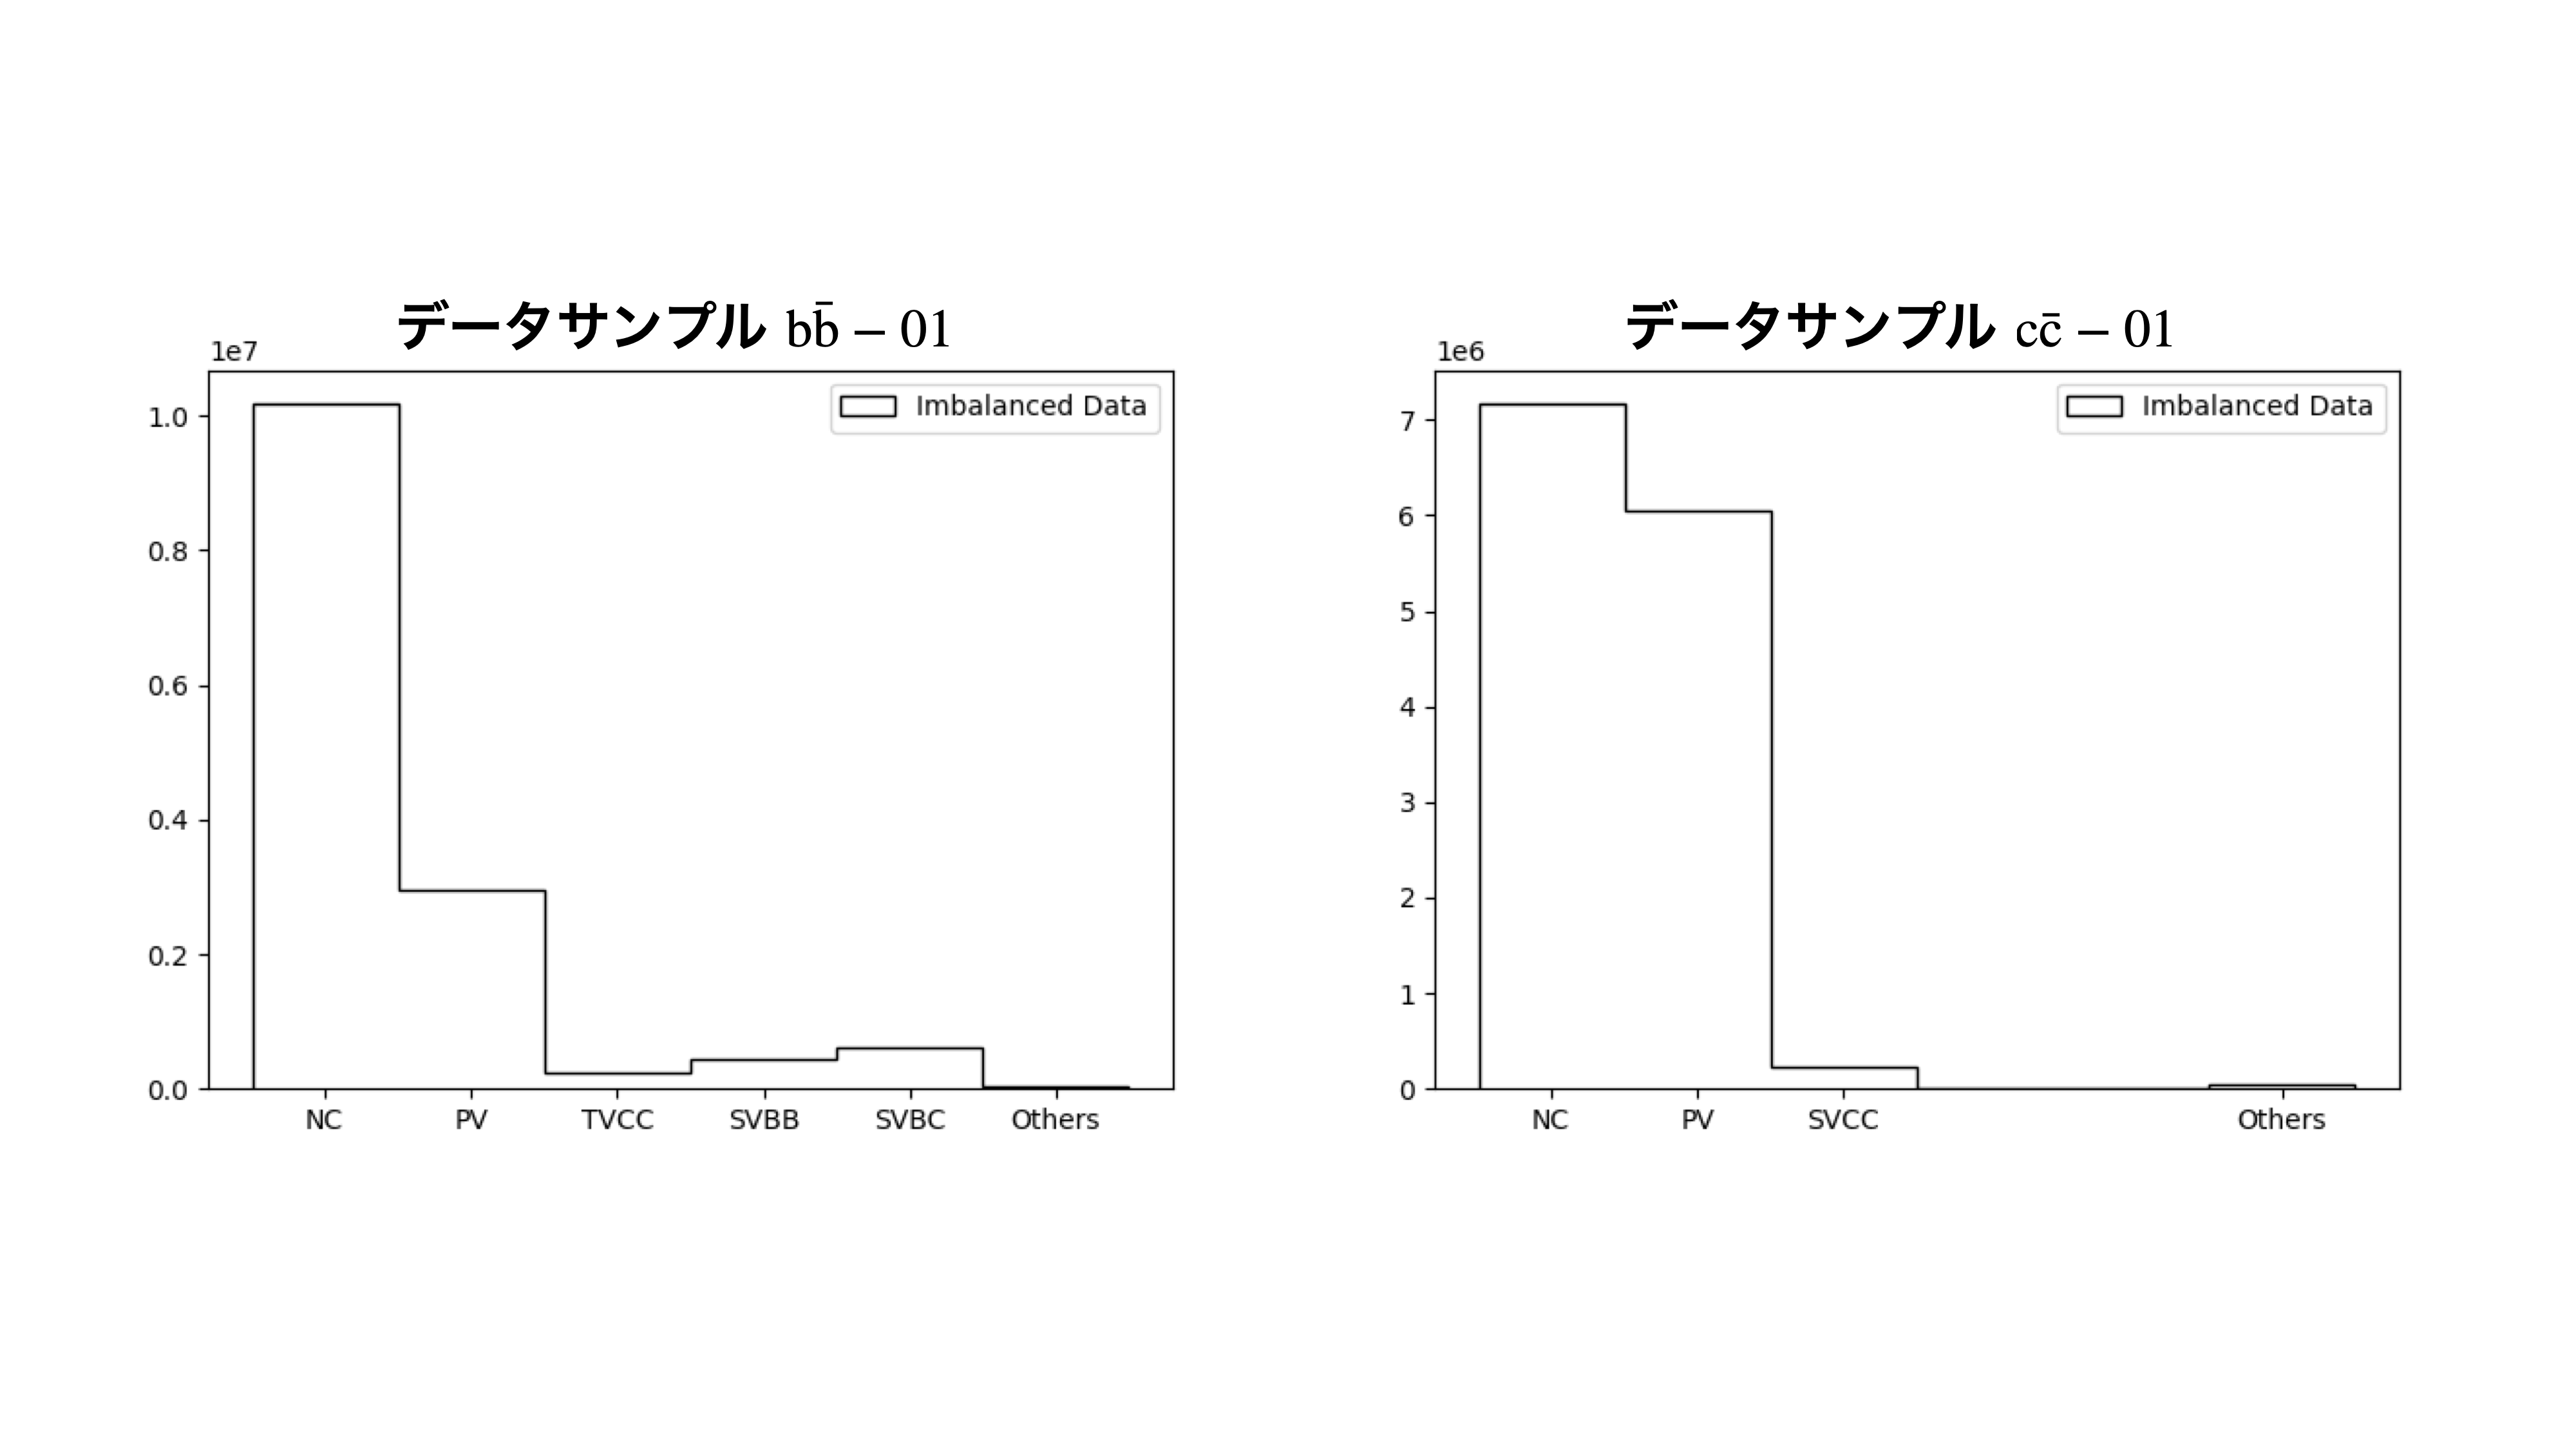
\includegraphics[trim = 100 200 100 150, width=0.9\textwidth, clip]{Figure/3Networks/3-3-2-1ImbalancedData.png}
 \caption{各終状態での分類クラスのデータ数の比}
 \label{3-3-2-1ImbalancedData}
\end{figure}

このような不均衡データについては、少数クラスのデータをかさ増しするオーバーサンプリング、多数クラスのデータを間引くアンダーサンプリング、損失関数のコストに重みをつけるコスト考慮型学習の主に三つの対応策が存在する。
オーバーサンプリングやアンダーサンプリングは過学習や情報の欠損などの問題を抱えているため、本研究では基本的にコスト考慮型学習を用いる。
ただし、二つの終状態のデータを単純に足し合わせた場合、共通する分類クラスであるNCやPVがより顕著になり、他クラスの分類が不十分になると考えられる。
このためNCやPVに関しては各終状態毎に半分にランダムサンプリングし足し合わせた。
最終的な訓練データでの分類クラスのデータ数の比を図\ref{3-3-2-2ImbalancedData}に示す。

\begin{figure}[htbp]
 \centering
 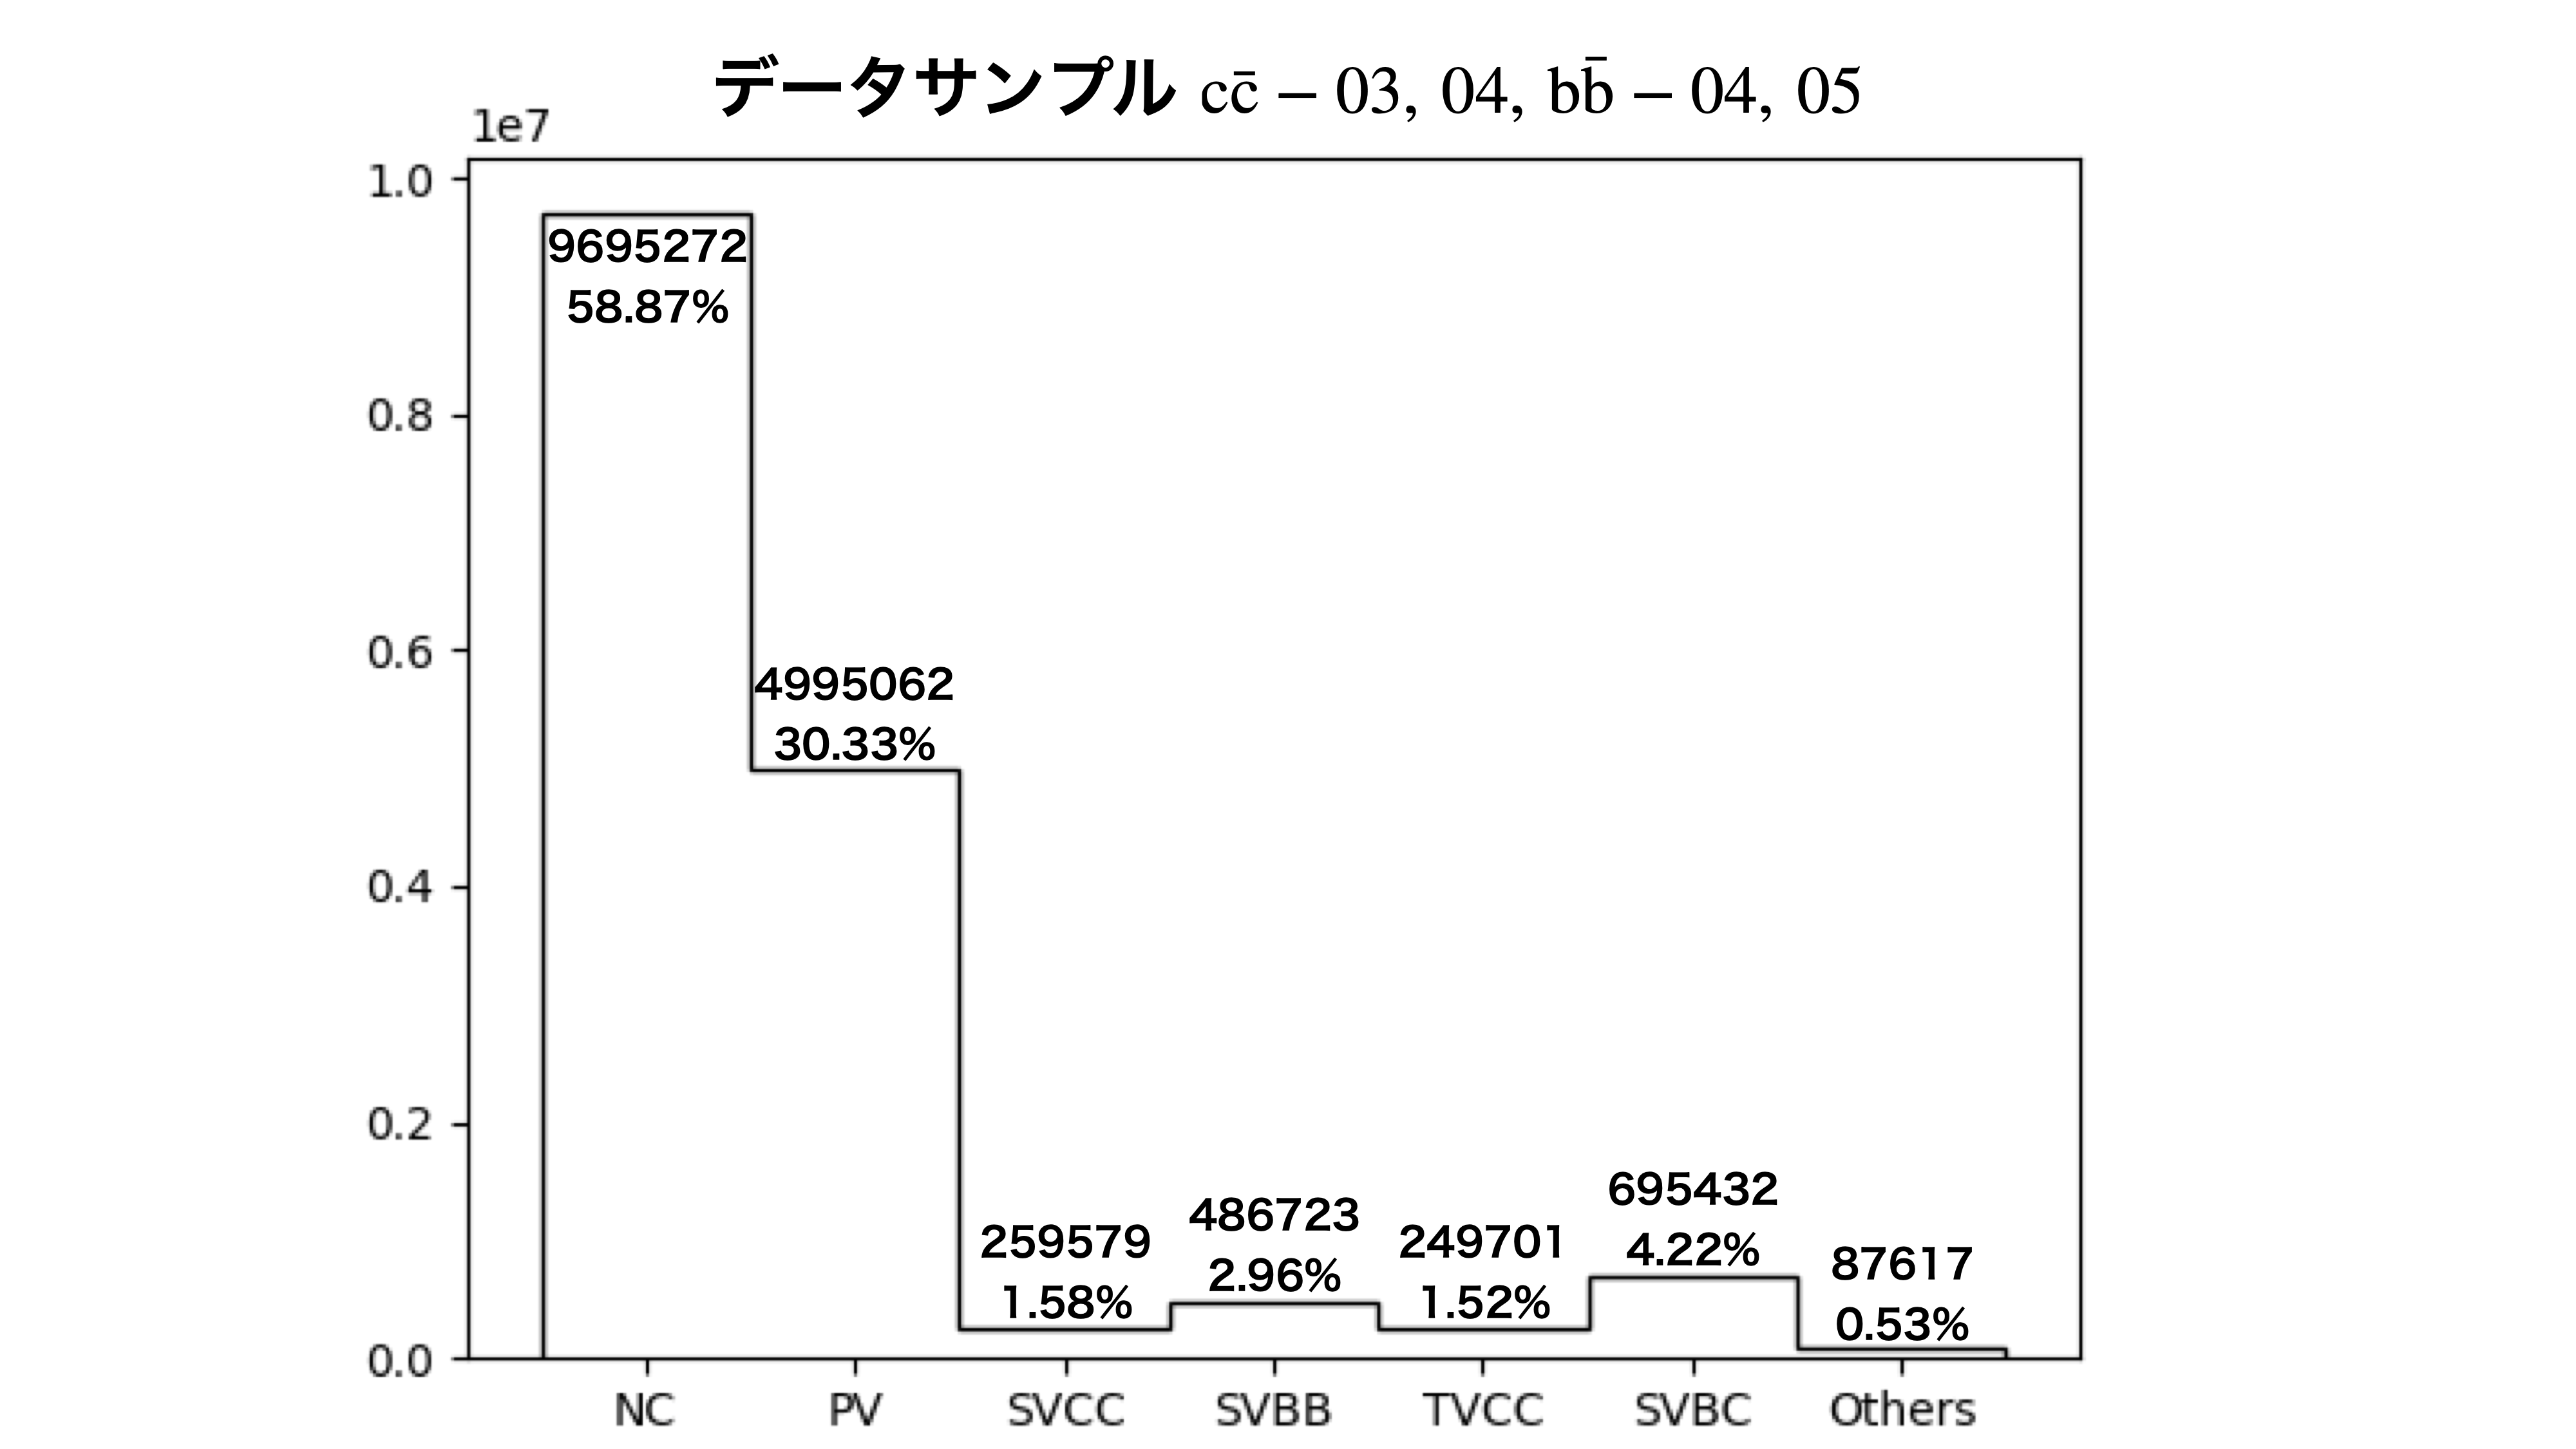
\includegraphics[width=1.0\textwidth]{Figure/3Networks/3-3-2-2ImbalancedData.png}
 \caption{訓練データでの分類クラスのデータ数の比}
 \label{3-3-2-2ImbalancedData}
\end{figure}

損失関数$L$は分類問題である崩壊点の種類に関しての損失関数$L_{\rm CE}$と回帰問題である崩壊点の位置に関しての損失関数$L_{\rm LMSE}$の二つの合計となる。
本研究では、損失関数$L_{\rm CE}$の各クラスへの重みは分類クラスの数の比の逆数を使用し不均衡データへ対策を行なった。
ここでは最も数の少ないOthersの重みを$1$としている。
\begin{equation}
 \begin{split}
 L_{\rm CE} = & - 0.0090\  t_{\rm NC} \log{(y_{\rm NC})} - 0.0175\  t_{\rm PV} \log{(y_{\rm PV})} \\
       & - 0.3375\  t_{\rm SVCC} \log{(y_{\rm SVCC})} - 0.1800\  t_{\rm SVBB} \log{(y_{\rm SVBB})}\\
       & - 0.3509\  t_{\rm TVCC} \log{(y_{\rm TVCC})} - 0.1260\  t_{\rm SVBC} \log{(y_{\rm SVBC})}\\
       & - 1.0\  t_{\rm Others} \log{(y_{\rm Others})}\\
 \end{split}
\end{equation}
崩壊点の位置についての損失関数$L_{\rm LMSE}$として平均二乗誤差を使用した。
ただし、図\ref{3-1-2-3VertexPositions}からも分かるようにその値は非常に広い範囲に分布しているため、出力や正解ラベルの対数を使用し
\begin{equation}
 \begin{split}
 L_{\rm LMSE} = (\log{(t_{\rm Position})} - \log{(y_{\rm Position})})^2
 \end{split}
\end{equation}
とした。

したがって、飛跡対についてのネットワークの損失関数$L$は
\begin{equation}
 \begin{split}
 L & = w_{\rm vertex} L_{\rm CE} + w_{\rm position} L_{\rm LMSE}
 \end{split}
\end{equation}
となる。
ここで、$w_{\rm vertex},\ w_{\rm position}$は各損失関数$L_{\rm CE},\ L_{\rm LMSE}$への重みである。
今回は崩壊点の位置を学習した後に崩壊点種の分類を行なった。
これは崩壊点の位置、あるいはそのような情報を抽出できるネットワークのパラメータを利用して、崩壊点種の分類を行なって欲しいという狙いからである。
このような手法は転移学習 (Transfer Learning, TL) やファインチューニングという手法\footnote{これらの手法ではあらかじめ学習済みのネットワークを別の問題解決に活用するテクニックである}に似た発想であるが、今回はこれら二つの手法とは異なり、ネットワークの重みは全て再学習に使用している。
学習は以下の手順で行う。

\begin{enumerate}
 \item $(w_{\rm vertex},\ w_{\rm position})=(0.1,\ 0.9)$、$1000\ \mathrm{epoch}$、学習率${\rm LR}=0.001$
 \item $(w_{\rm vertex},\ w_{\rm position})=(0.9,\ 0.1)$、$1500\ \mathrm{epoch}$、学習率${\rm LR}=0.001$
 \item $(w_{\rm vertex},\ w_{\rm position})=(0.8,\ 0.2)$、$500\ \mathrm{epoch}$、学習率${\rm LR}=0.0001$
\end{enumerate}

また、重み更新の最適化手法としてSGDを用いた。
これは、Adamなどでは収束が早すぎ、過学習になる恐れがあったためである。
学習には$13175508$サンプル、検証には$3293878$サンプルのデータを使用した。
エポック数を横軸に、正答率と損失を縦軸にプロットした学習曲線を図\ref{3-3-2-2TrainingCurve}に示す。

%\begin{figure}[htbp]
 %\centering
 %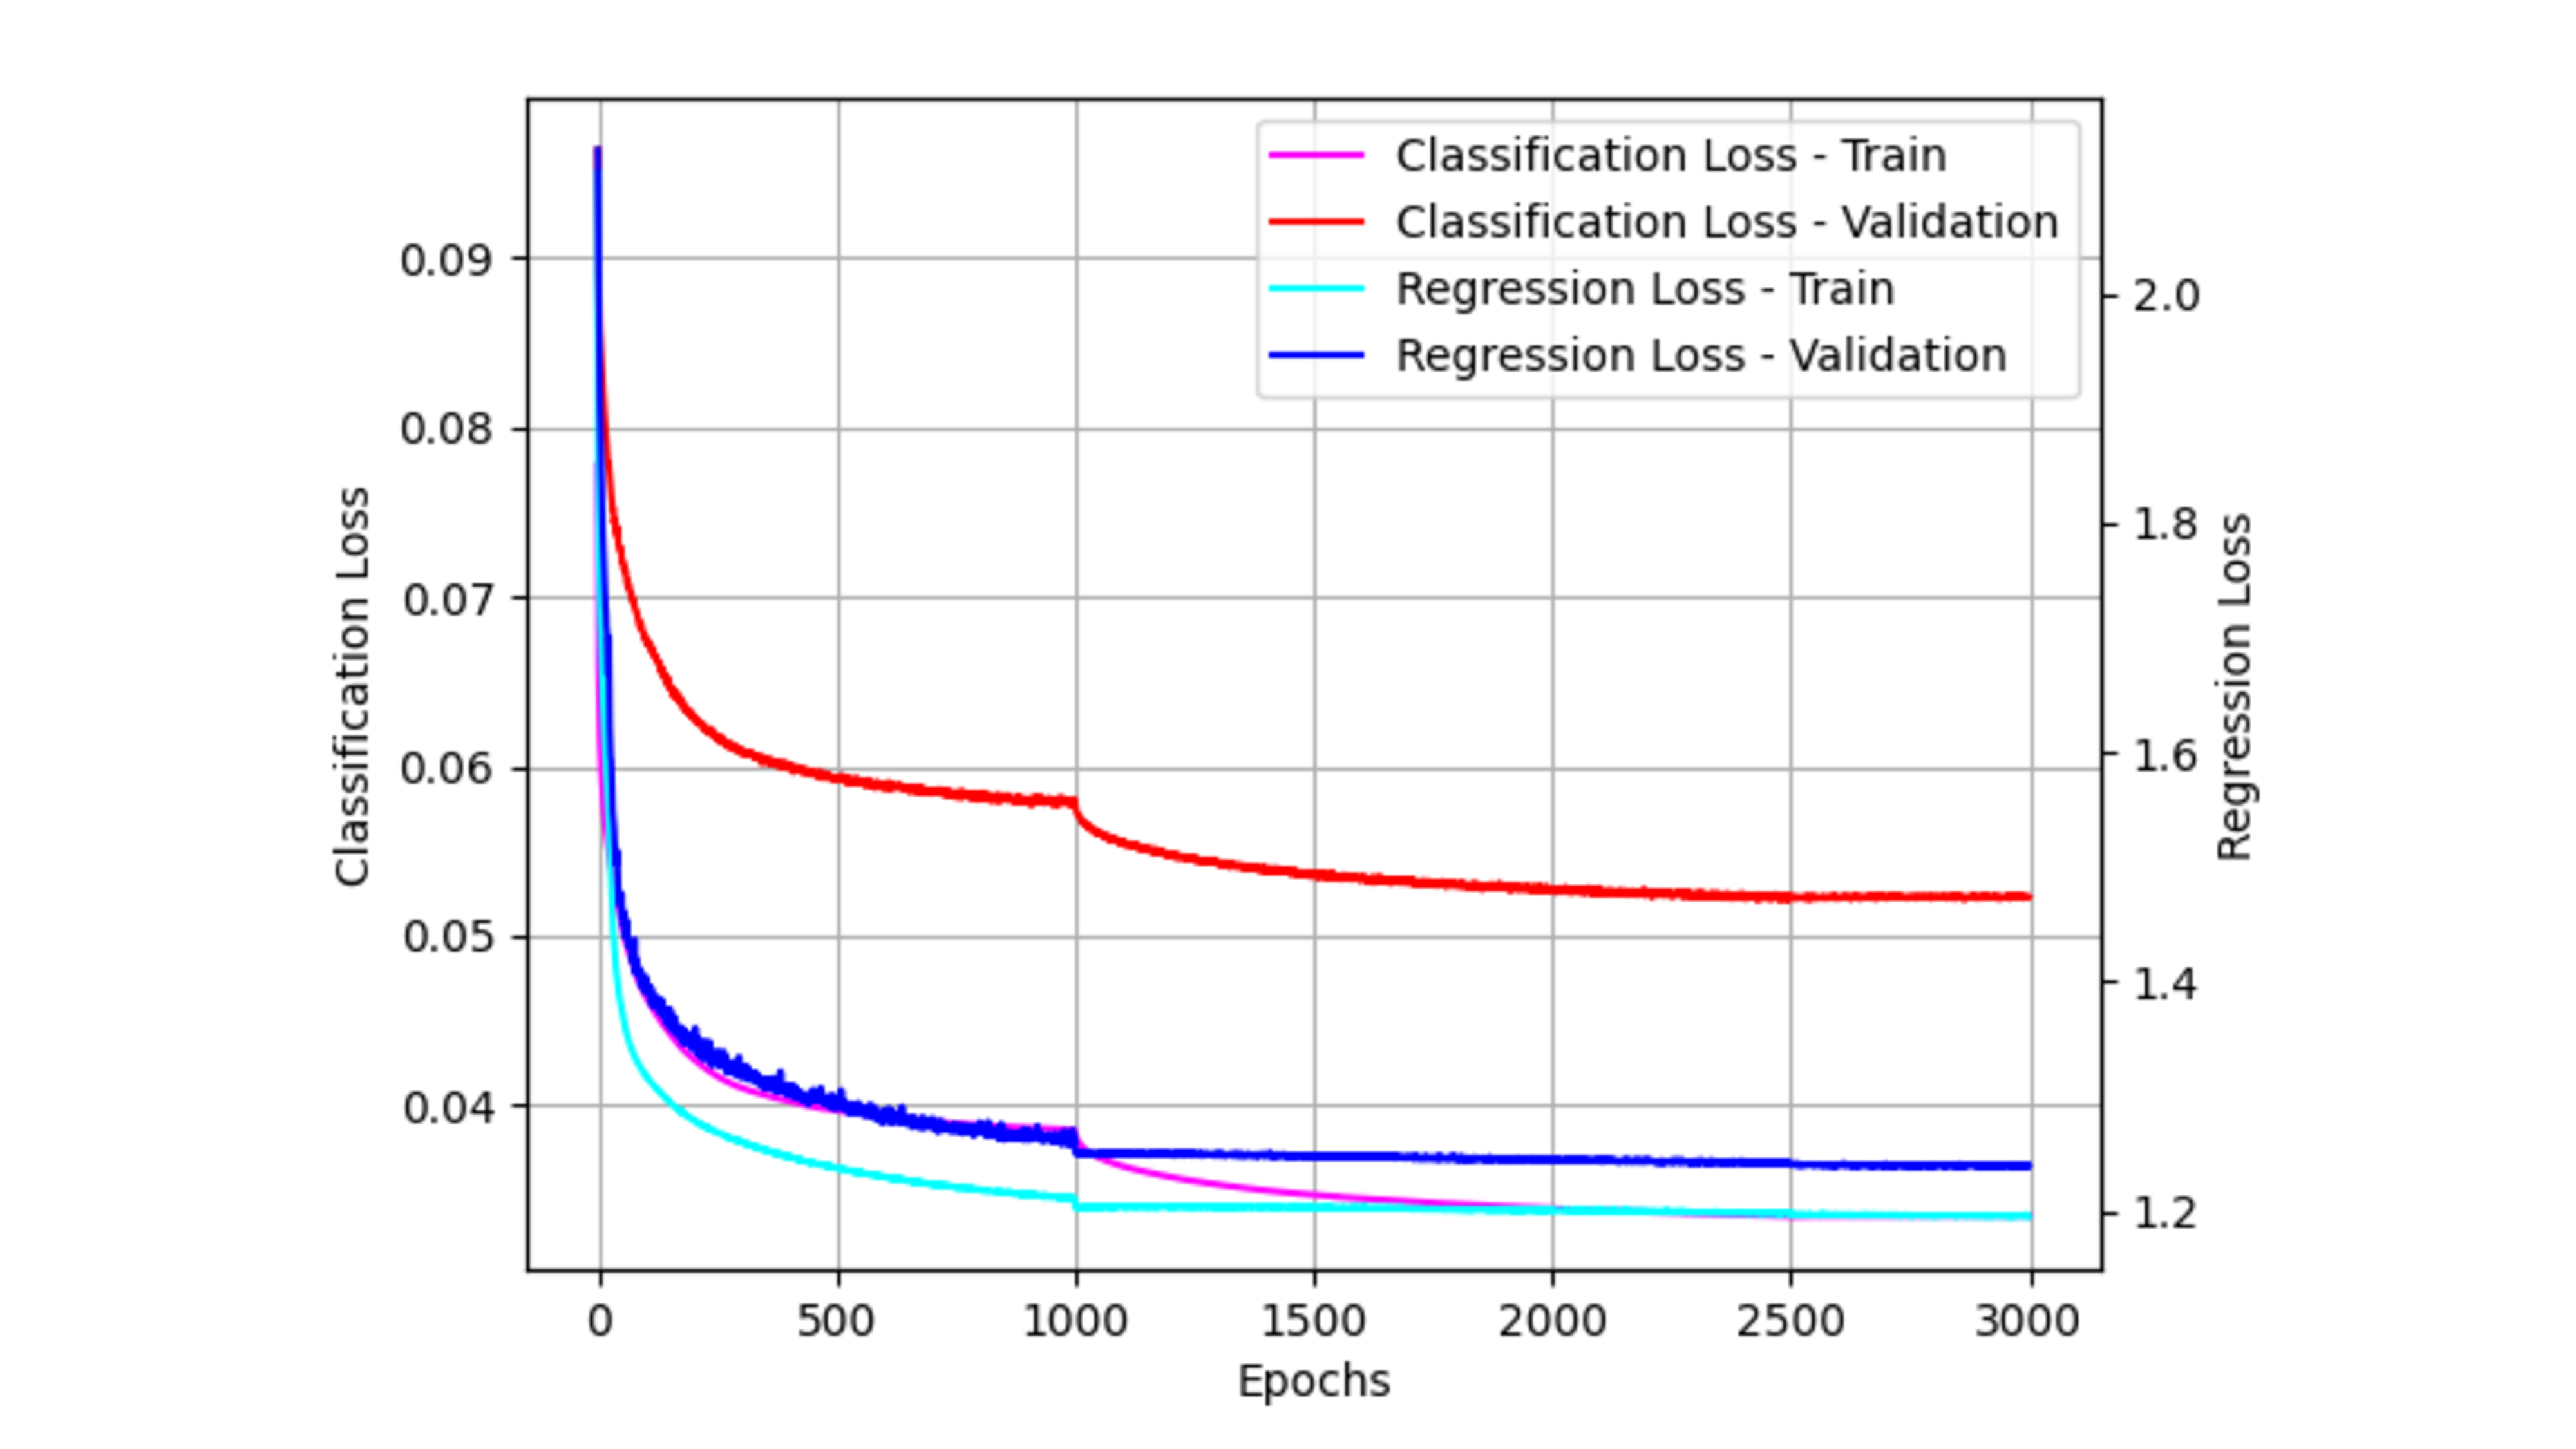
\includegraphics[width=1.0\textwidth]{Figure/3Networks/3-3-2-2TrainingCurve.png}
 %\caption{飛跡対についてのネットワークの学習曲線}
 %\label{3-3-2-2TrainingCurve}
%\end{figure}


%%%%%%%%%%%%%%%%%%%%%%%%%%%%%%%%%%%%%%%%%%%%%%%%%%%%%%%%%%%%%%%%%%%%%%%%
\subsection{ネットワークの性能} \label{Net:PM:PerformanceofPM}

ここではネットワークの性能を評価する。

まず、ネットワークがどの変数を見ているかについて評価する。
ここでは、崩壊点の位置とトラック・パラメータの共分散行列について調査を行う。
崩壊点を分類する上で崩壊点の位置についての情報は非常に重要である。
特に各Secondary Vertexを識別するためにネットワークは、トラック・パラメータから粒子の飛跡を再構成し、それらが交点を持つかを評価する必要がある。
また、ネットワークに誤差などの情報を取り入れることは困難であると言われており、本研究においても、ネットワークが共分散行列の情報を取り扱えているかを評価せねばならないと考える。

そのため、図\ref{3-3-3-1PairModels}のようなネットワーク、モデルA・モデルB・モデルC・モデルDを構築する。
モデルAとモデルDは図\ref{3-3-1-1PairModel}と同様の構造である。
モデルAでは飛跡についての全ての情報を使用し、モデルDでは共分散行列を取り除いた14個の変数を使用する。
モデルBはLCFIPlusで計算された崩壊点の位置を出力の直前の全結合層に使用している。
モデルBでは、訓練データの正解ラベルであるLCFIPlusで計算された崩壊点の位置を入力として使用しているため、出力は崩壊点の分類のみとしている。
モデルCはネットワークで予想された崩壊点の位置を出力の直前の全結合層に使用している。

\begin{figure}[htbp]
 \centering
  %\begin{tabular}{cccc}
  \begin{minipage}{1.0\textwidth}
  \centering
   \begin{minipage}{0.48\textwidth}
    \centering
    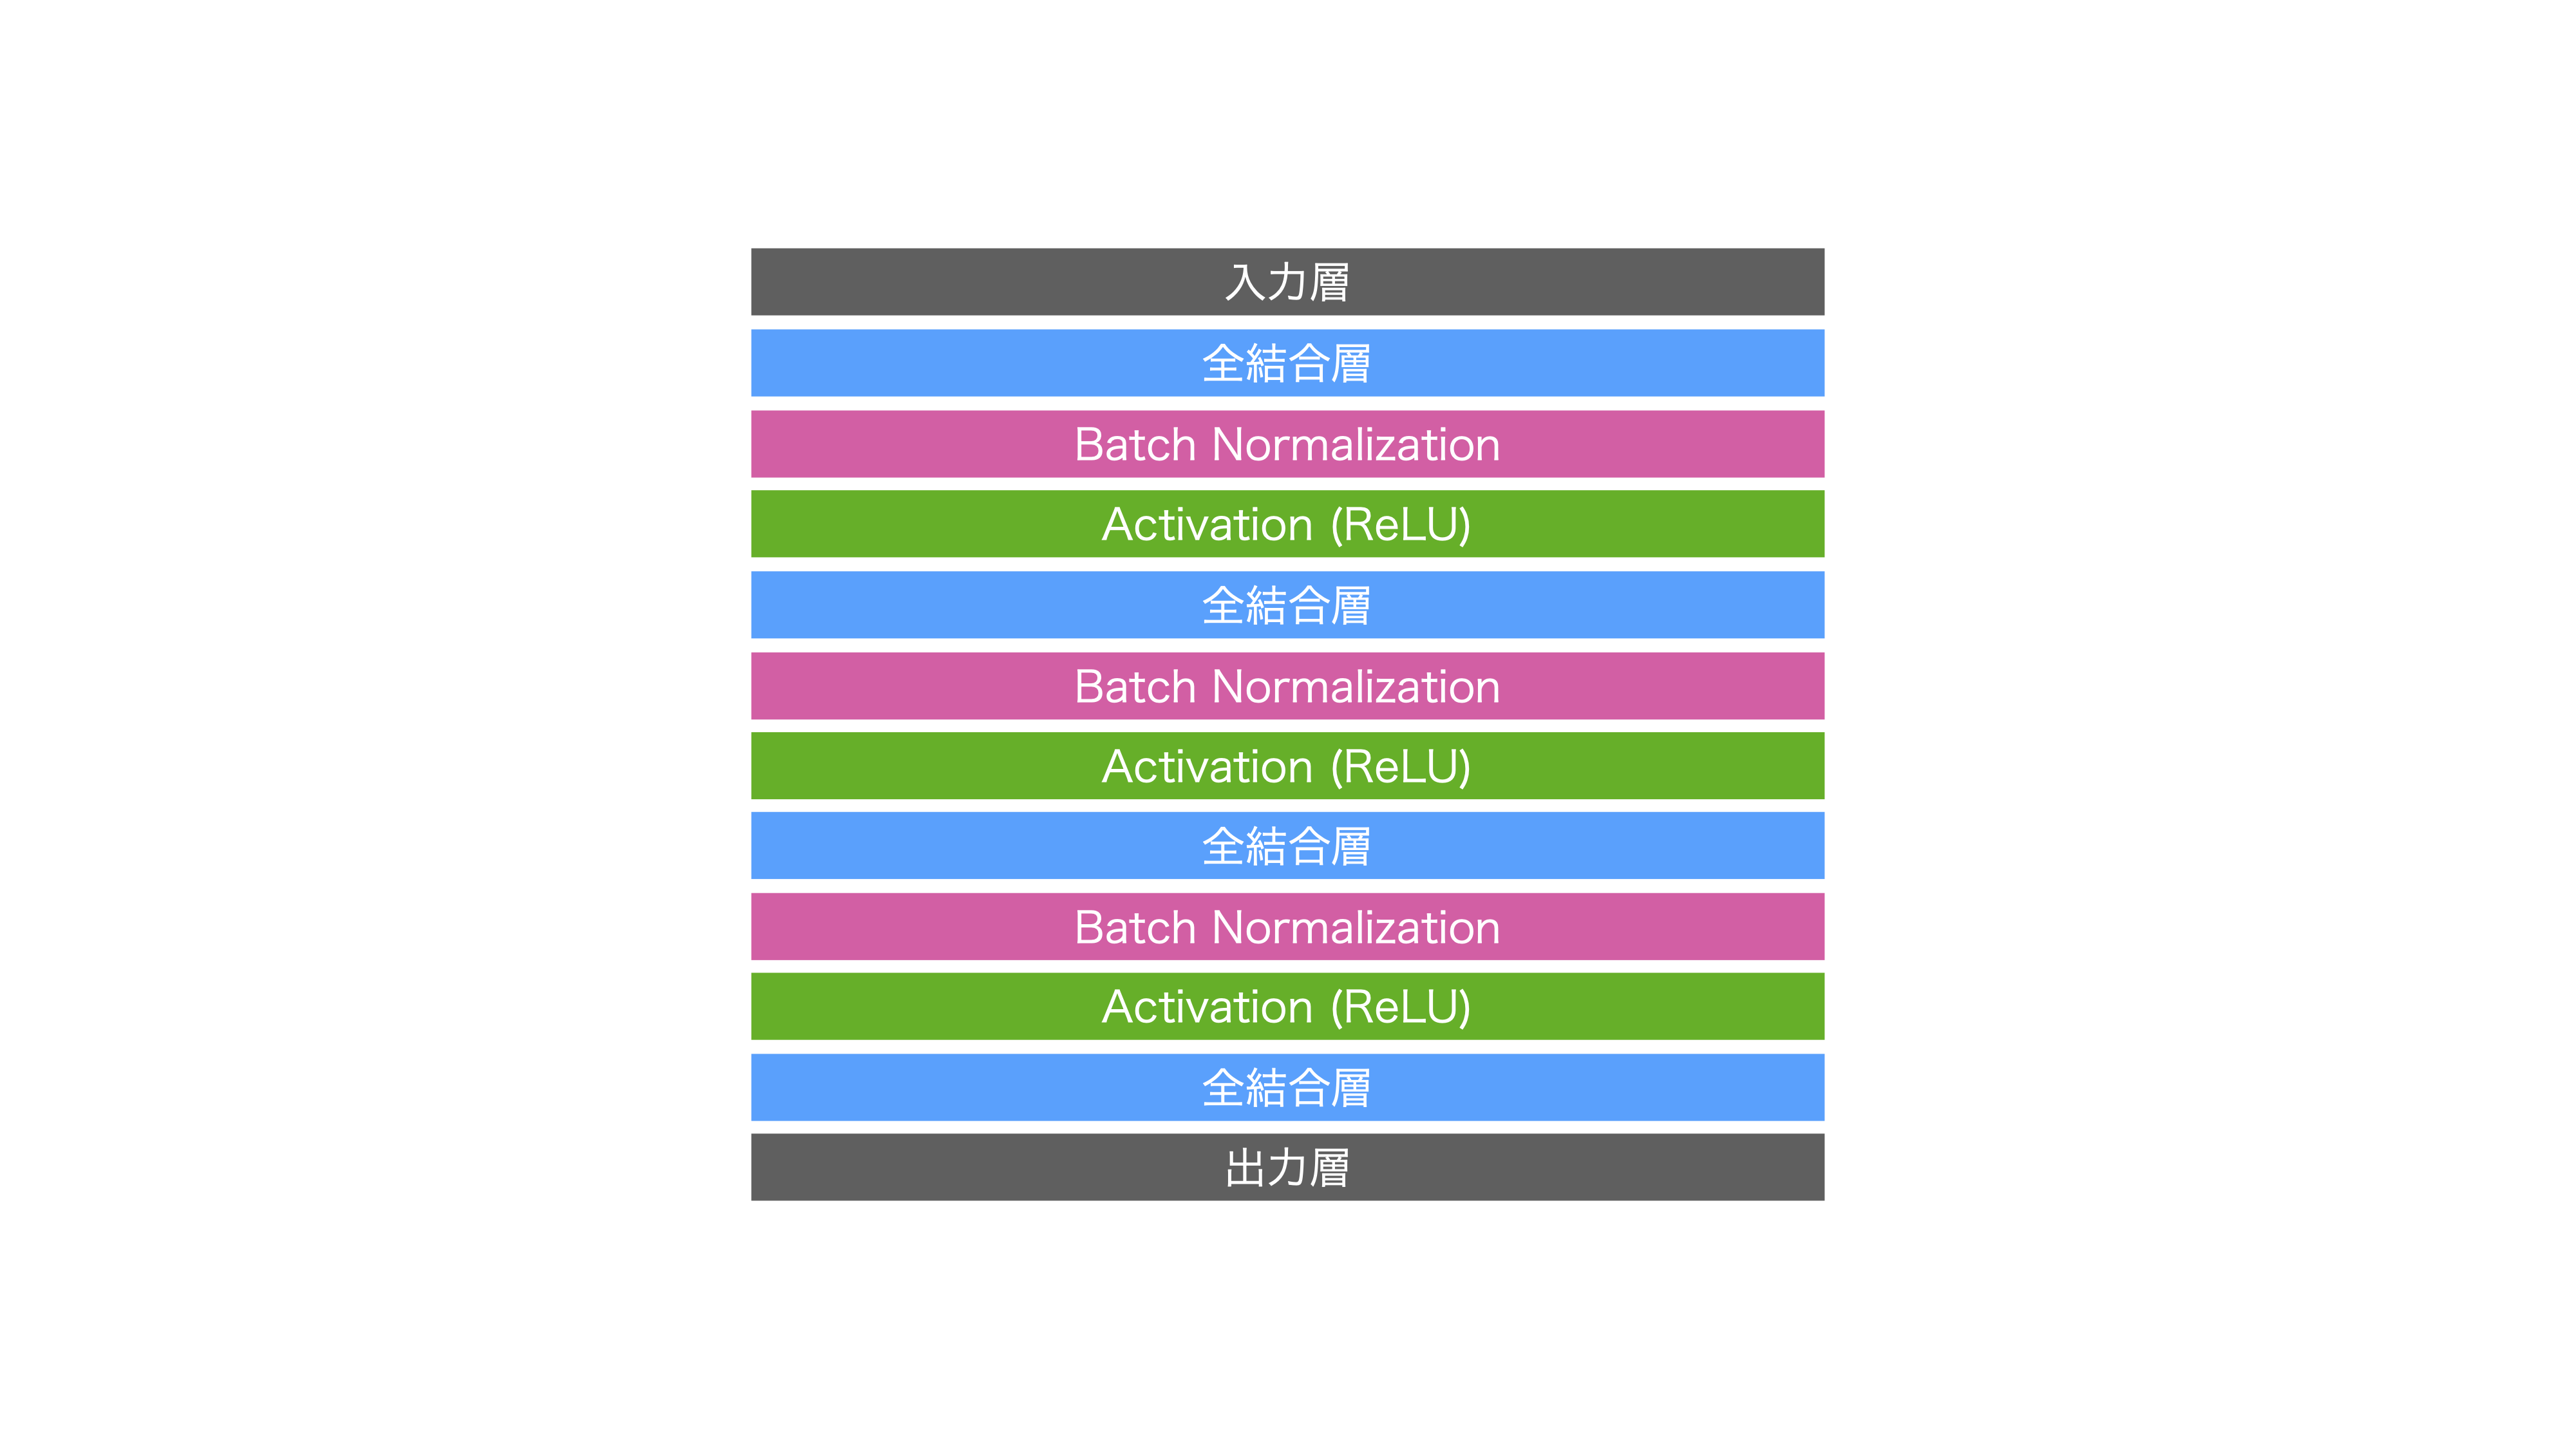
\includegraphics[trim = 200 0 200 0, width=1.0\textwidth, clip]{Figure/3Networks/3-3-1-1PairModel.png}
    \subcaption{モデルA}
   \end{minipage}
   \begin{minipage}{0.48\textwidth}
   \centering
    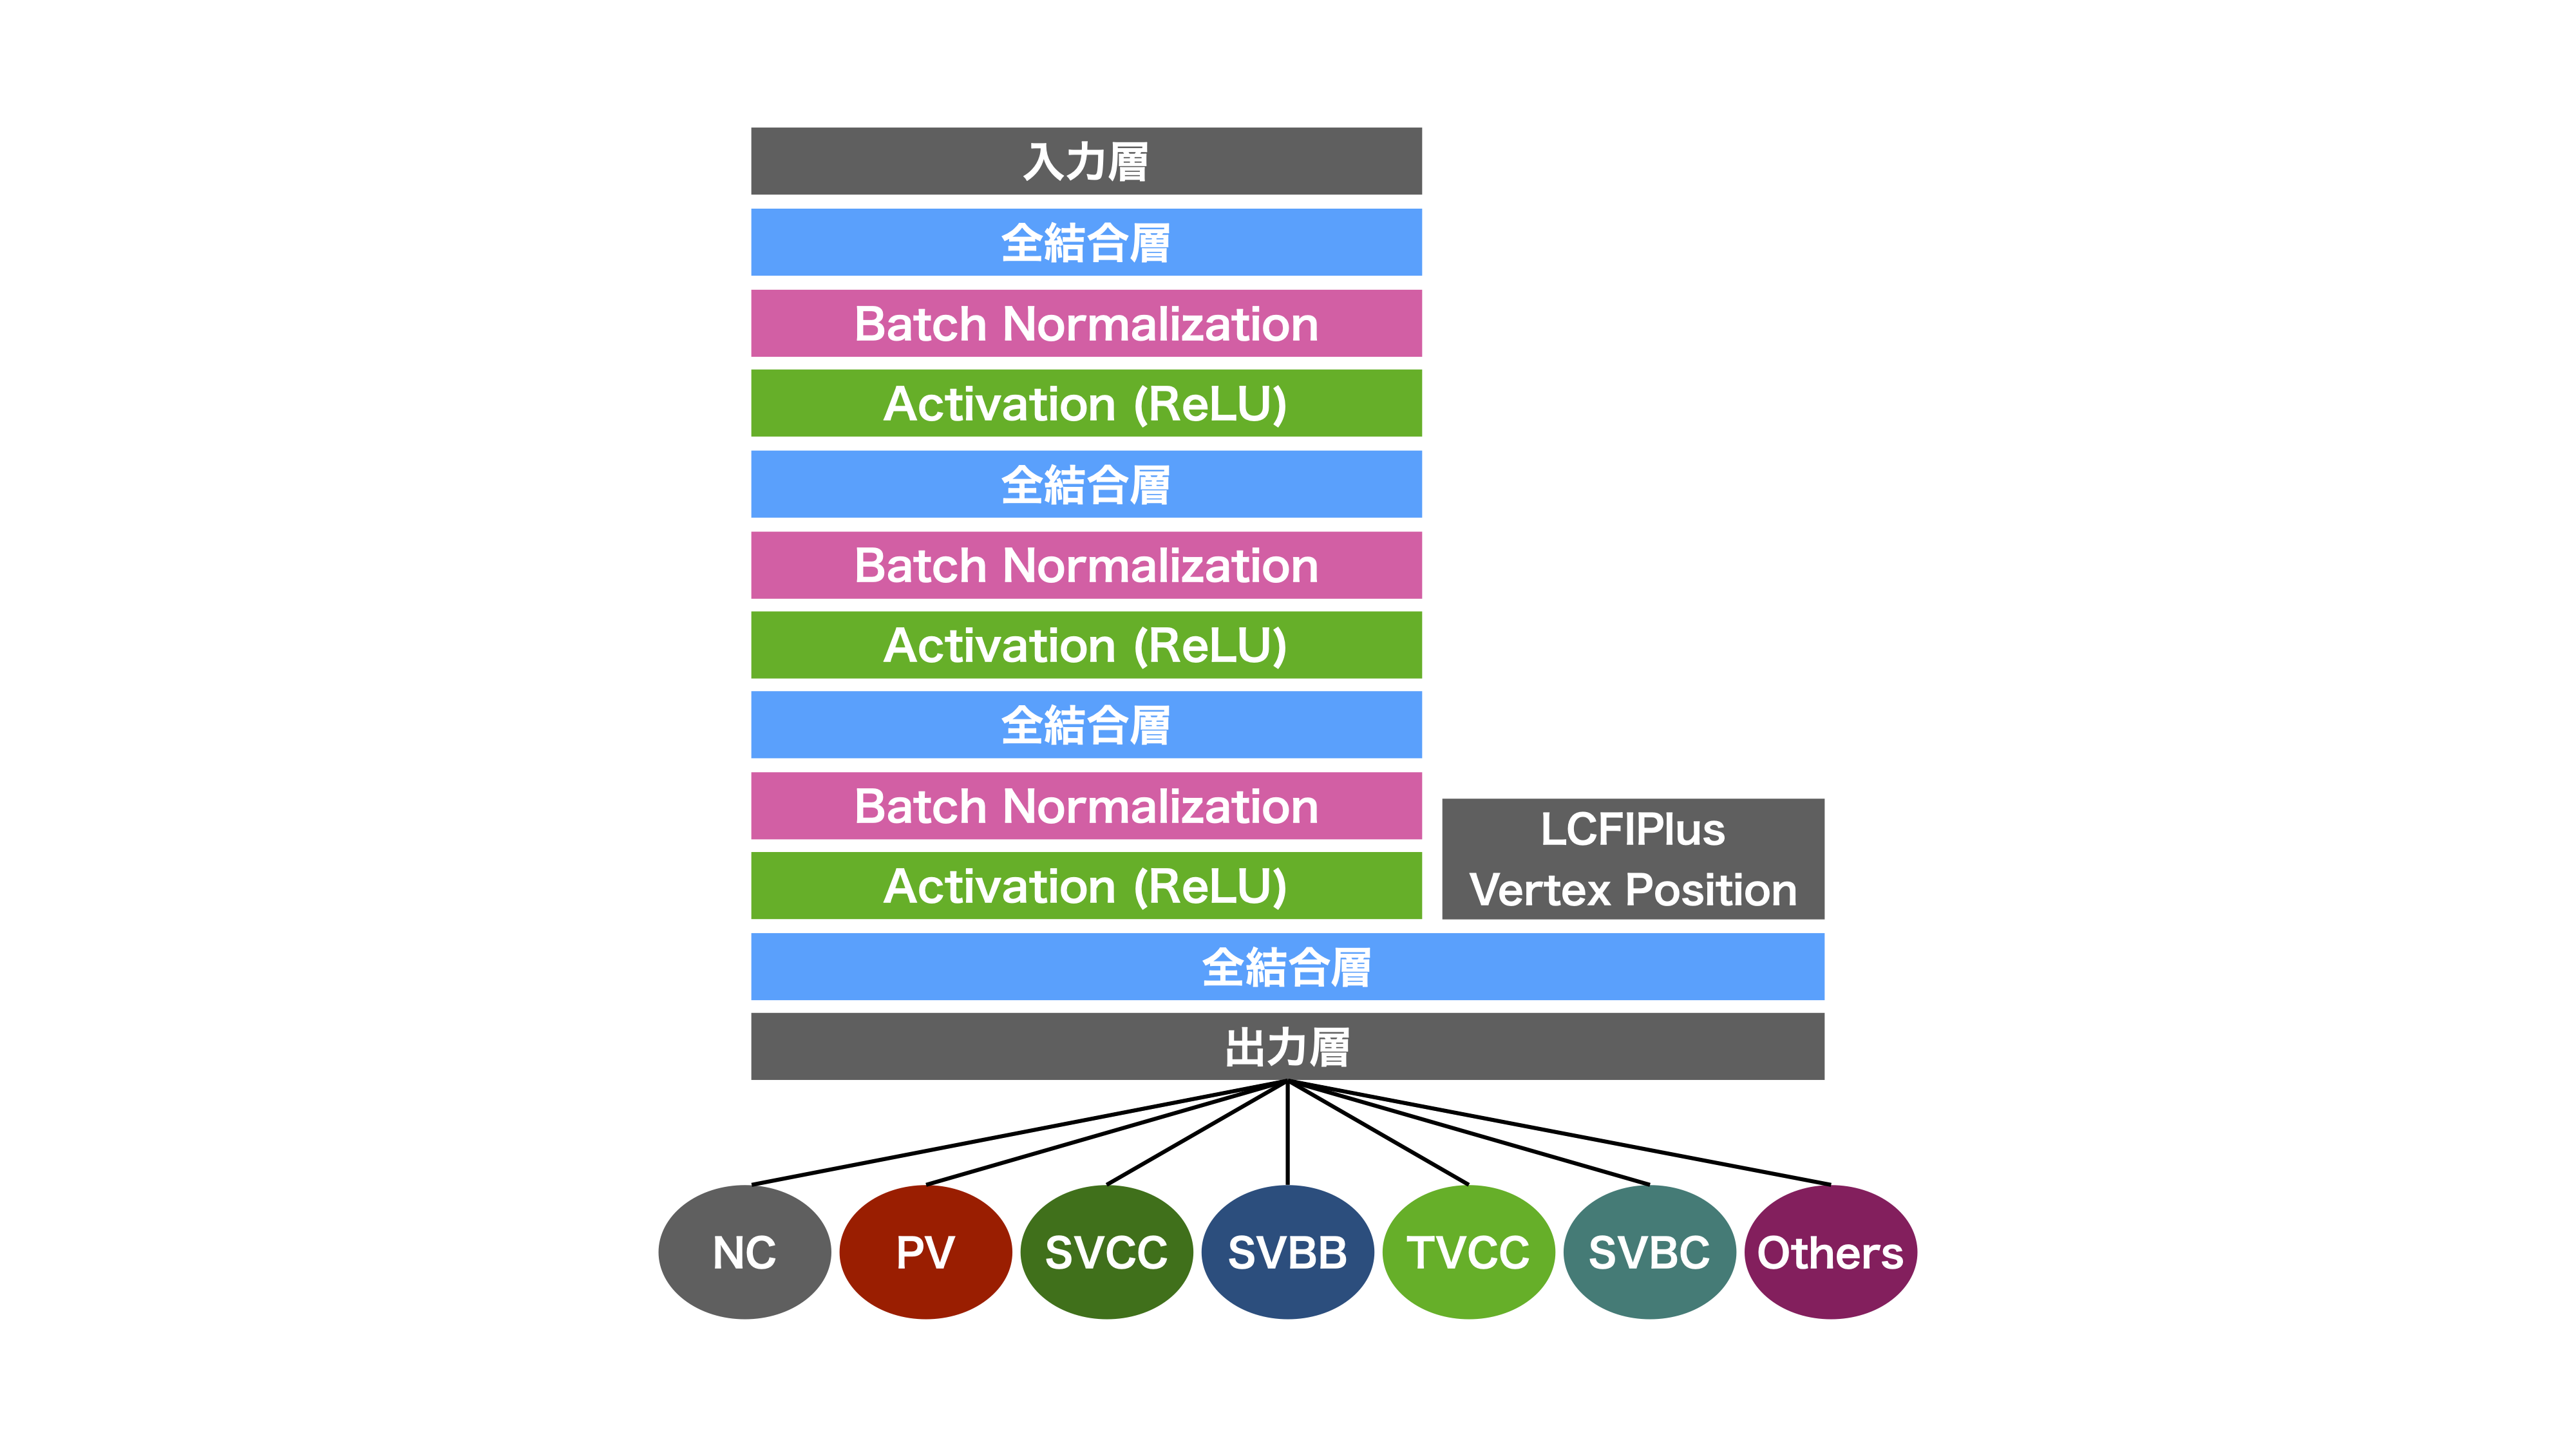
\includegraphics[trim = 200 0 200 0, width=1.0\textwidth, clip]{Figure/3Networks/3-3-3-1PairModelB.png}
    \subcaption{モデルB}
    \label{3-3-3-1PairModelB}
   \end{minipage}
  \end{minipage}  

  \begin{minipage}{1.0\textwidth}
  \centering
   \begin{minipage}{0.48\textwidth}
   \centering
    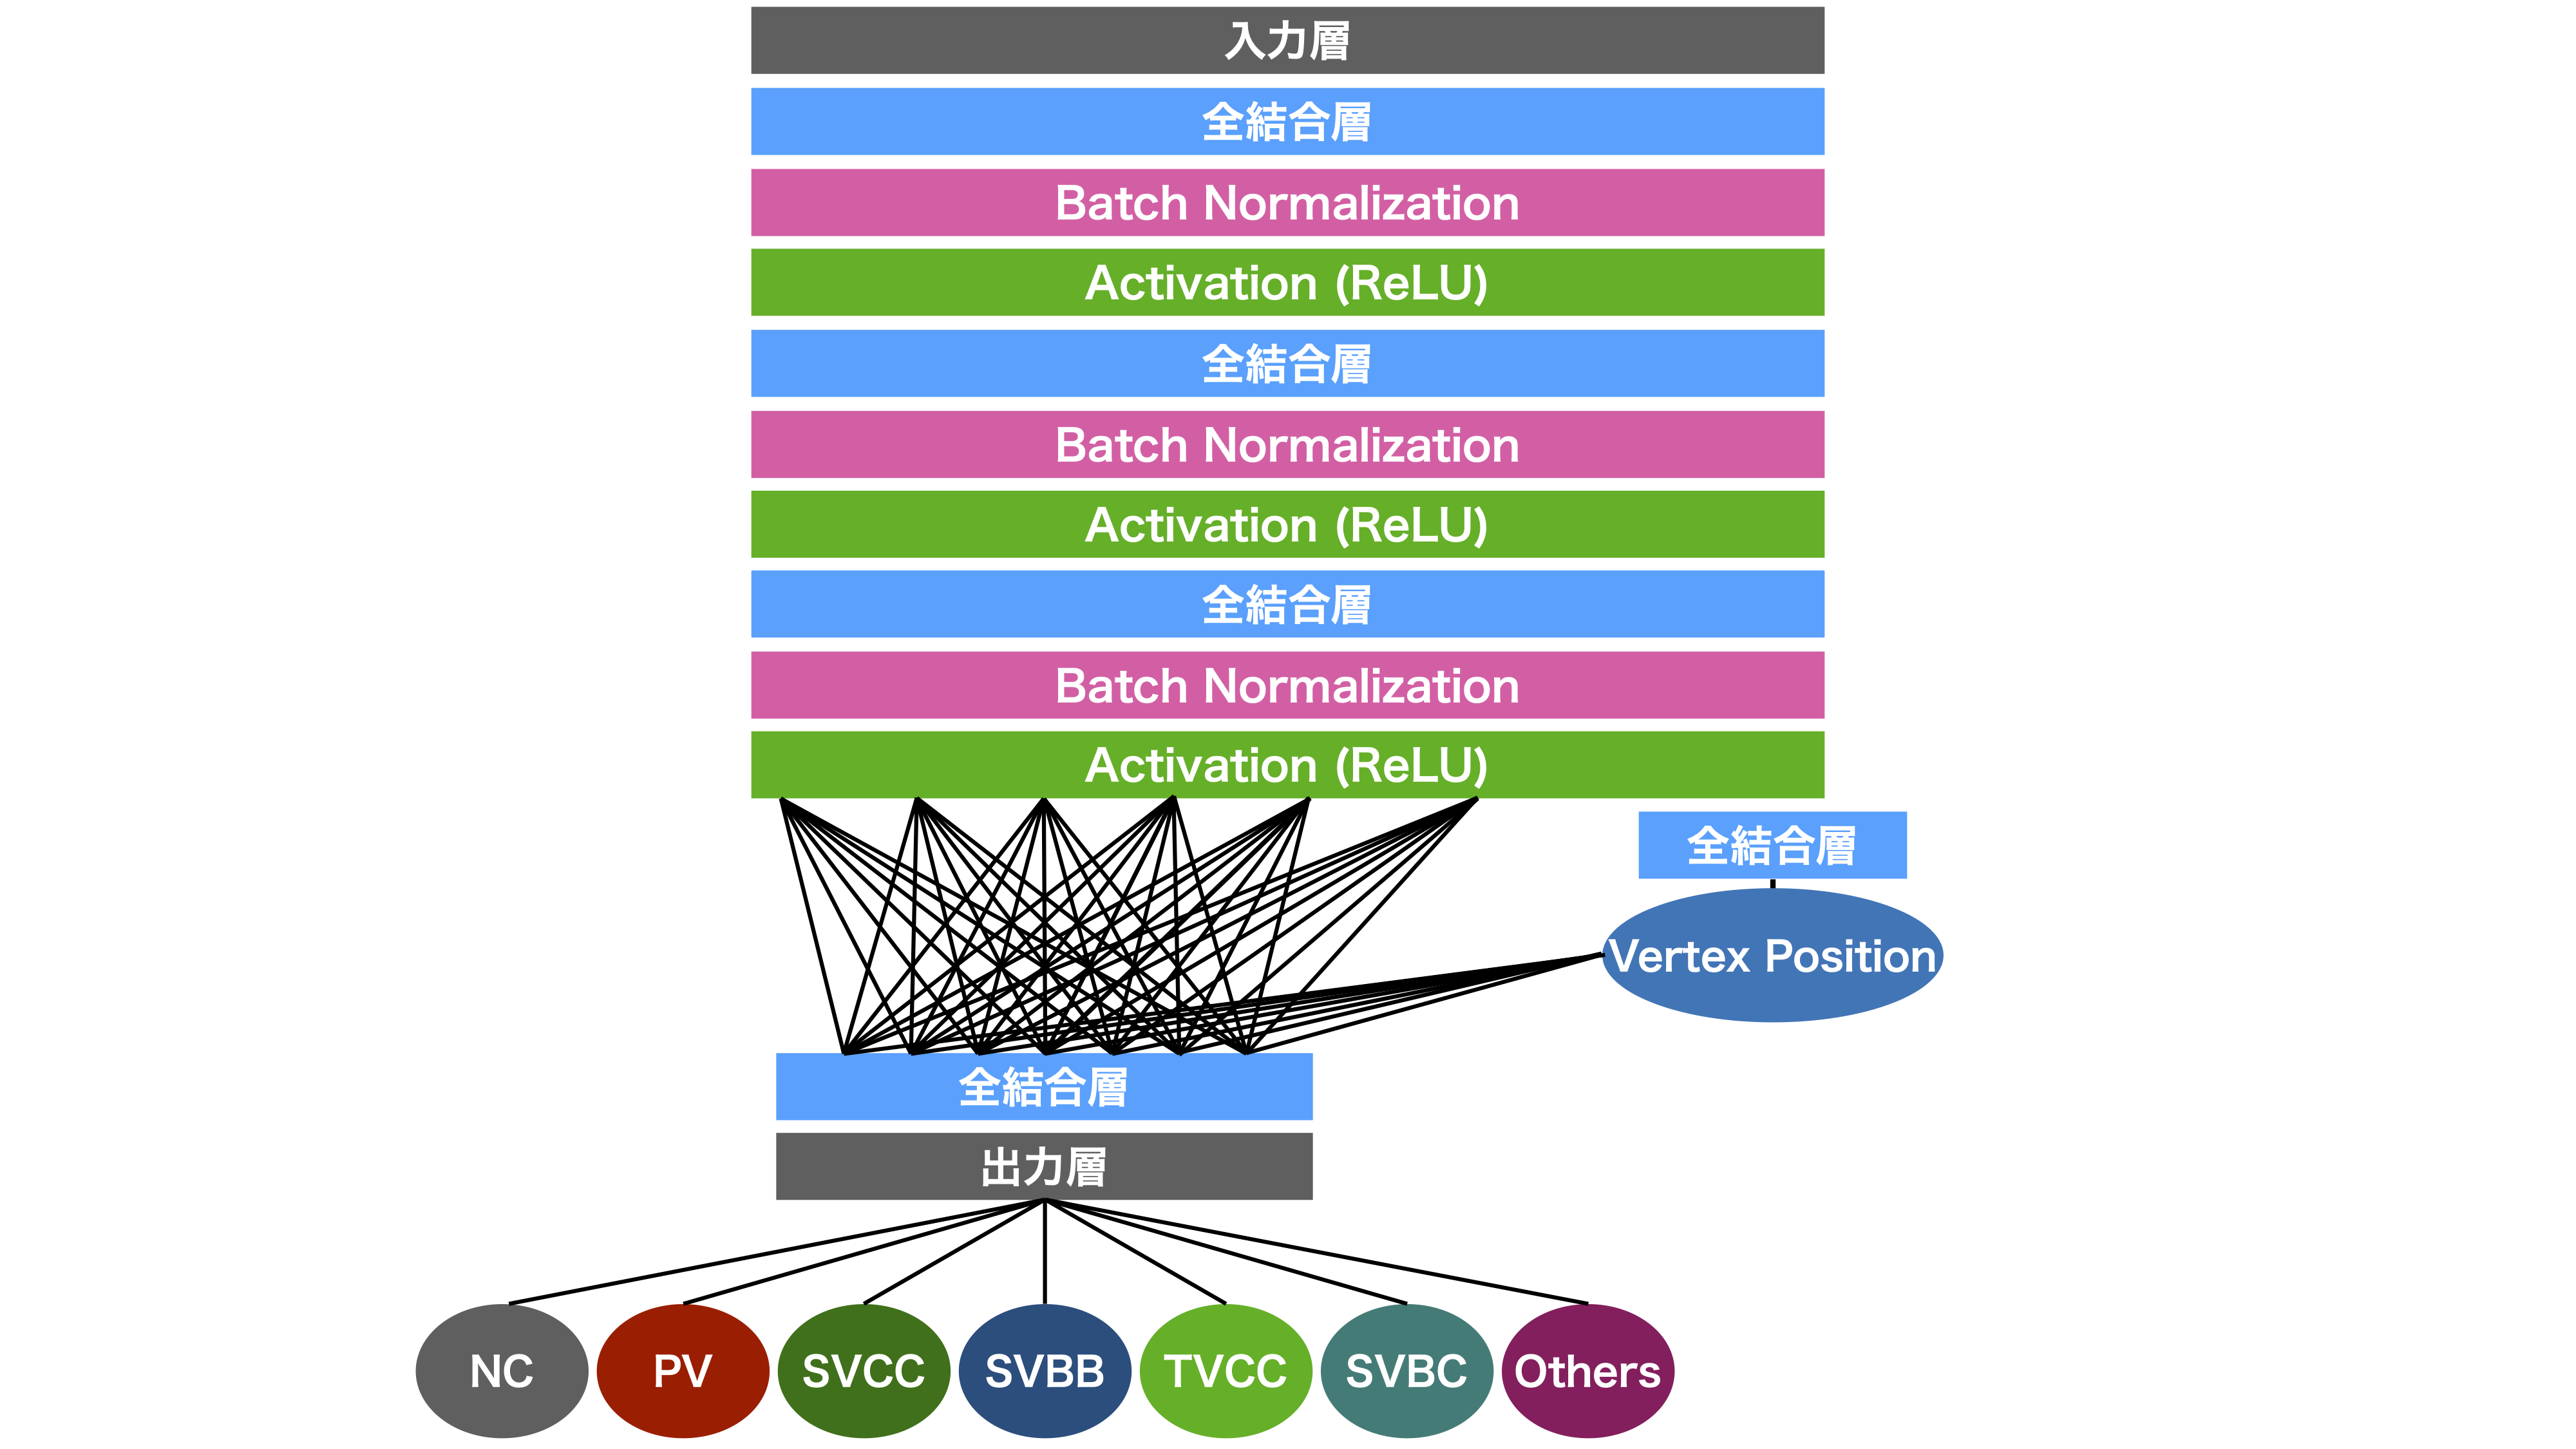
\includegraphics[trim = 200 0 200 0, width=1.0\textwidth, clip]{Figure/3Networks/3-3-3-1PairModelC.png}
    \subcaption{モデルC}
    \label{3-3-3-1PairModelC}
   \end{minipage}
   \begin{minipage}{0.48\textwidth}
   \centering
    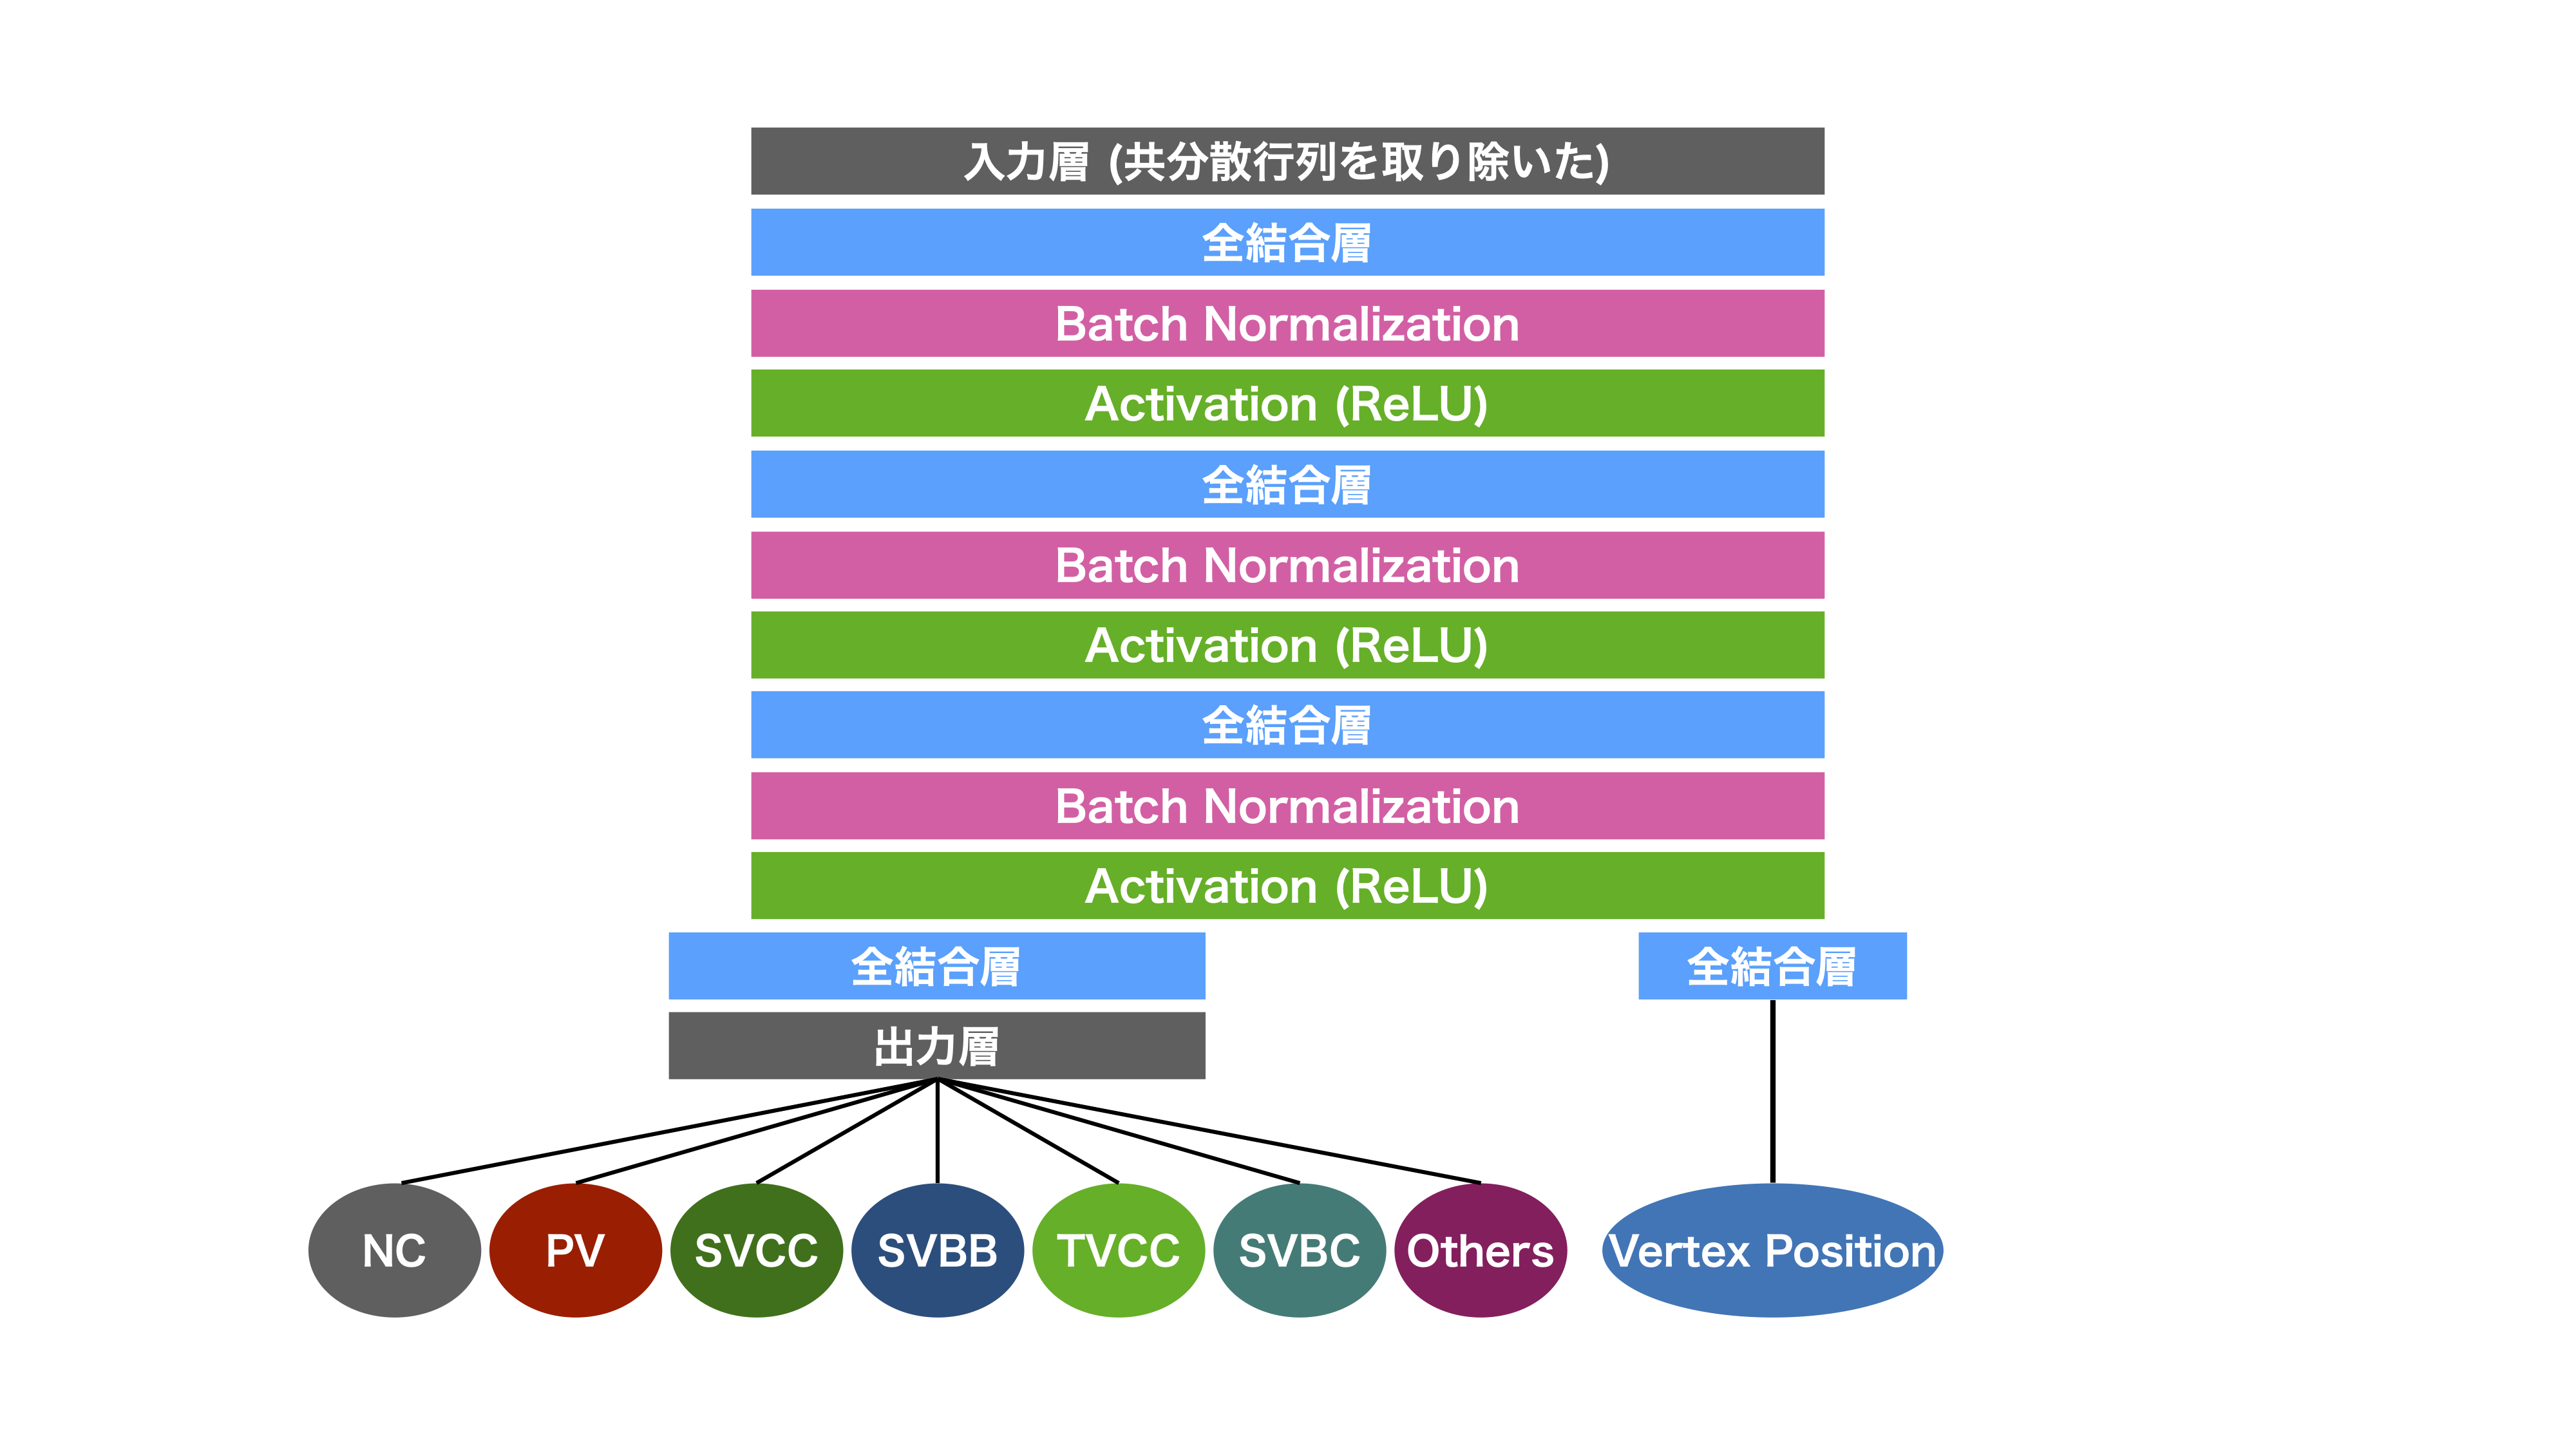
\includegraphics[trim = 200 0 200 0, width=1.0\textwidth, clip]{Figure/3Networks/3-3-3-1PairModelD.png}
    \subcaption{モデルD}
    \label{3-3-3-1PairModelD}
   \end{minipage}
   \end{minipage}
  \caption{評価のための飛跡対についてのネットワーク}
  \label{3-3-3-1PairModels}
 %\end{tabular}
\end{figure}

これらのネットワークの性能は混合行列を用いて評価する。
特にここでは、効率と純度についての混合行列を作成した。
また、出力として崩壊点の位置を予想するネットワークに関しては崩壊点の位置についての損失を用いて評価を行う。

\begin{figure}[htbp]
 \centering
  %\begin{tabular}{cccc}
   \begin{minipage}{1.0\textwidth}
    \centering
    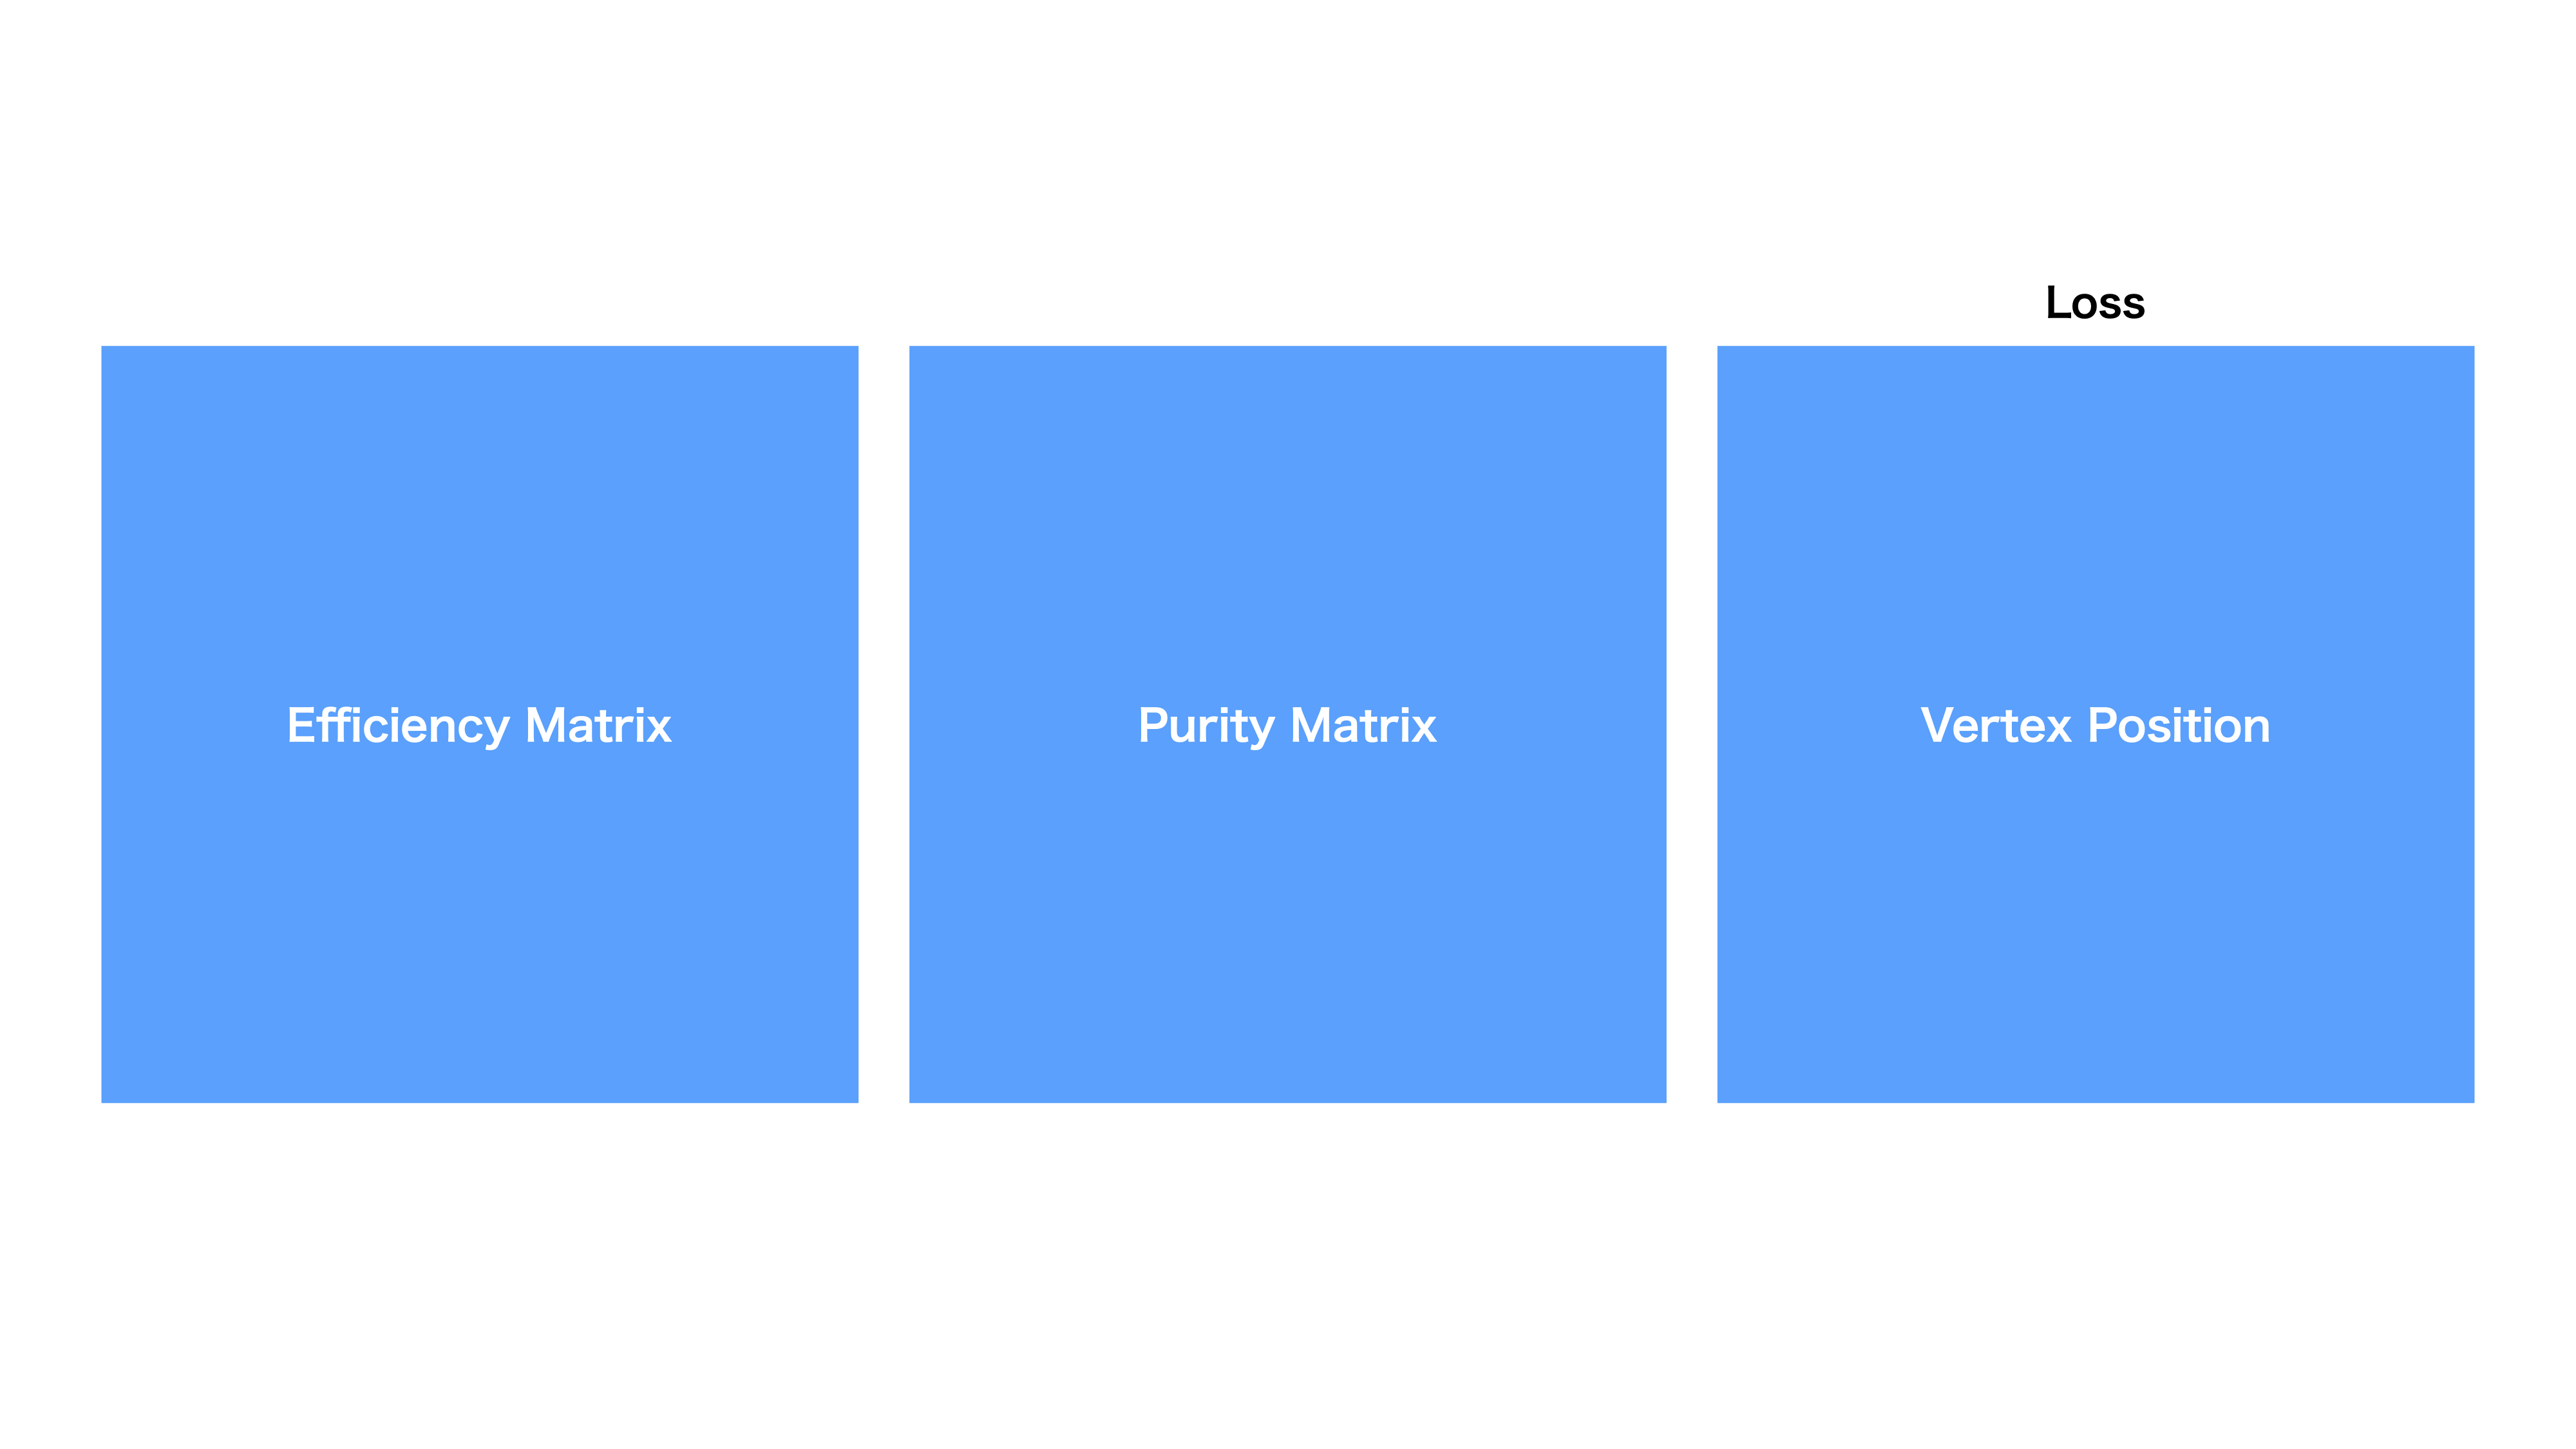
\includegraphics[trim = 0 220 0 220, width=0.9\textwidth, clip]{Figure/3Networks/3-3-3-2ConfusionMatrixA.png}
    \subcaption{モデルAの混合行列と崩壊点の位置}
    \label{3-3-3-2ConfusionMatrixA}
   \end{minipage}

   \begin{minipage}{1.0\textwidth}
   \centering
    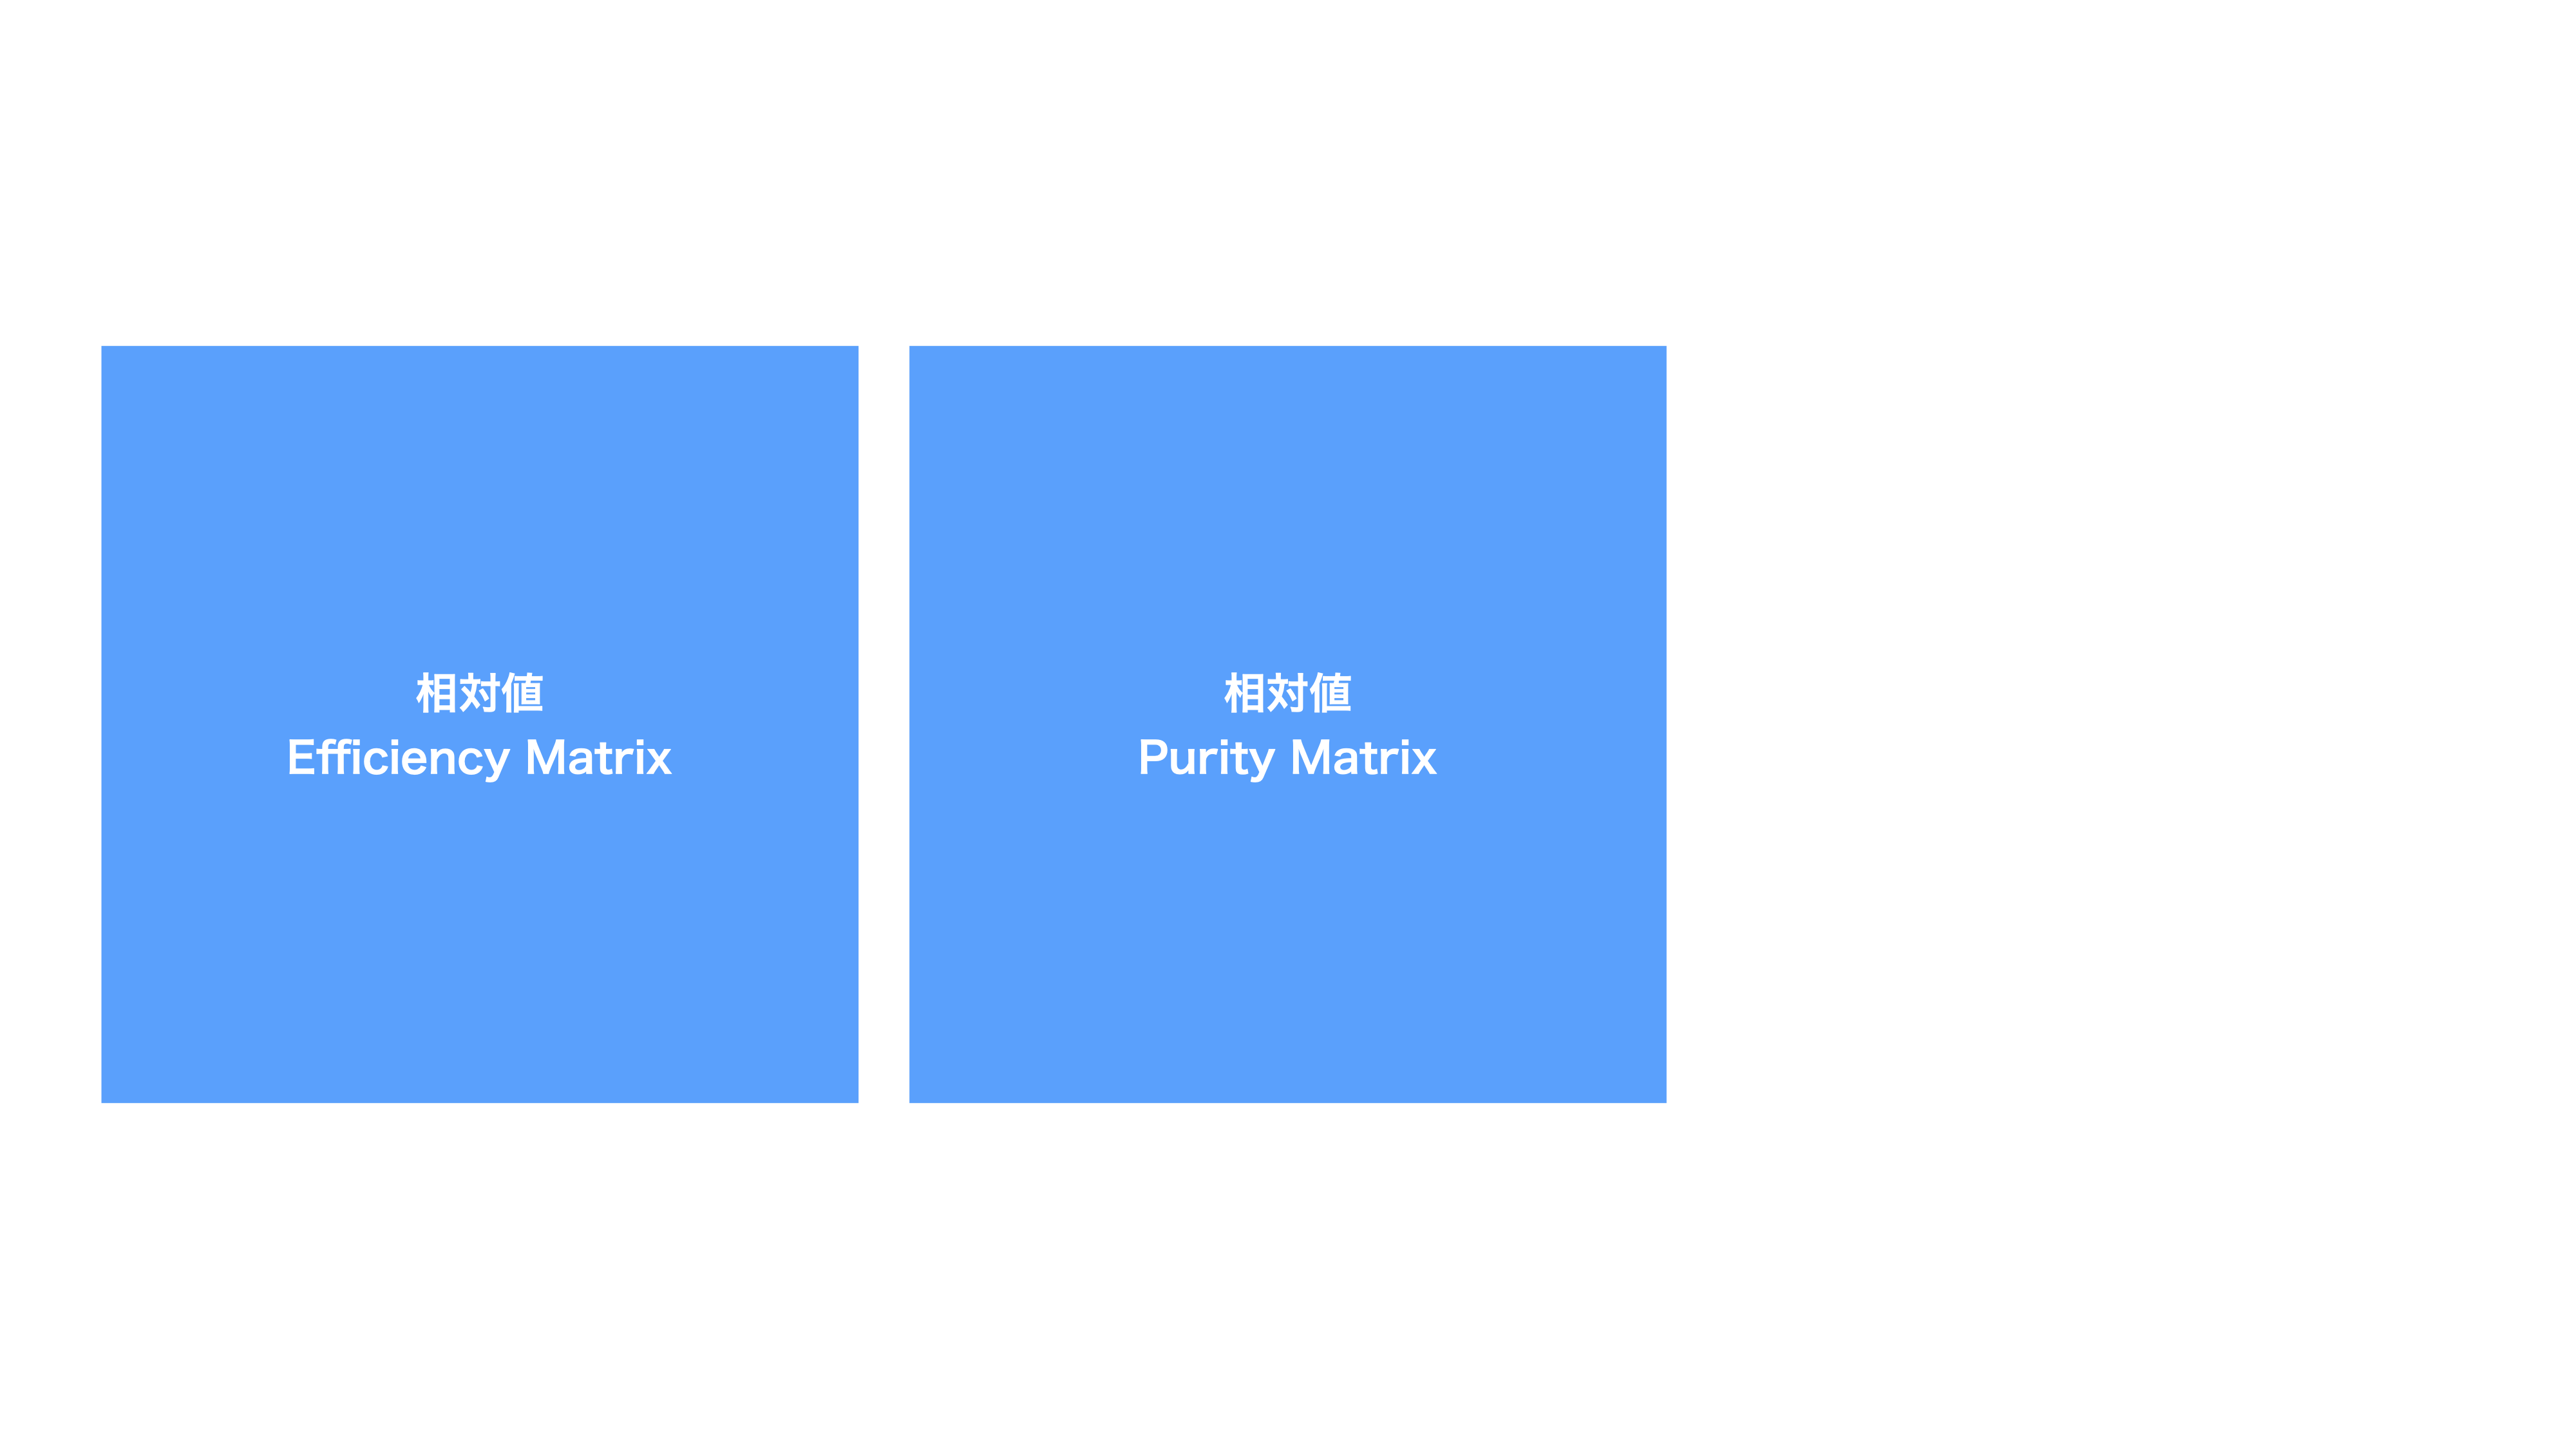
\includegraphics[trim = 0 220 0 220, width=0.9\textwidth, clip]{Figure/3Networks/3-3-3-2ConfusionMatrixB.png}
    \subcaption{モデルBの混合行列の相対値}
    \label{3-3-3-2ConfusionMatrixB}
   \end{minipage}
  
  \begin{minipage}{1.0\textwidth}
   \centering
    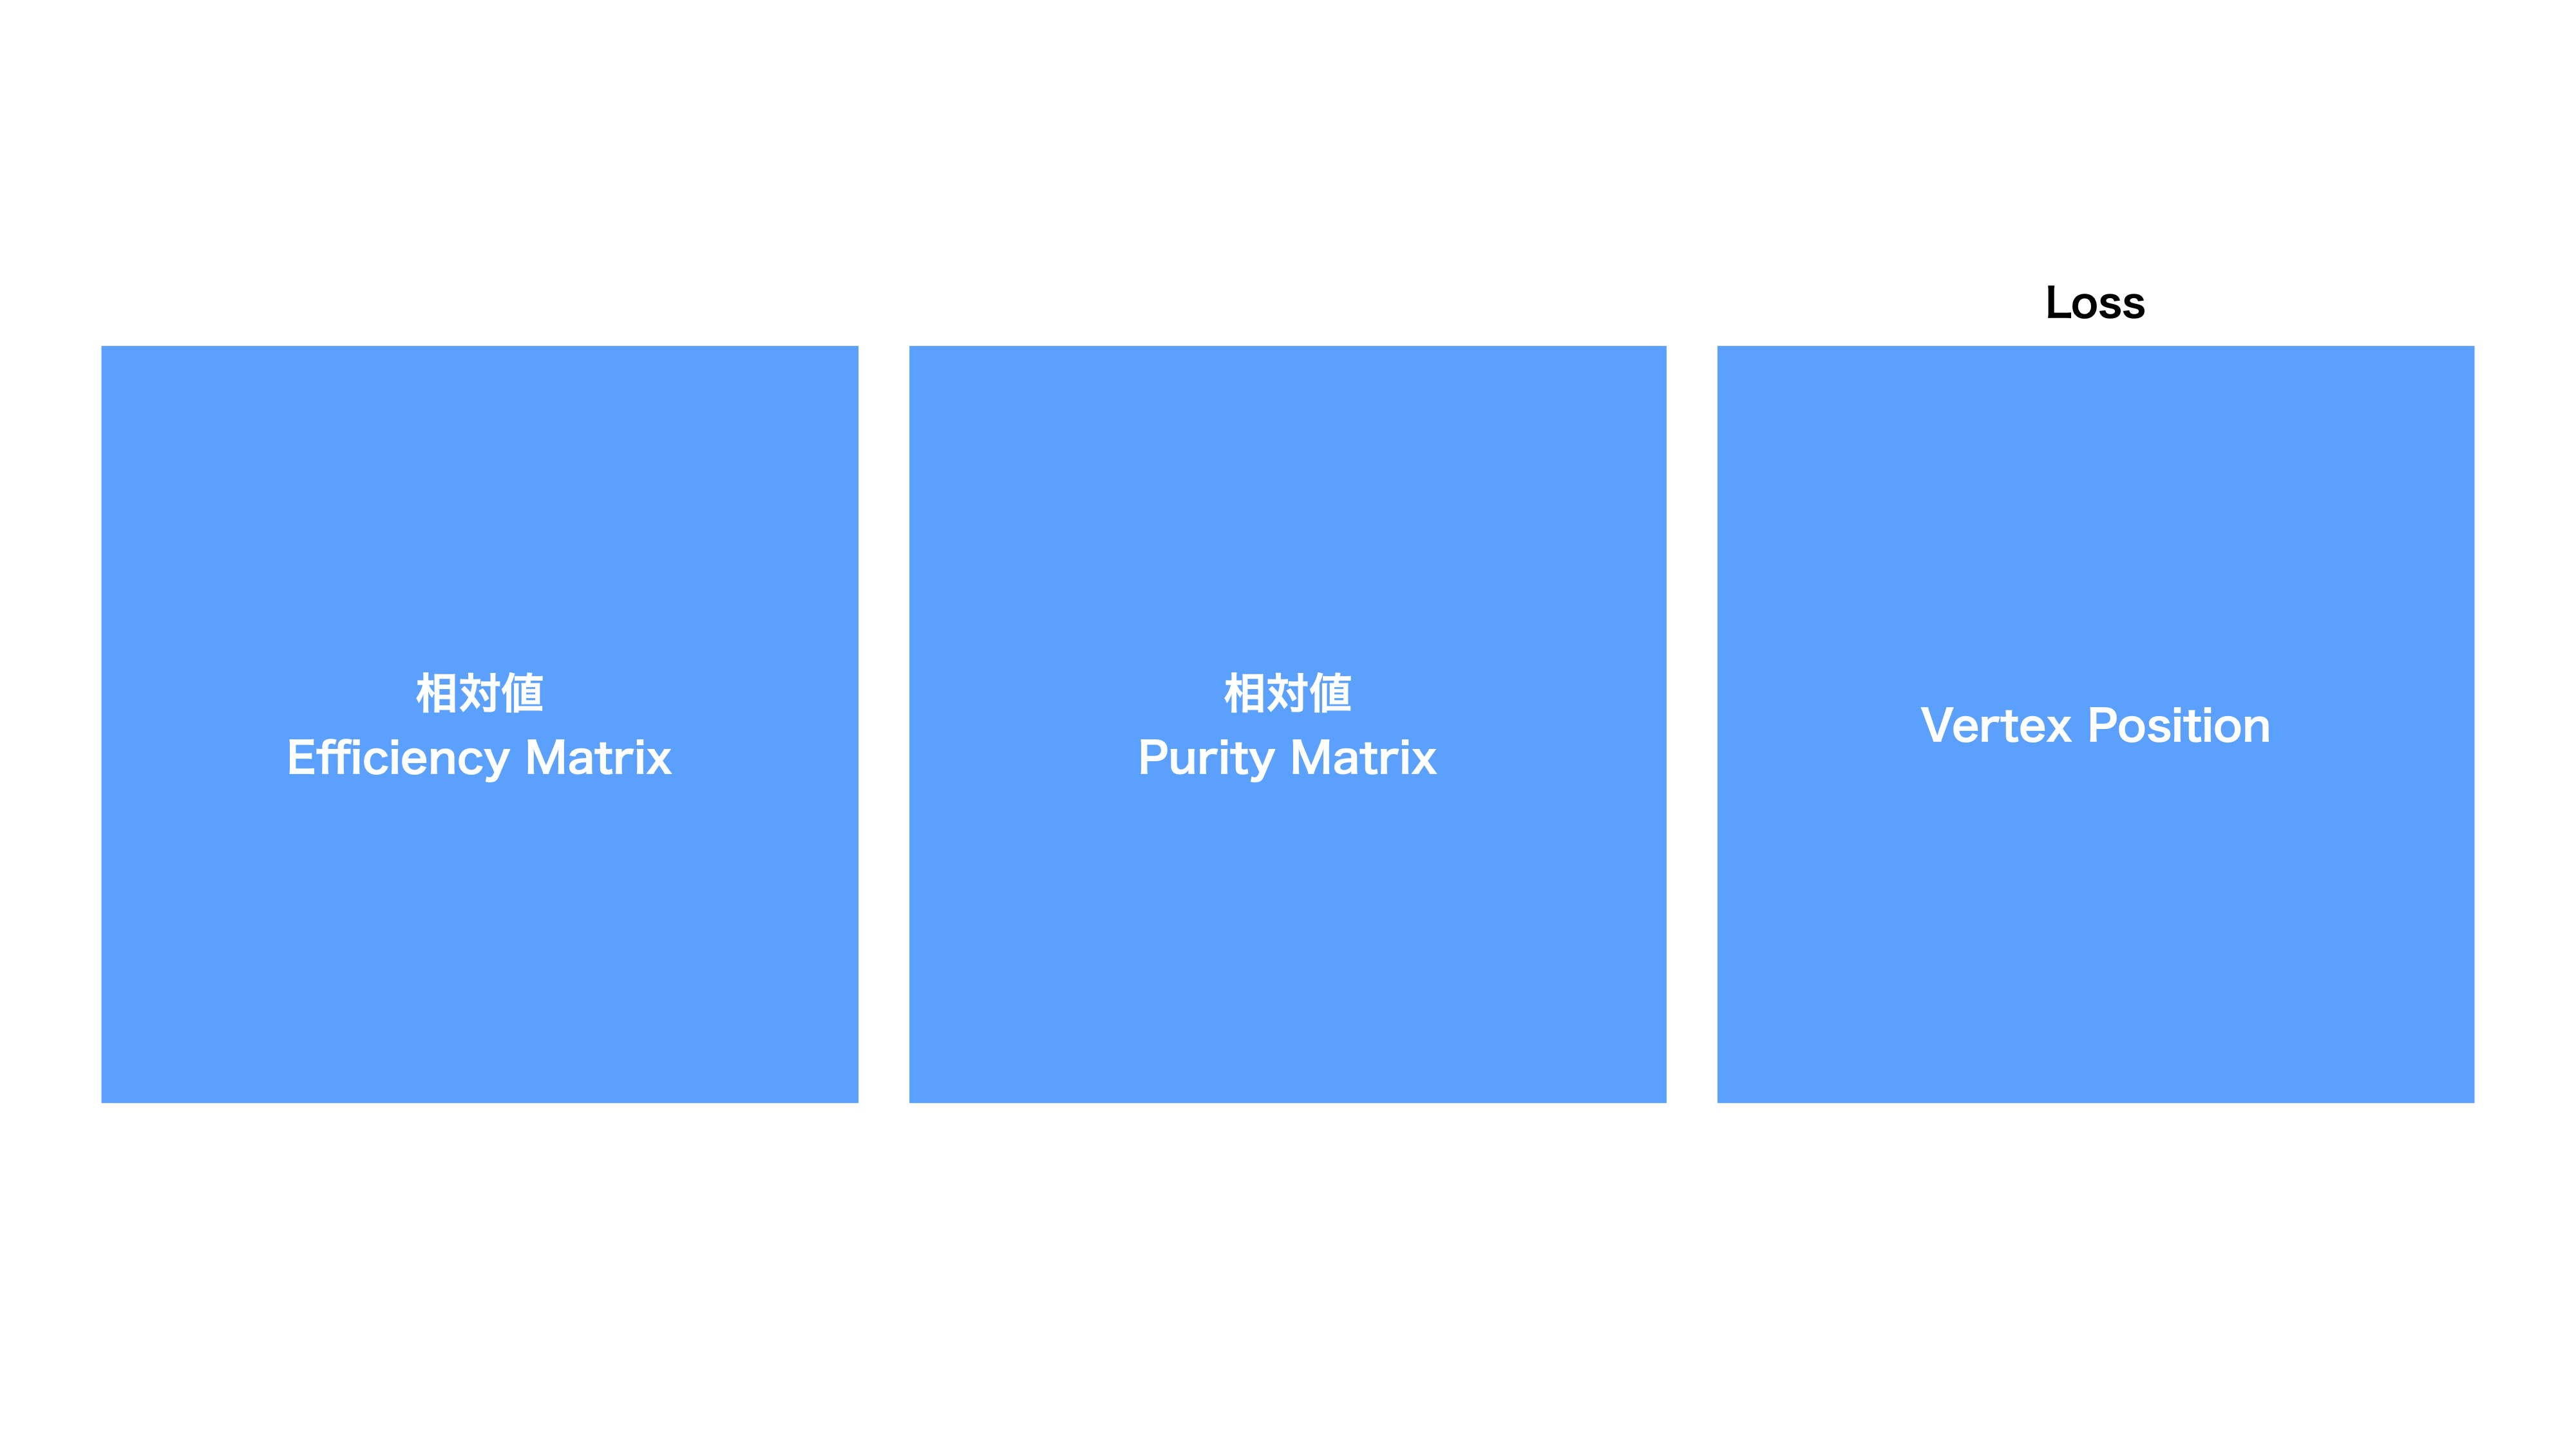
\includegraphics[trim = 0 220 0 220, width=0.9\textwidth, clip]{Figure/3Networks/3-3-3-2ConfusionMatrixC.png}
    \subcaption{モデルCの混合行列の相対値と崩壊点の位置}
    \label{3-3-3-2ConfusionMatrixC}
   \end{minipage}
   
   \begin{minipage}{1.0\textwidth}
   \centering
    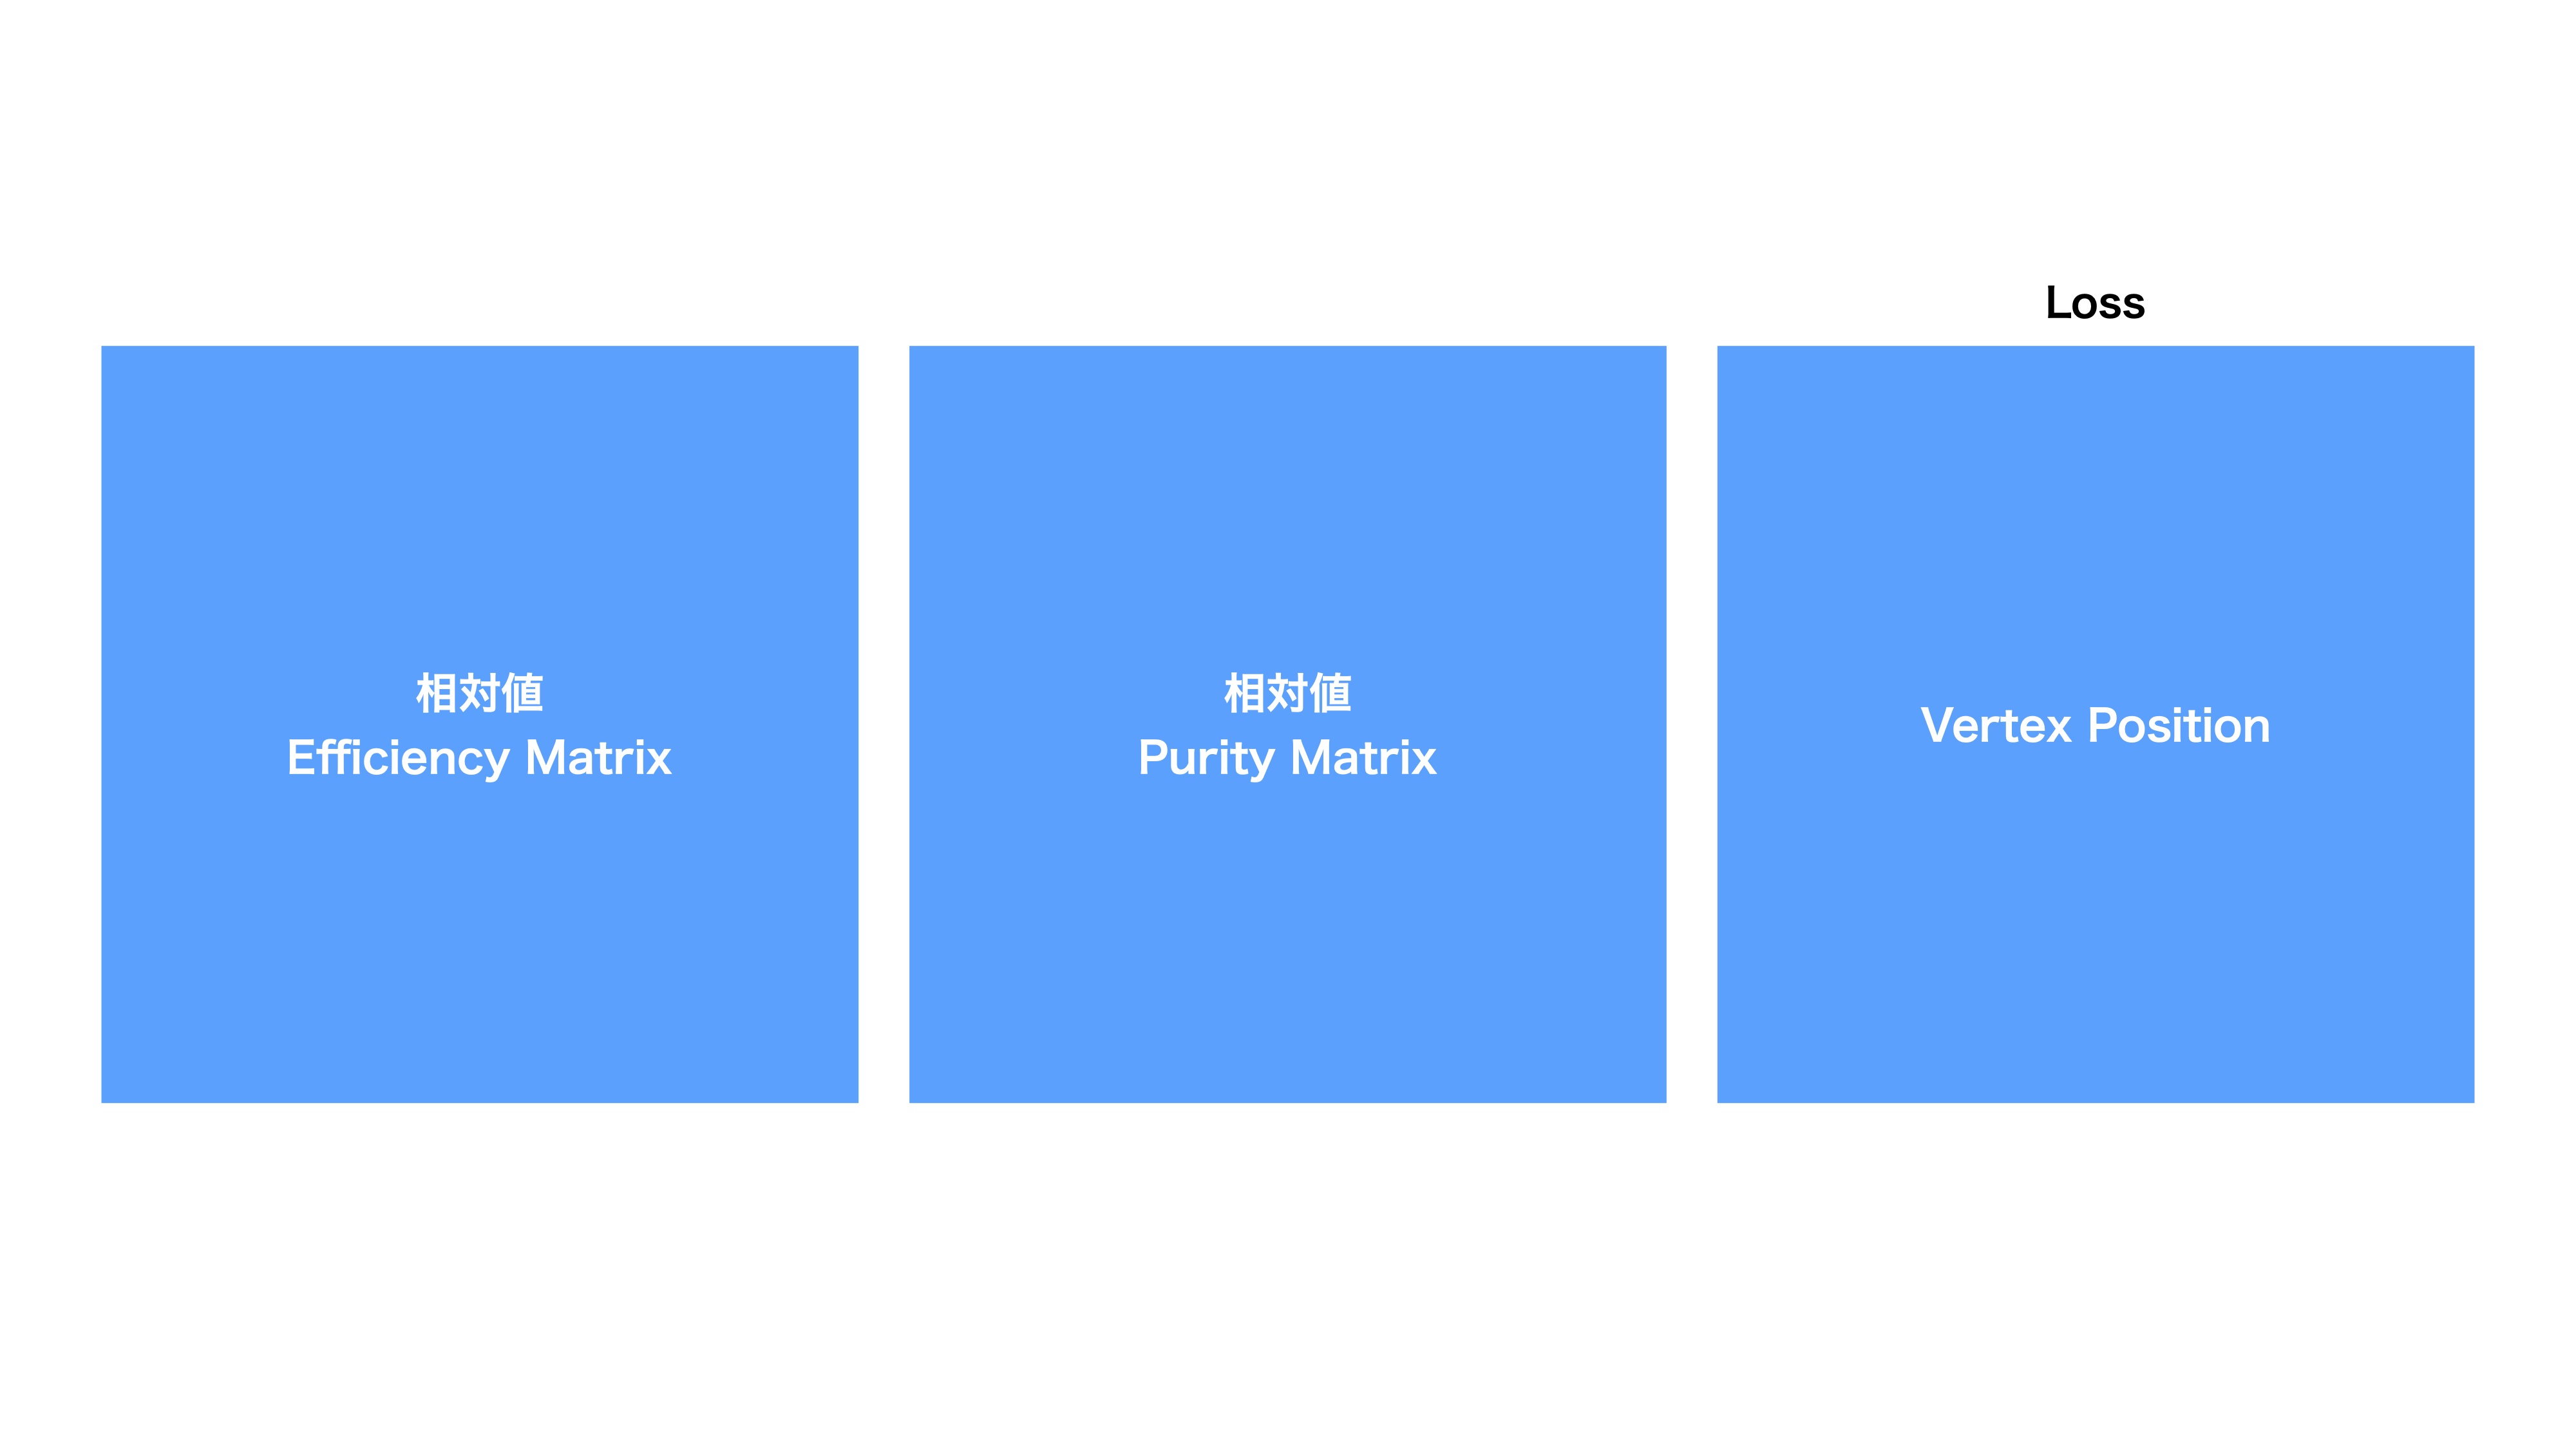
\includegraphics[trim = 0 220 0 220, width=0.9\textwidth, clip]{Figure/3Networks/3-3-3-2ConfusionMatrixD.png}
    \subcaption{モデルDの混合行列の相対値と崩壊点の位置}
    \label{3-3-3-2ConfusionMatrixD}
   \end{minipage}
  \caption{各ネットワークの混合行列と崩壊点の位置}
  \label{3-3-3-2ConfusionMatrices}
 %\end{tabular}
\end{figure}

ROCカーブ\\

\begin{figure}[htbp]
 \centering
 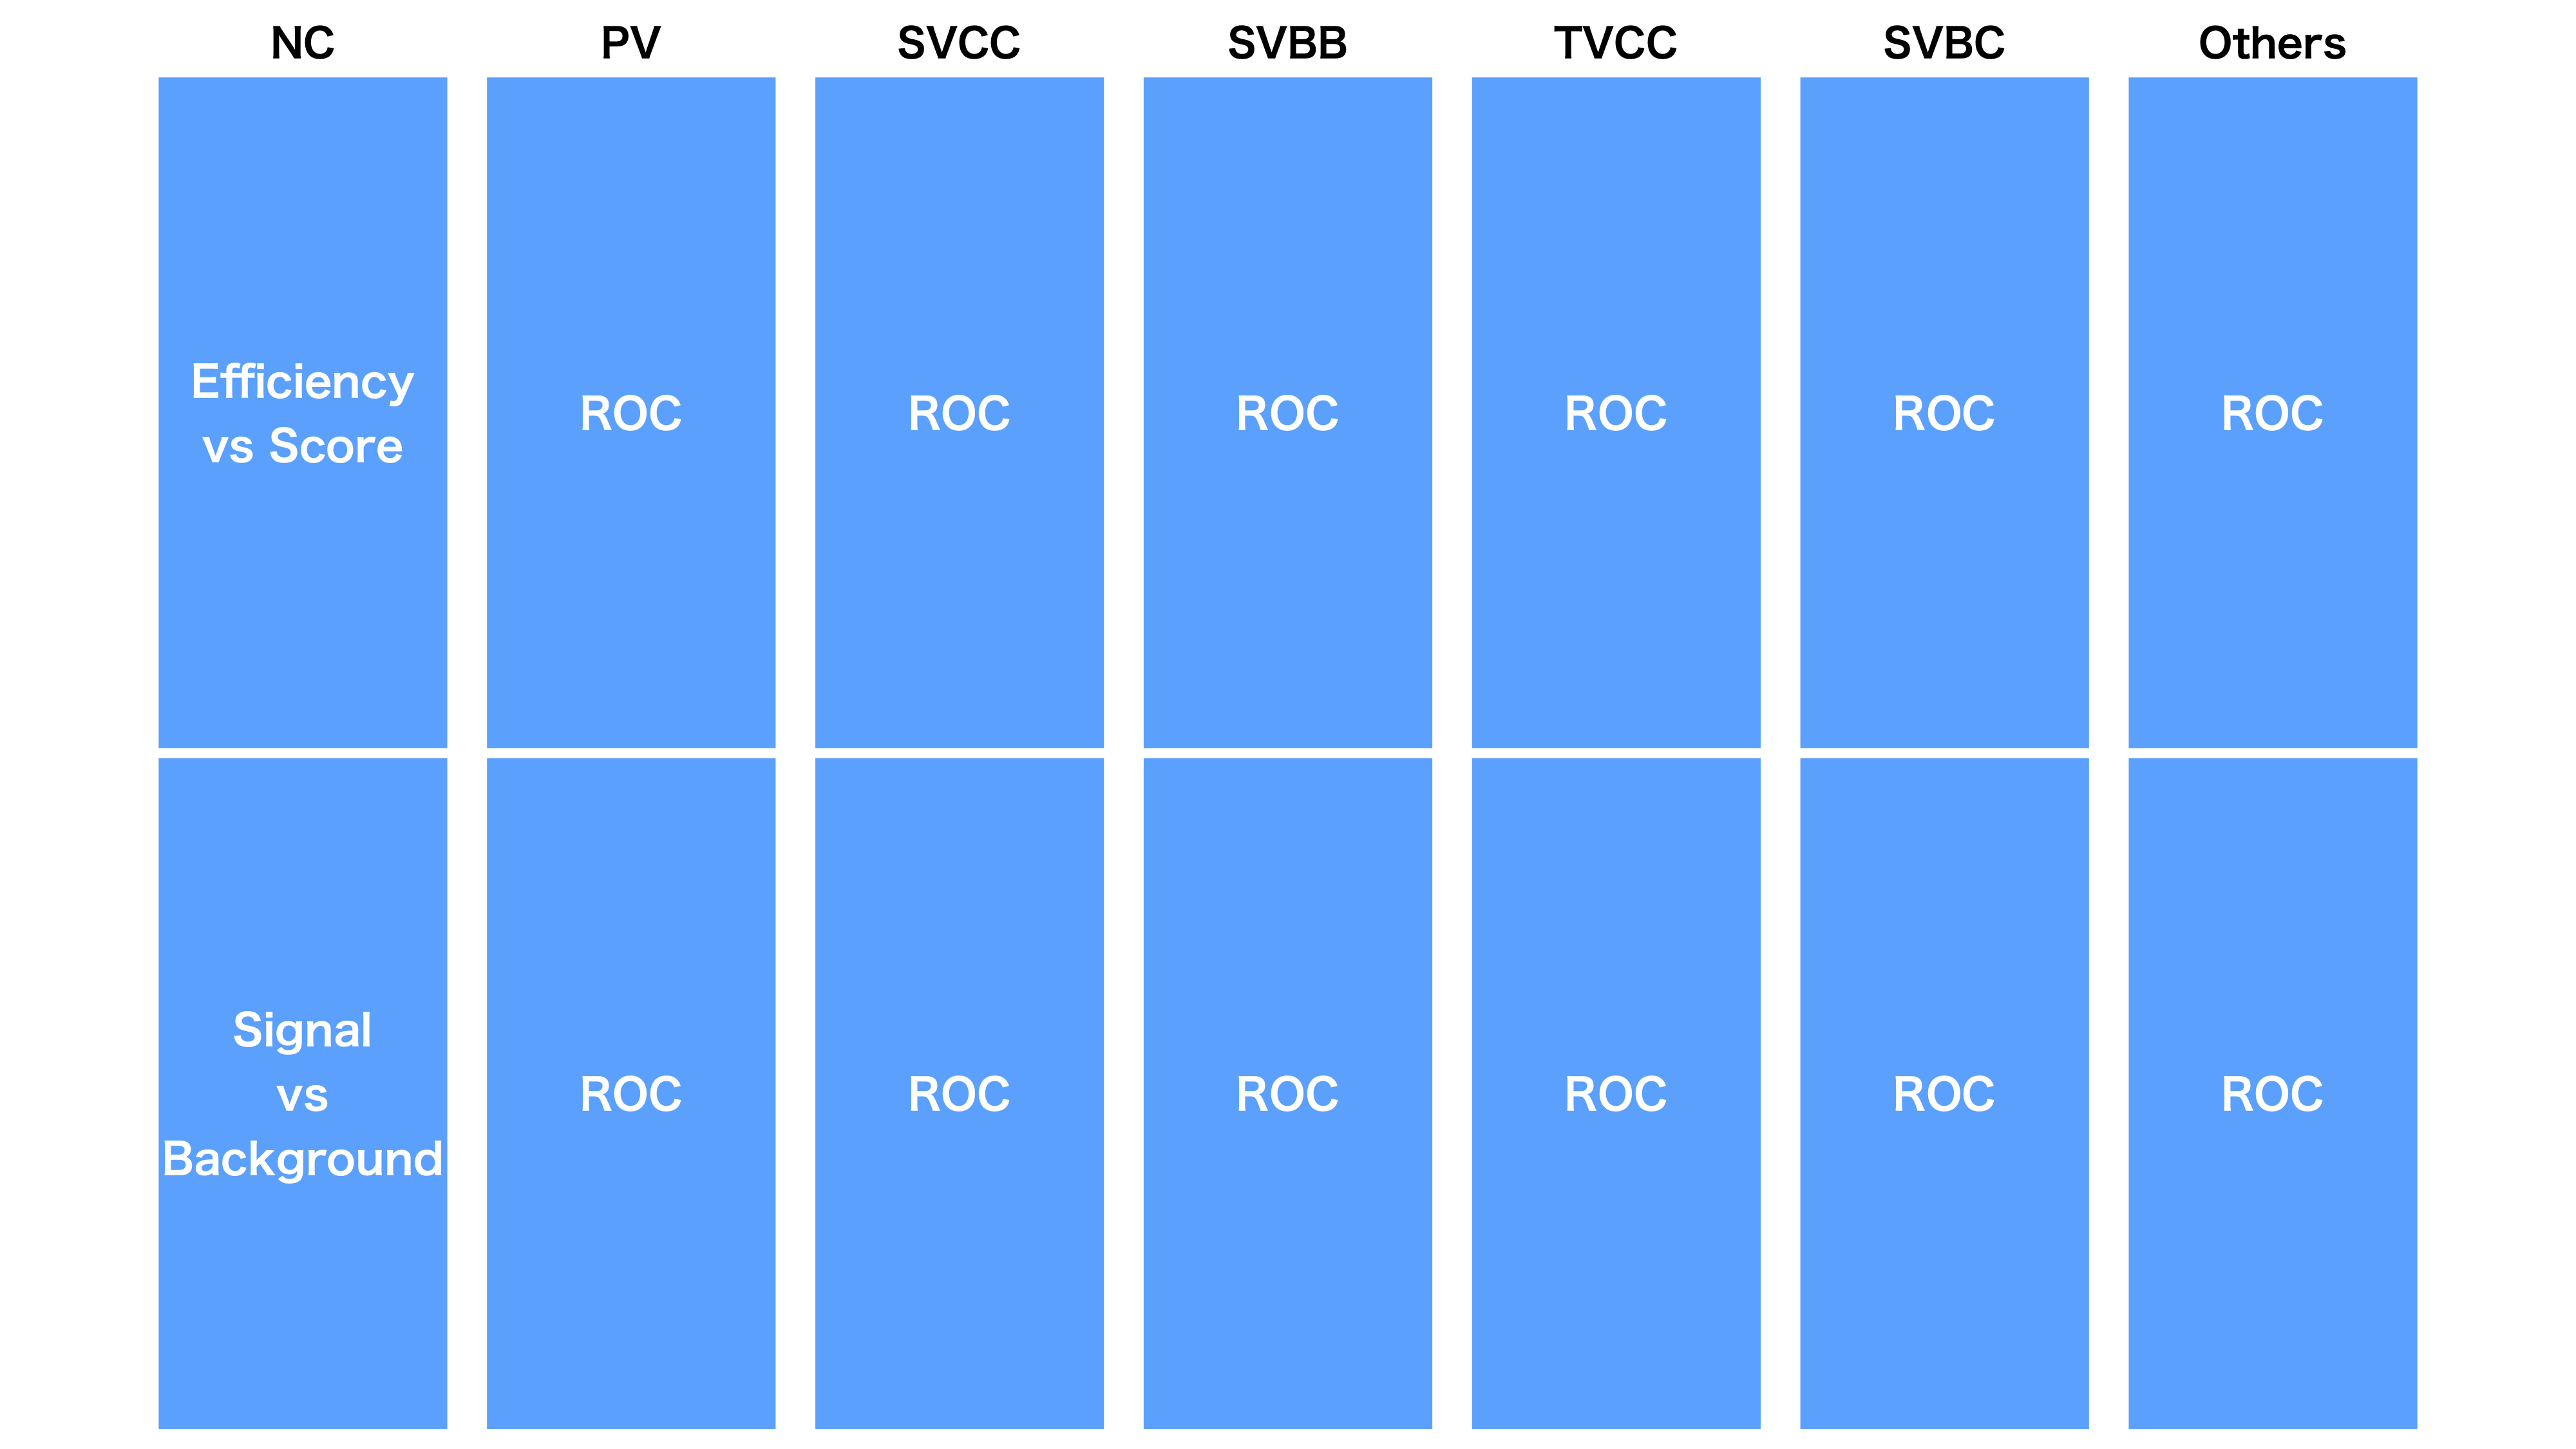
\includegraphics[width=1.0\textwidth]{Figure/3Networks/3-3-3-3ROCCurve.png}
 \caption{飛跡対についてのネットワークに関するROC曲線}
 \label{3-3-3-3ROCCurve}
\end{figure}



%%%%%%%%%%%%%%%%%%%%%%%%%%%%%%%%%%%%%%%%%%%%%%%%%%%%%%%%%%%%%%%%%%%%%%%%%%%%%%%%%%%%%%%%%%%%%%%%%%%%%
\section{任意の数の飛跡についてのネットワーク} \label{Net:VertexLSTM}

ここでは\ref{Net:forVertexFinderwithDL}節で紹介した二つのネットワークの内、任意の数の飛跡についてのネットワークに関して述べる。
前節と同様にネットワークの構造・学習・評価について\ref{Net:VLSTM:StructureofVLSTM}項・\ref{Net:VLSTM:TrainingandStrategyofVLSTM}項・\ref{Net:VLSTM:PerformanceofVLSTM}項でそれぞれ解説する。

任意の数の飛跡についてのネットワークは、崩壊点を生成するためのネットワークである。
入力は崩壊点のタネと事象中の全ての飛跡、出力は事象内のそれぞれの飛跡が飛跡対が崩壊点のタネと結合しているか否かである。

事象内の全ての飛跡を扱うに当たって、\ref{Net:Data:DataProperty}項で述べた事象中に含まれる飛跡の本数が異なっているという性質に注意せねばならない。
また二本以上の飛跡の結合を考えた際、三本、四本、五本の飛跡を取り扱えるネットワークをそれぞれ構築することはネットワークや組み合わせの数を考える上で適切ではない。
そのような不定の数の飛跡を再帰的に処理するネットワーク構造として、リカレントニューラルネットワークが考えられる。
この時、リカレントニューラルネットワークの初期状態として崩壊点のタネを用い、系列データとして事象内の全ての飛跡を入力する。
また出力の作り方はMany to Manyとし、事象内のそれぞれの飛跡が初期状態の崩壊点のタネに対して結合しているか否かを評価するネットワークを構築する。

\begin{figure}[htbp]
 \centering
 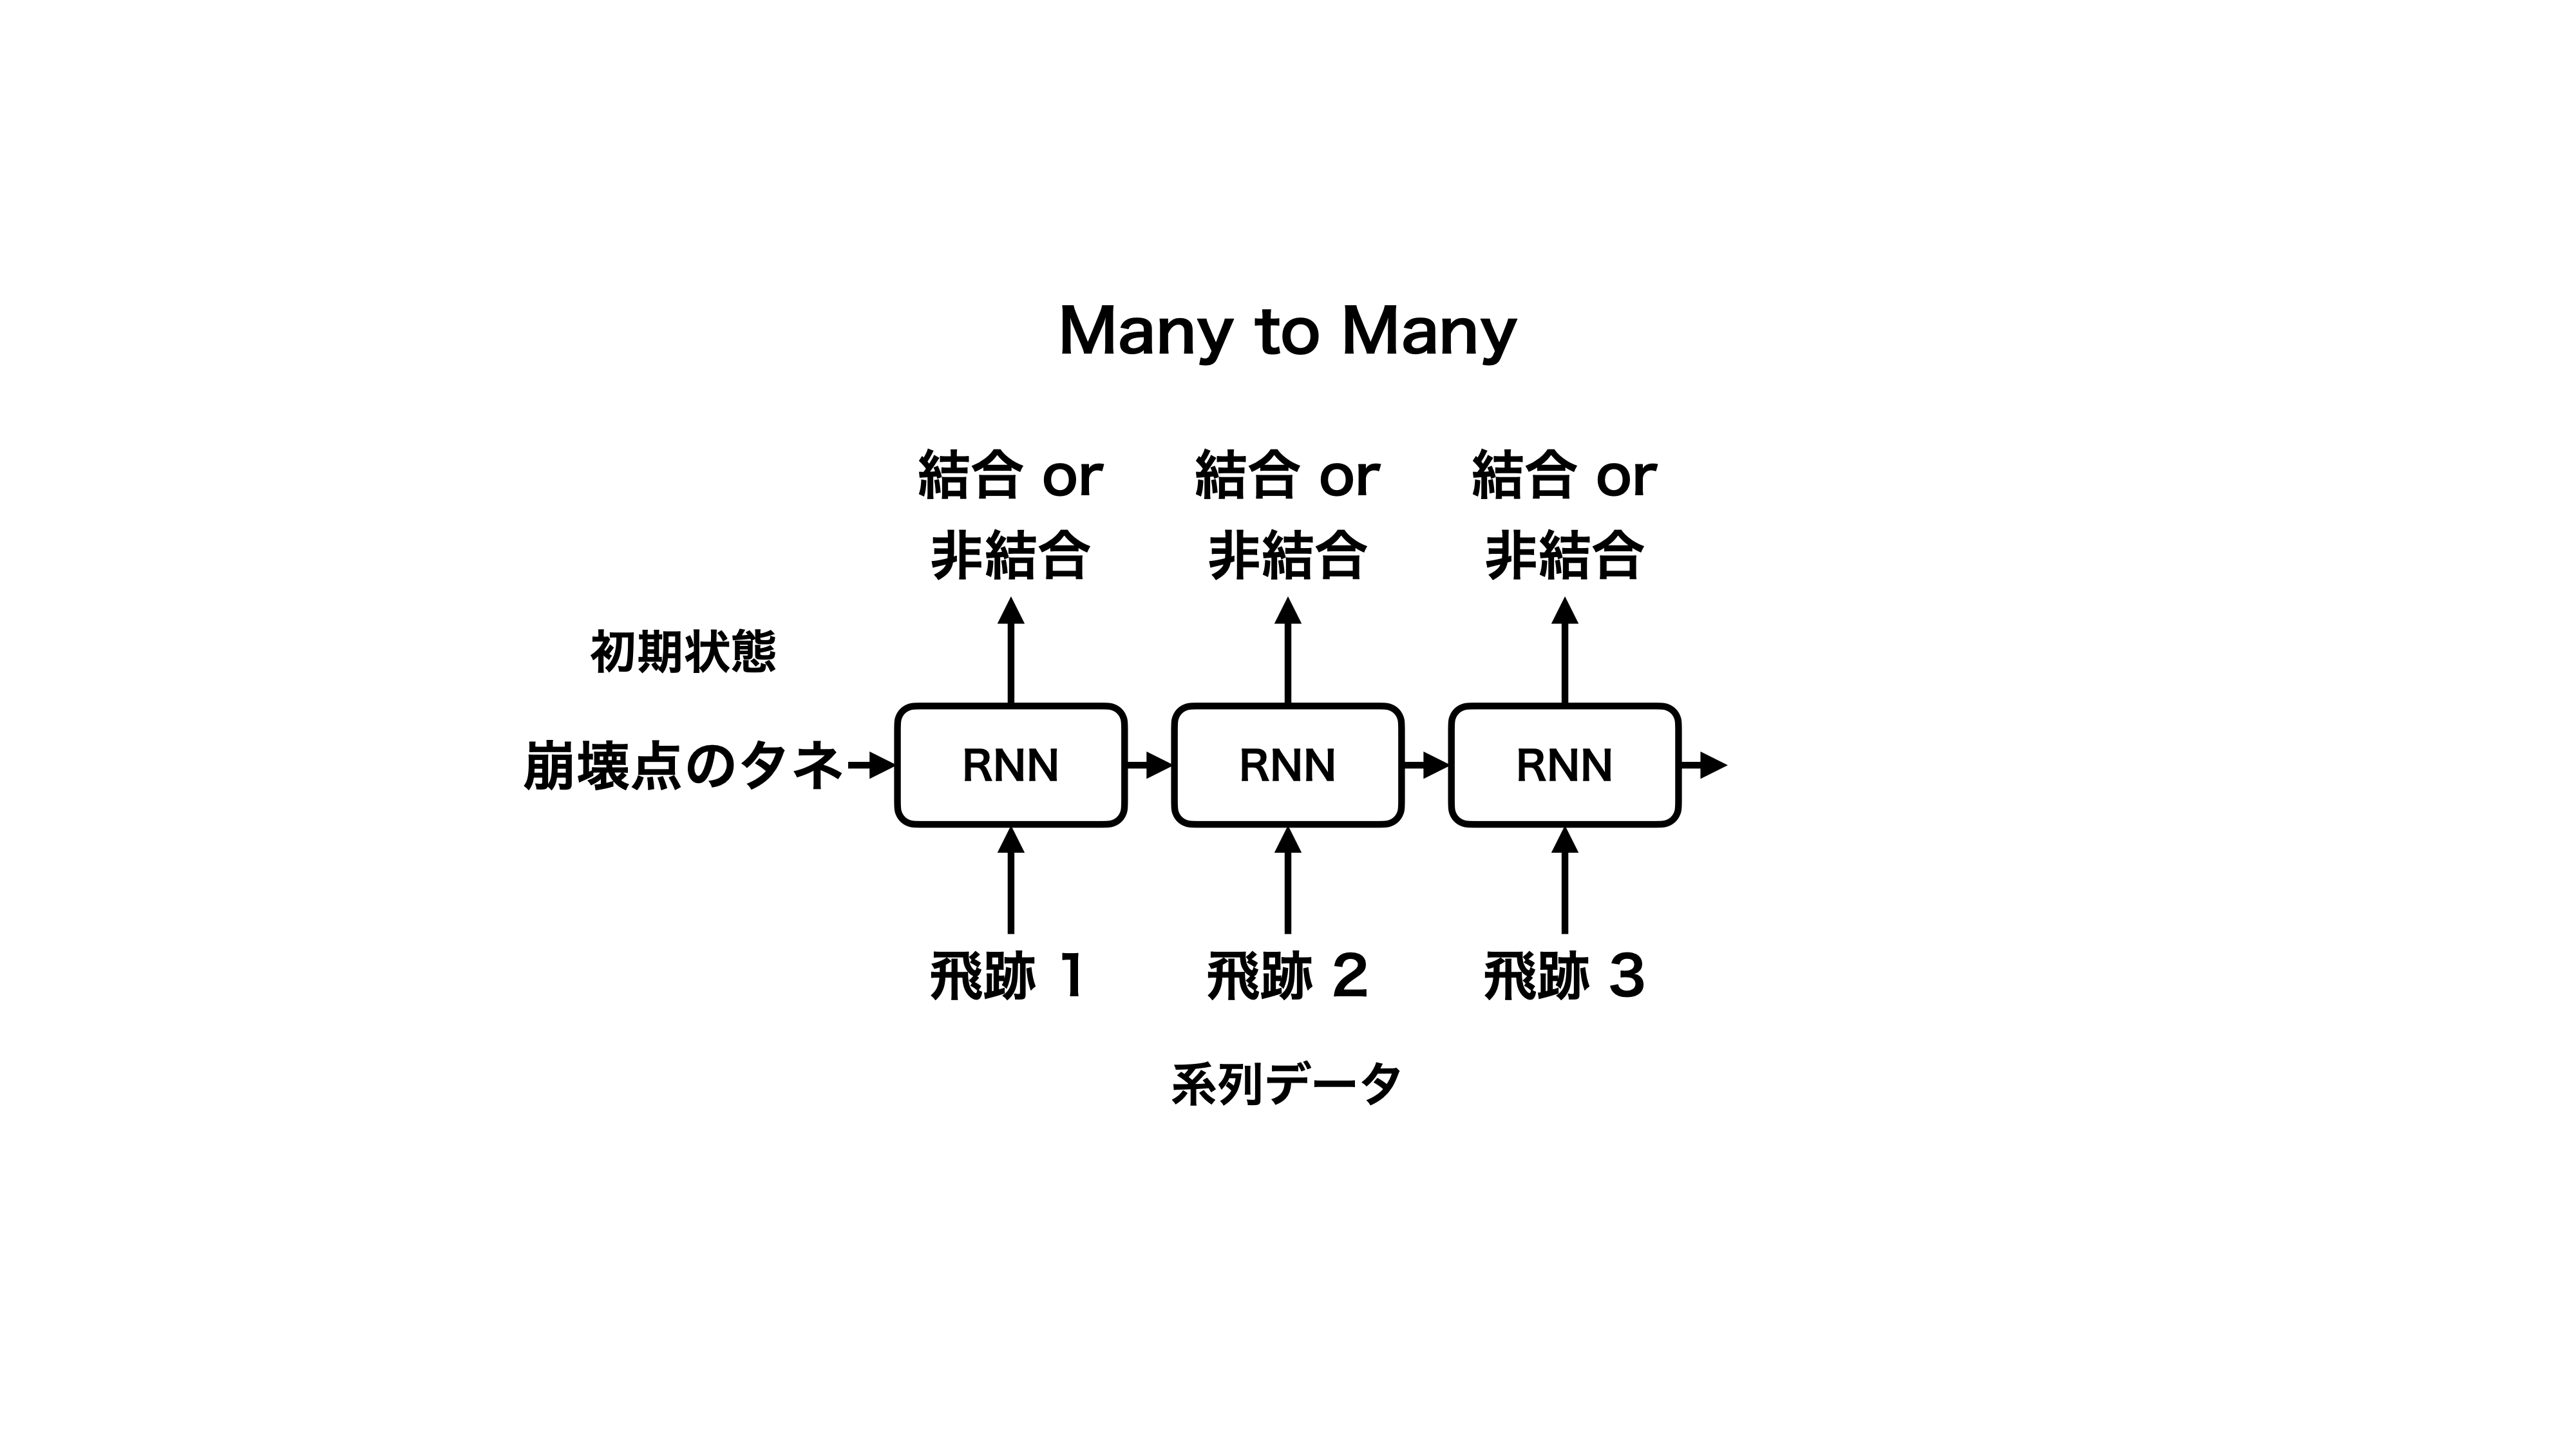
\includegraphics[trim = 200 150 200 150, width=0.9\textwidth, clip]{Figure/3Networks/3-4-0-1VertexProductionwithRNN.png}
 \caption{リカレントニューラルネットワークを用いた崩壊点生成}
 \label{3-4-0-1VertexProductionwithRNN}
\end{figure}


%%%%%%%%%%%%%%%%%%%%%%%%%%%%%%%%%%%%%%%%%%%%%%%%%%%%%%%%%%%%%%%%%%%%%%%%
\subsection{ネットワークの構造} \label{Net:VLSTM:StructureofVLSTM}

まず、任意の数の飛跡についてのネットワークとして図\ref{3-4-1-1SimpleVLSTM}のようなネットワークを考える。

\begin{figure}[htbp]
 \centering
 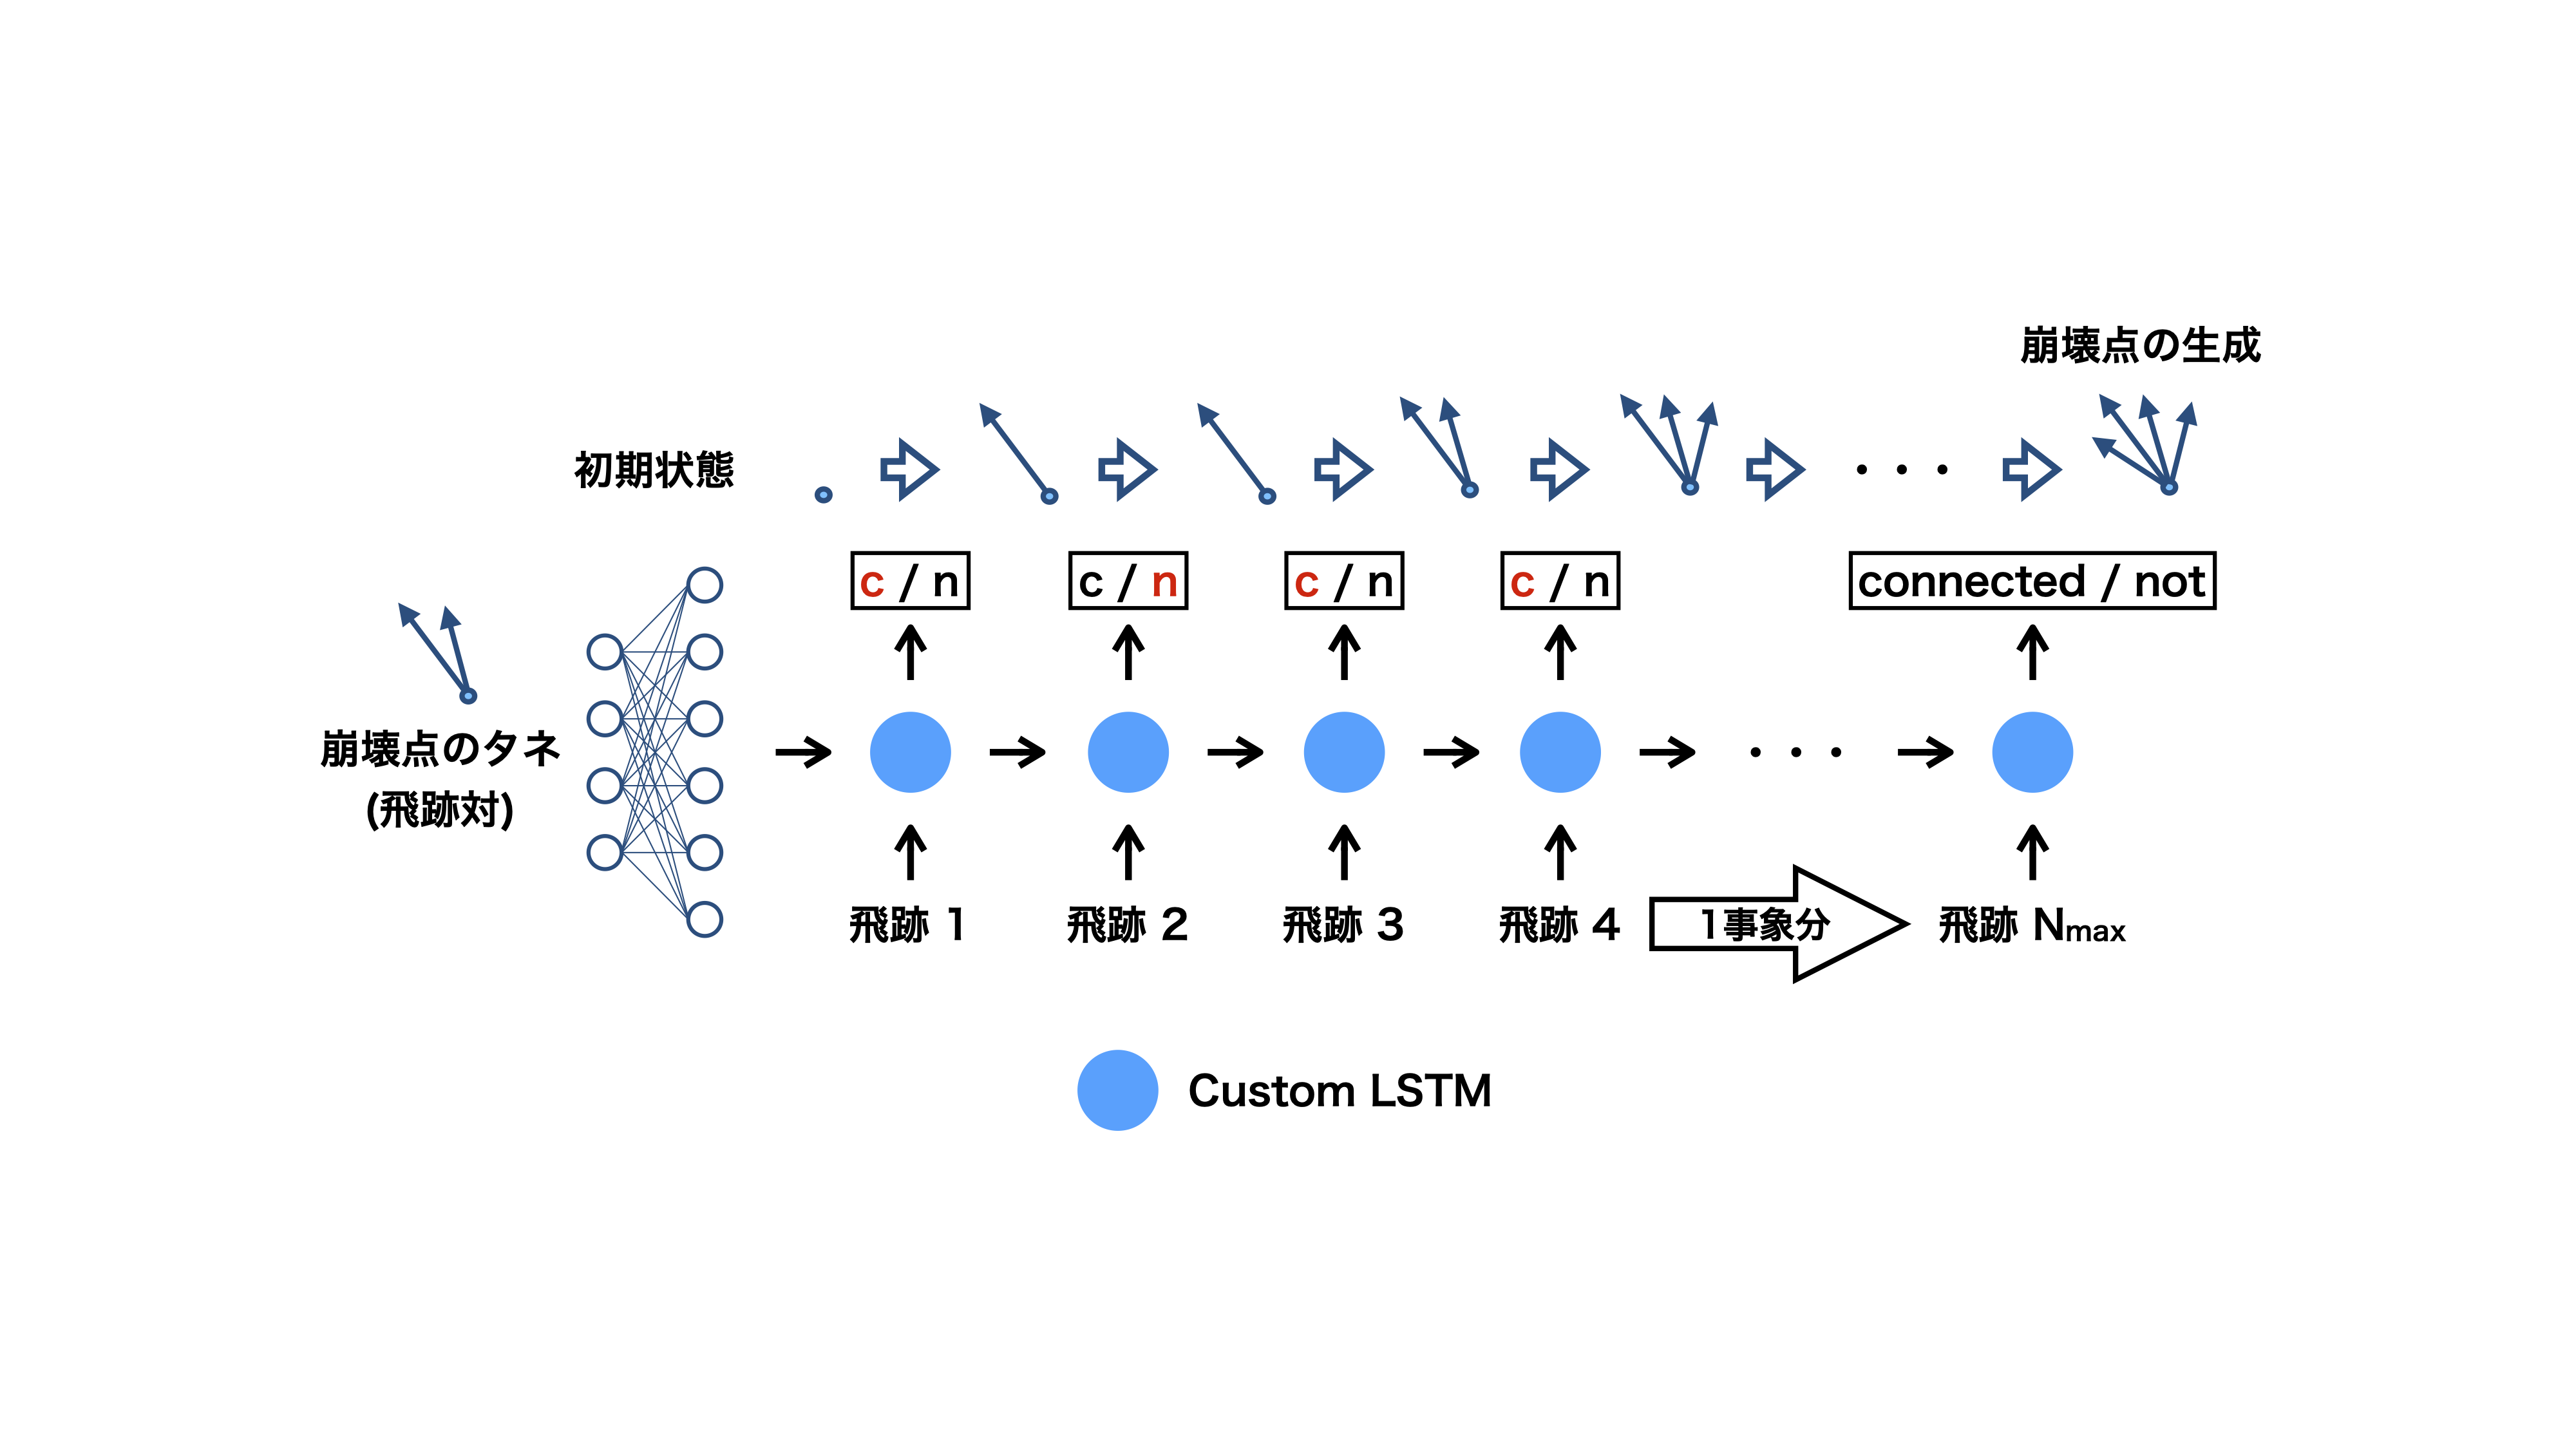
\includegraphics[trim = 100 200 100 200, width=1.0\textwidth, clip]{Figure/3Networks/3-4-1-1SimpleVLSTM.png}
 \caption{崩壊点生成のためのリカレントニューラルネットワーク構造}
 \label{3-4-1-1SimpleVLSTM}
\end{figure}

前述したように崩壊点のタネを初期状態として使用している。
実際には崩壊点のタネは飛跡対 ($44$個の変数) であり、更に全結合層を介してより抽象的な崩壊点の情報を初期状態として入力できるようにしている。
また系列データとして事象中の全ての飛跡を用いている。
出力はこの飛跡のそれぞれが崩壊点のタネと結合しているか否かである。

\ref{DL:RNN:LongShortTermMemory}で解説したようにリカレントニューラルネットワークは系列情報を保持するため直前の系列に依存するように設計されている。
しかし飛跡は本質的に順序を持っていないことに注意する必要がある。
図\ref{3-4-1-1SimpleVLSTM}では便宜的に飛跡について番号を振り表現しているが、これは人が勝手に決めた順序であり、本来事象中の飛跡は系列データではない。
したがって、リカレントニューラルネットワークをそのまま用いることはデータの性質に合わない。
この為私は、リカレントニューラルネットワークの一つであるLSTMを拡張し、新しい独自のリカレントニューラルネットワークの構造を構築した。

図\ref{3-4-1-2VLSTMStructure}はそのような独自のリカレントニューラルネットワークについての1系列分のステップの詳細である。

\begin{figure}[htbp]
 \centering
 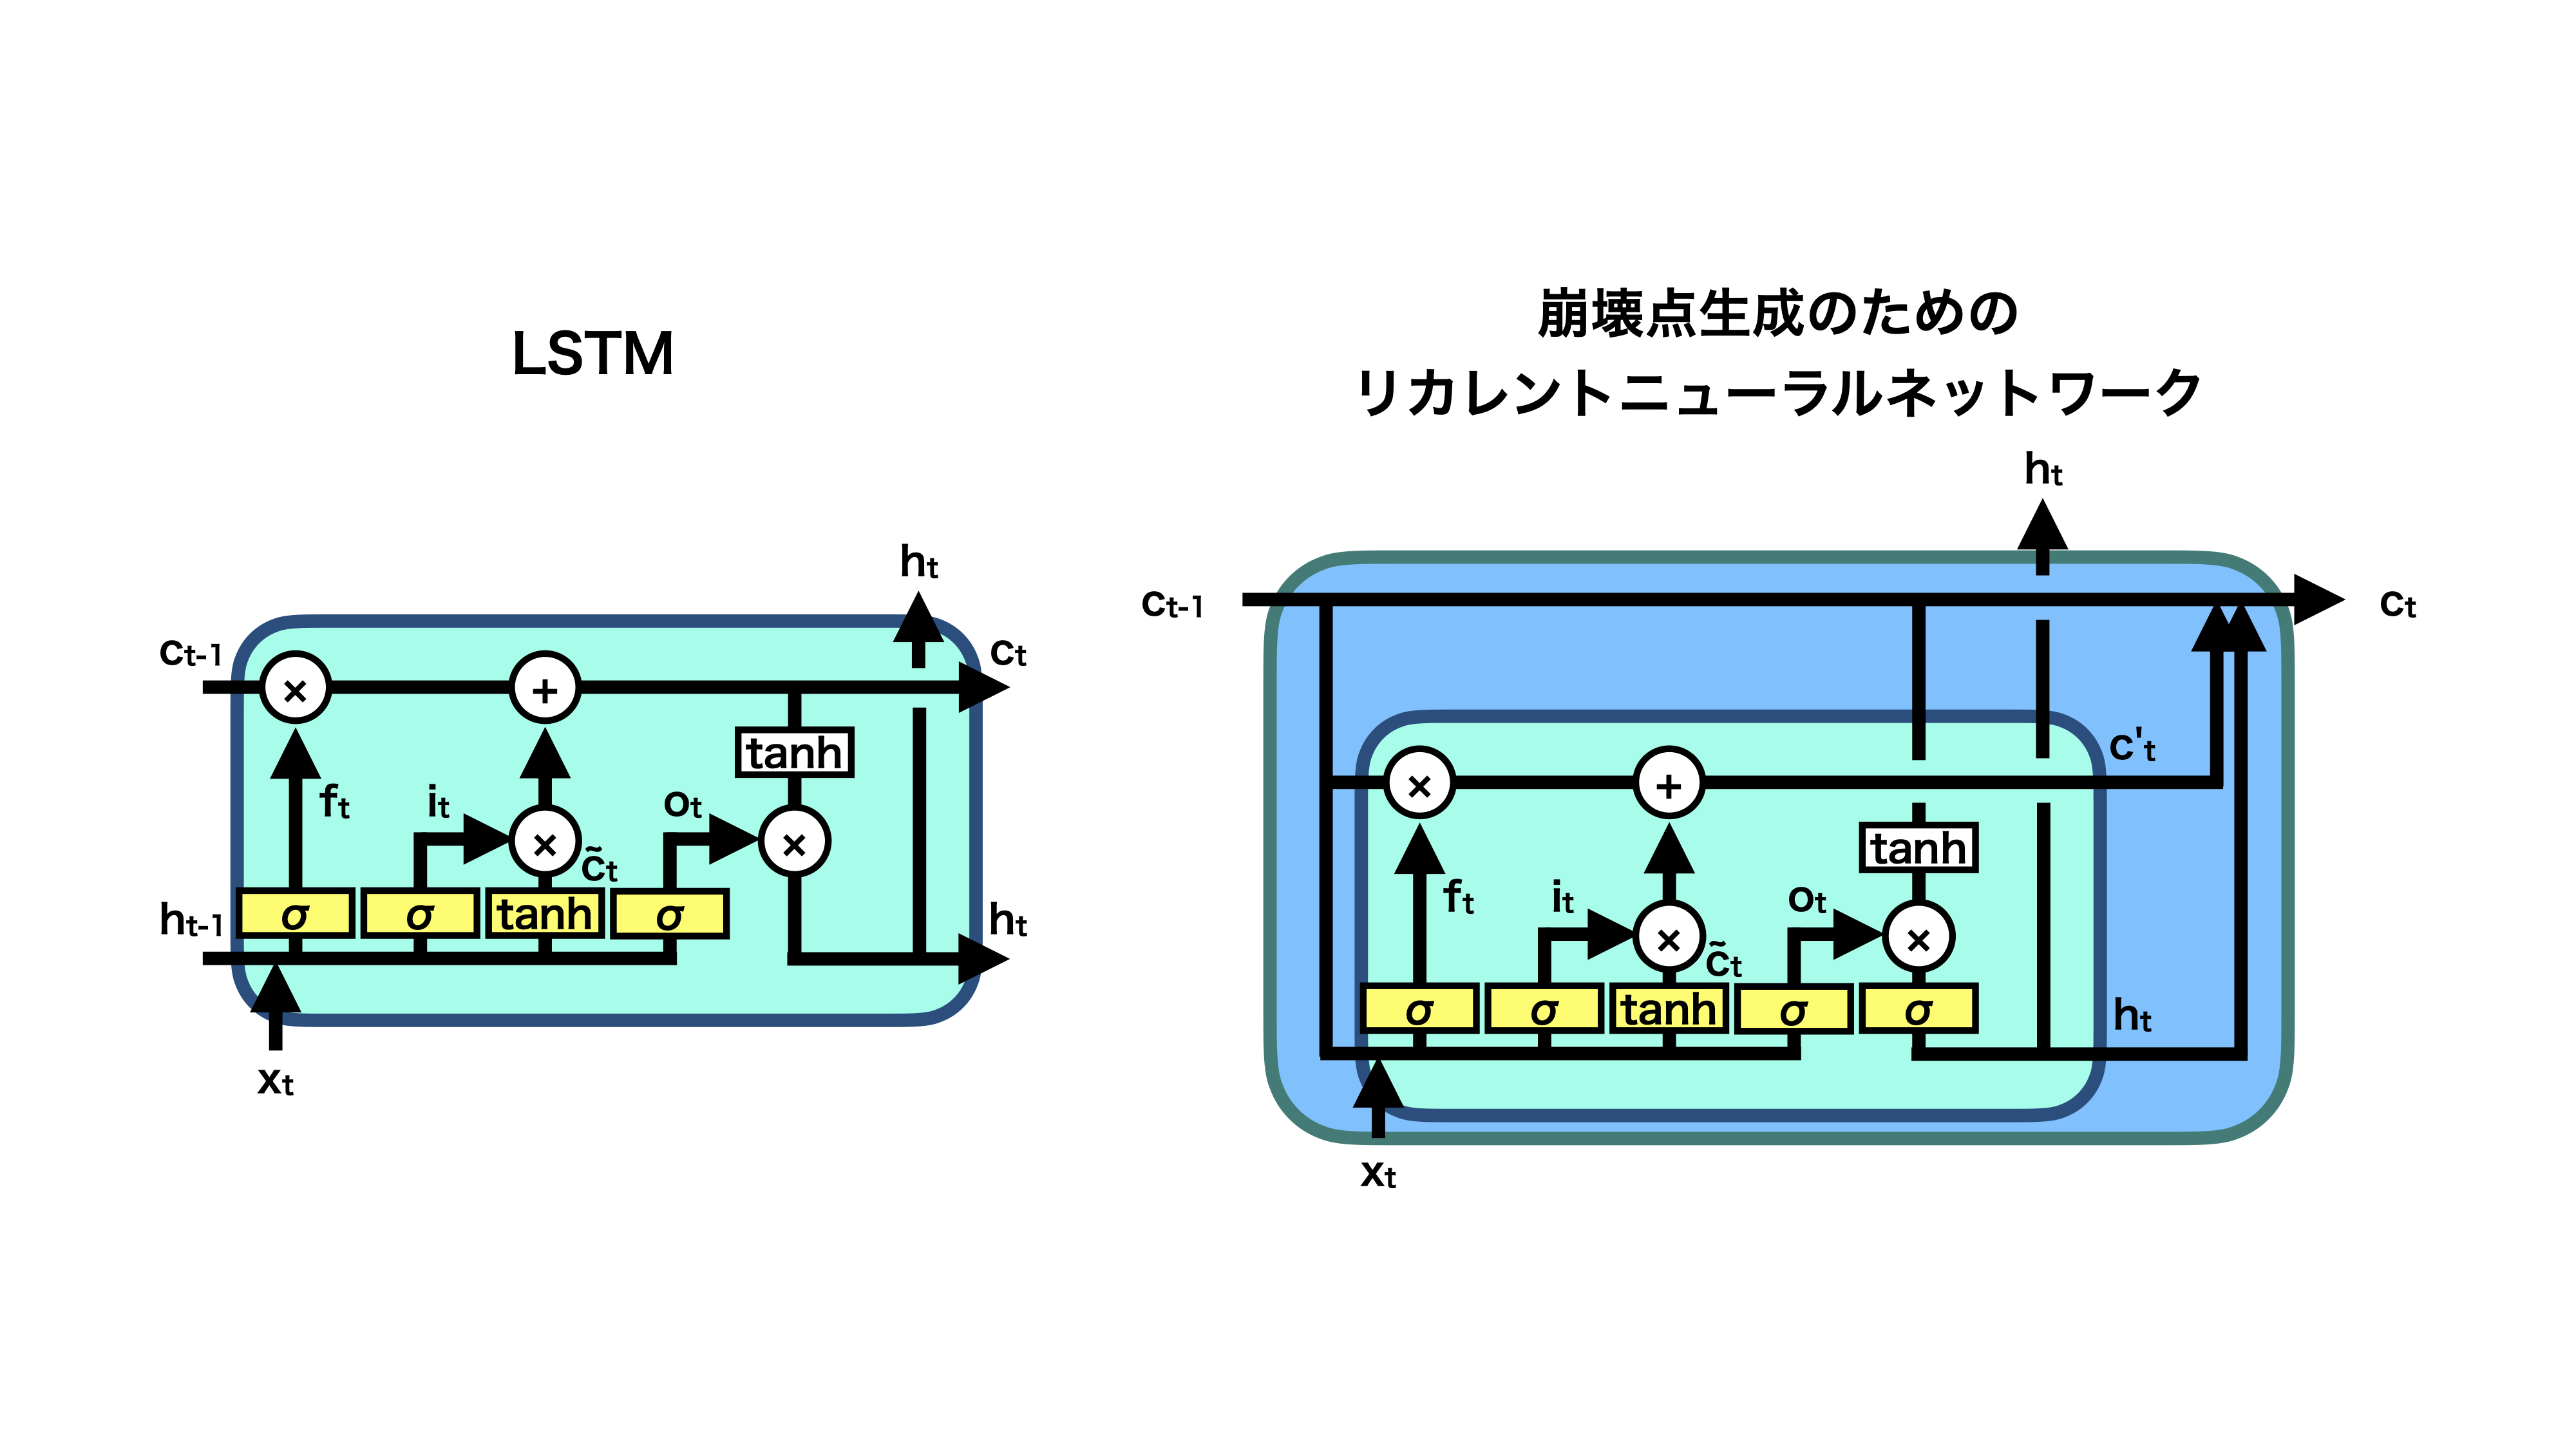
\includegraphics[trim = 0 100 0 200, width=0.9\textwidth, clip]{Figure/3Networks/3-4-1-2VLSTMStructure.png}
 \caption{系列1ステップについての独自リカレントニューラルネットワーク構造}
 \label{3-4-1-2VLSTMStructure}
\end{figure}

LSTMとの大きな構造の違いは、短期記憶である${\mbox{\boldmath{$h$}}}_t$が隠れ状態として入出力されていない点である。
入力は隠れ状態の記憶セル${\mbox{\boldmath{$c$}}}_{t-1}$と系列データ${\mbox{\boldmath{$x$}}}_t$の二つである。
また出力は結合・非結合を判定する${\mbox{\boldmath{$h$}}}_t$と隠れ状態の記憶セル${\mbox{\boldmath{$c$}}}_{t}$の二つである。
隠れ状態として${\mbox{\boldmath{$h$}}}_t$が使用されていないため、内部の構造も通常のLSTMとは少し異なり、出力${\mbox{\boldmath{$h$}}}_{t}$と記憶セル${\mbox{\boldmath{$c$}}}_{t}$はそれぞれ
\begin{equation}
 \begin{split}
  &{\mbox{\boldmath{$c$}}}_{t} 
  = (1-{\mbox{\boldmath{$h$}}}_t) {\mbox{\boldmath{$c$}}}_{t-1} + {\mbox{\boldmath{$h$}}}_t {\mbox{\boldmath{$c'$}}}_{t}\\
  &{\mbox{\boldmath{$c'$}}}_{t}
  = {\mbox{\boldmath{$c$}}}_{t-1} \  \sigma (W_f {\mbox{\boldmath{$x$}}}_t + R_f {\mbox{\boldmath{$c$}}}_{t-1}) 
  + \tanh (W_c {\mbox{\boldmath{$x$}}}_t + R_c {\mbox{\boldmath{$c$}}}_{t-1}) \  \sigma (W_i {\mbox{\boldmath{$x$}}}_t + R_i {\mbox{\boldmath{$c$}}}_{t-1})\\
  &{\mbox{\boldmath{$h$}}}_{t} 
  = \sigma (D_h [\tanh({\mbox{\boldmath{$c$}}}_{t-1}) \  \sigma (W_o {\mbox{\boldmath{$x$}}}_t + R_o {\mbox{\boldmath{$c$}}}_{t-1}) ])
 \end{split}
\end{equation}
となる。
第二式の${\mbox{\boldmath{$c'$}}}_{t}$は更新された記憶セルを示している。
第三式は出力ゲートに更に全結合層を掛けた形となっており、二値分類の為の出力を作成している。
第一式では、更新された記憶セル${\mbox{\boldmath{$c'$}}}_{t}$と直前の系列での記憶セル${\mbox{\boldmath{$c$}}}_{t-1}$、出力${\mbox{\boldmath{$h$}}}_{t}$を用いて現在の記憶セル${\mbox{\boldmath{$c$}}}_{t}$を計算している。
二値分類であるので、${\mbox{\boldmath{$h$}}}_{t}$は$0$から$1$の値を持つはずである。
したがって、第一式は結合(${\mbox{\boldmath{$h$}}}_{t} \sim 1$)していれば更新された記憶セル${\mbox{\boldmath{$c'$}}}_{t}$が、非結合(${\mbox{\boldmath{$h$}}}_{t} \sim 0$)であれば、直前の系列での記憶セル${\mbox{\boldmath{$c$}}}_{t-1}$が現在の記憶セル${\mbox{\boldmath{$c$}}}_{t}$となることを示している。

初期状態は崩壊点のタネであるので、以上の演算は次のように (図\ref{3-4-1-3Interpretation}) 解釈できる。

\begin{enumerate}
 \item $t-1$番目の崩壊点${\mbox{\boldmath{$c$}}}_{t-1}$と$t$番目の飛跡${\mbox{\boldmath{$x$}}}_{t}$が結合しているか否かの評価${\mbox{\boldmath{$h$}}}_{t}$を行う
 \item $t-1$番目の崩壊点${\mbox{\boldmath{$c$}}}_{t-1}$と$t$番目の飛跡${\mbox{\boldmath{$x$}}}_{t}$を用いて更新された崩壊点${\mbox{\boldmath{$c'$}}}_{t}$を計算する
 \item $t-1$番目の崩壊点${\mbox{\boldmath{$c$}}}_{t-1}$と$t$番目の飛跡${\mbox{\boldmath{$x$}}}_{t}$が結合しているならば更新された崩壊点${\mbox{\boldmath{$c'$}}}_{t}$を、結合していないならば$t-1$番目の崩壊点${\mbox{\boldmath{$c$}}}_{t-1}$を$t$番目の崩壊点${\mbox{\boldmath{$c$}}}_{t}$として選択する
\end{enumerate}

\begin{figure}[htbp]
 \centering
 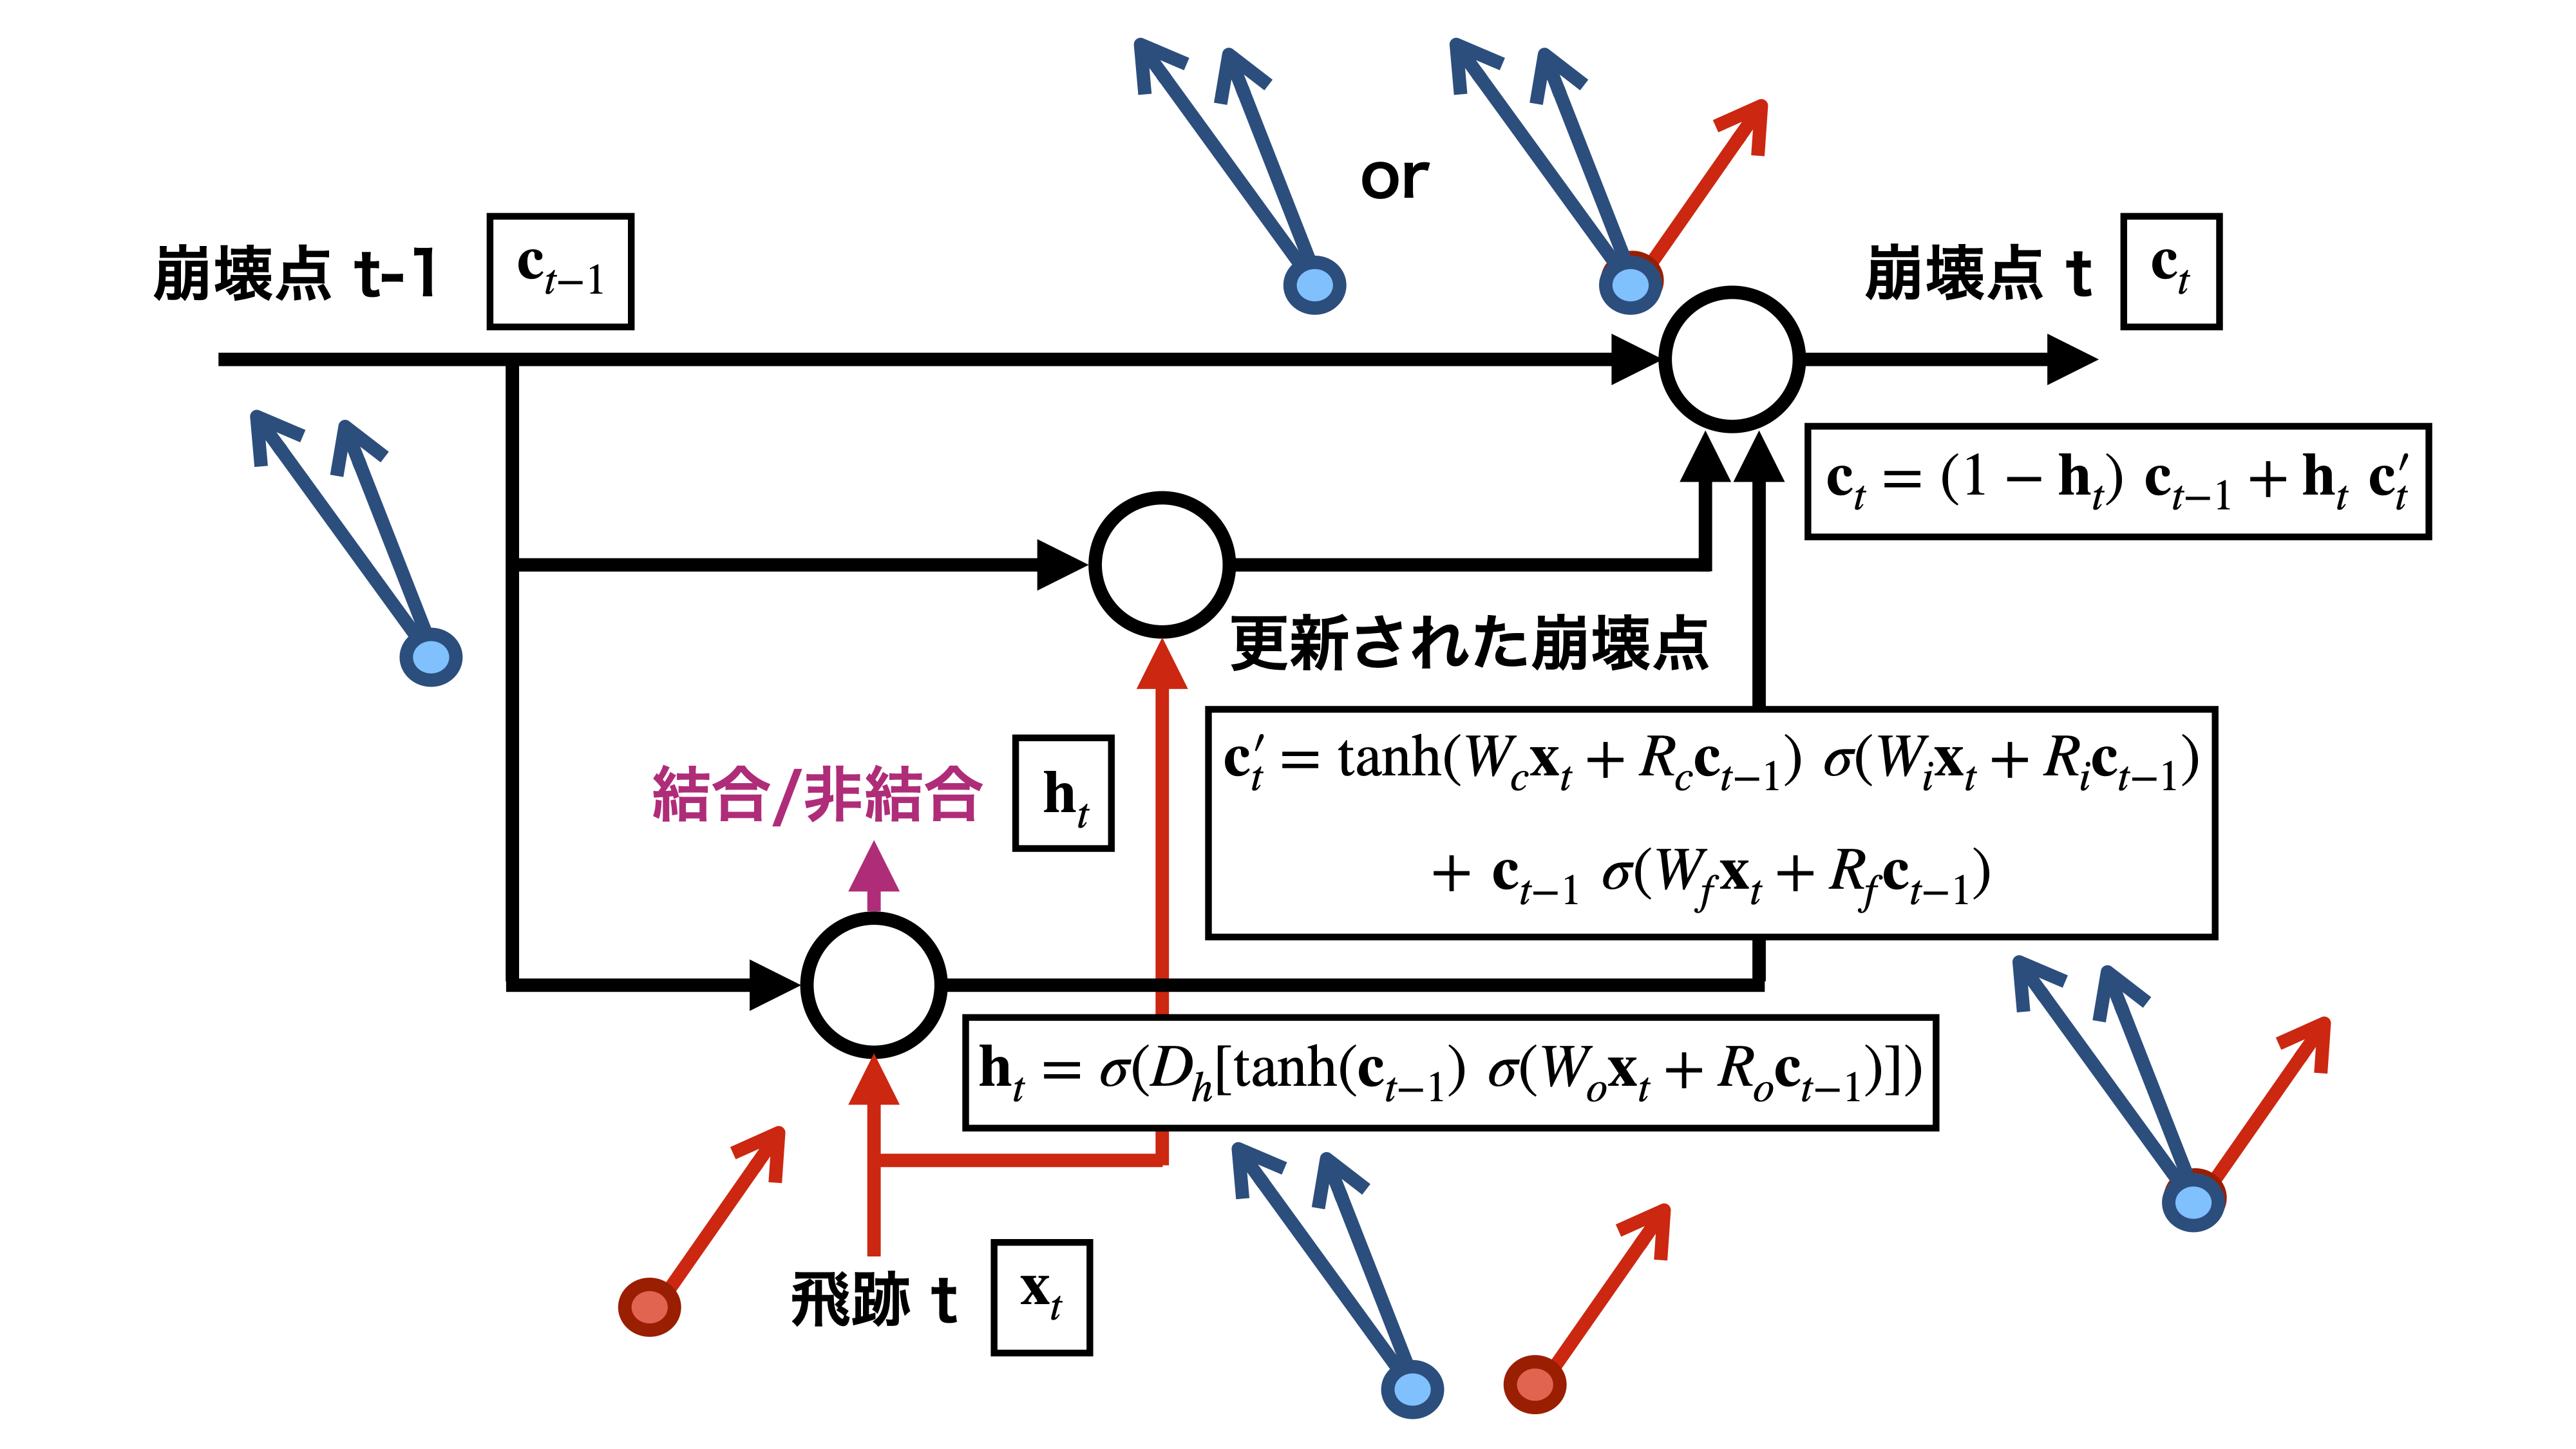
\includegraphics[width=0.9\textwidth, clip]{Figure/3Networks/3-4-1-3Interpretation.png}
 \caption{独自リカレントニューラルネットワーク構造の解釈}
 \label{3-4-1-3Interpretation}
\end{figure}

このように独自リカレントニューラルネットワークによって事象中の飛跡の順序にはできる限り依存させず、更に崩壊点のタネに対して飛跡を足していくことによって更新される崩壊点の情報を表現している。

私たちはシミュレーションデータとして既に一つの事象分の全ての飛跡についての情報を持っている。
したがって、作成したリカレントニューラルネットワークをエンコーダー・デコーダーモデルに組み込むことで、事象についての情報 (コンテキスト) を活用することができると考えられる。
また、エンコーダー・デコーダーモデルの間にAttentionを組み込むことも同様に自然な発想である。
その様なネットワークを図\ref{3-4-1-4EncoderDecoderVLSTM}に示す。

\begin{figure}[htbp]
 \centering
 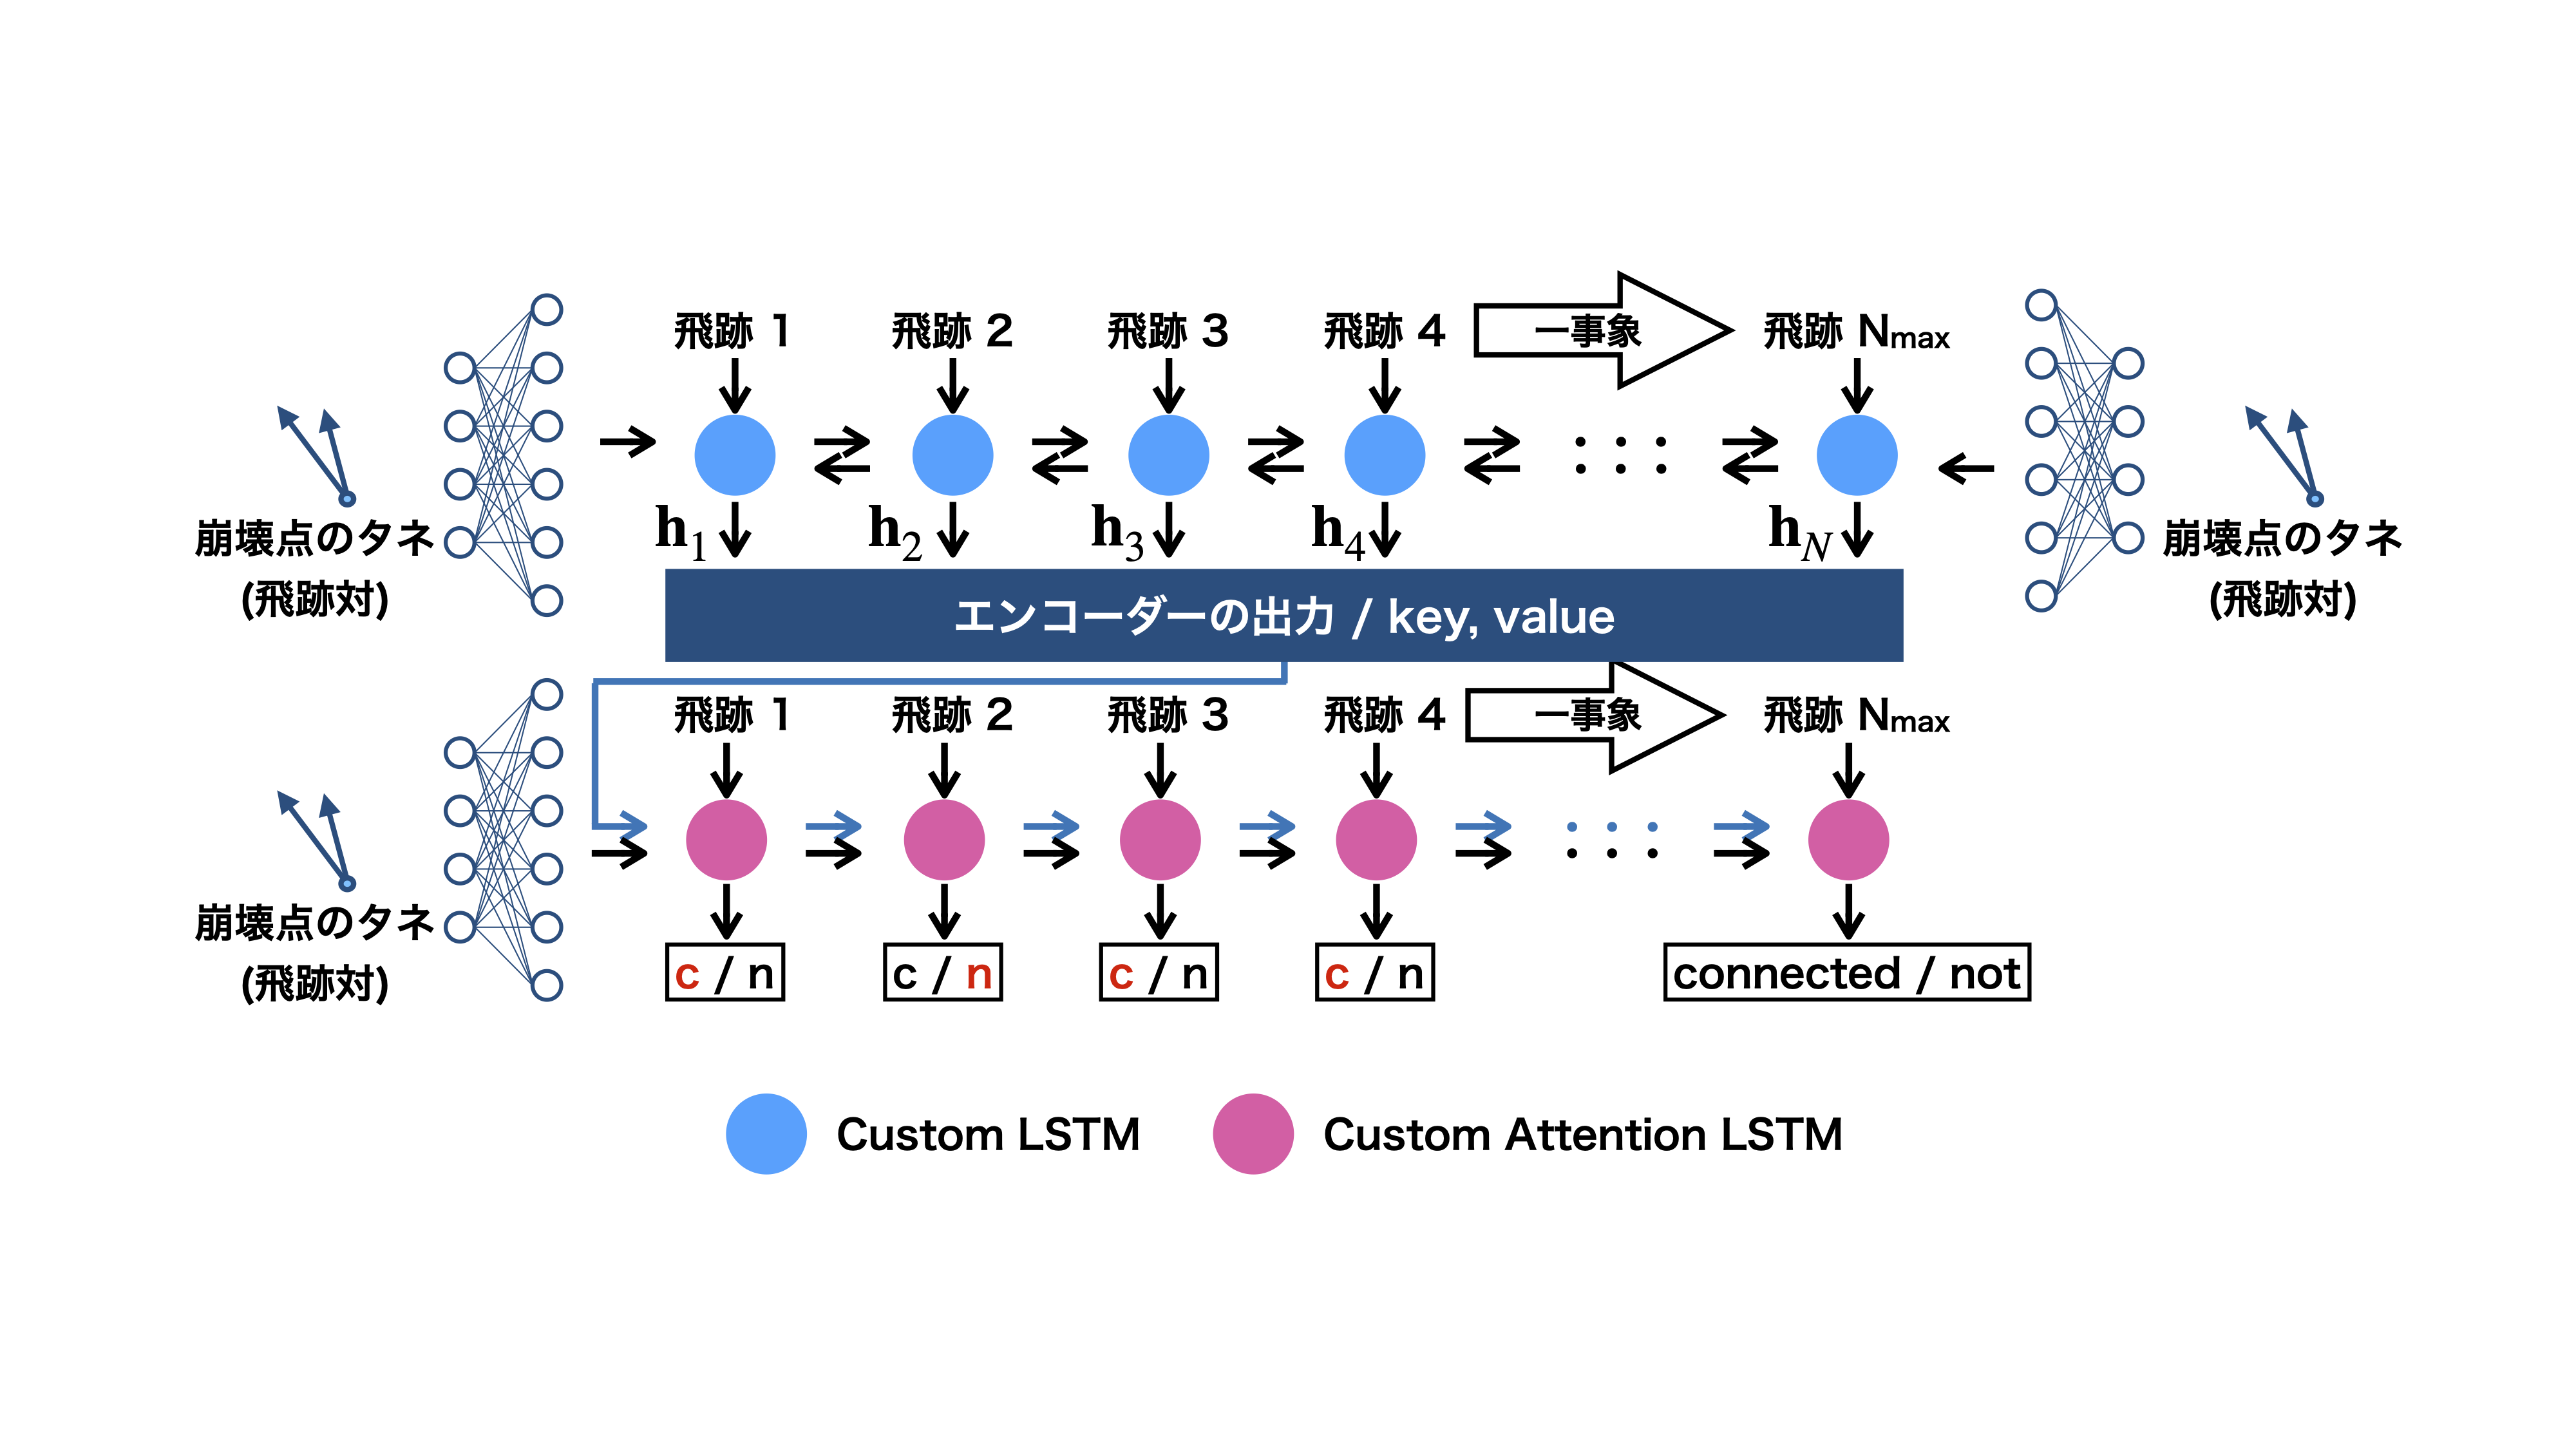
\includegraphics[trim = 100 200 100 100, width=1.0\textwidth, clip]{Figure/3Networks/3-4-1-4EncoderDecoderVLSTM.png}
 \caption{Attentionを組み込んだエンコーダー・デコーダーモデルへの拡張}
 \label{3-4-1-4EncoderDecoderVLSTM}
\end{figure}

図の上部はエンコーダー部である。
エンコーダー部では事象中の飛跡から事象全体の情報 (コンテキスト) を抽出している。
ここでは先ほどの図\ref{3-4-1-1SimpleVLSTM}で紹介したネットワークを双方向リカレントニューラルネットワークとして使用している。
ただし、出力${\mbox{\boldmath{$h$}}}_{t}$の次元を減らさないようにするため全結合層$D_h$を取り除いている。
また図中で表現しているように、双方向から入力されている崩壊点のタネはそれぞれ別の全結合層によって情報を抽象化されている。

図の下部はデコーダー部である。
デコーダー部ではエンコーダー部で抽出された情報と崩壊点のタネ、事象中の飛跡を使用して崩壊点のタネにそれぞれの飛跡が結合しているか否かを判別している。
エンコーダー部で抽出された情報はAttentionによって適切に処理され、デコーダー部の"ある"飛跡がエンコーダー部の任意の飛跡に対して注意を払って、事象中の情報を取得できるようになっている。
またエンコーダー・デコーダーモデルへの拡張後も、このネットワークの基本構造がリカレントニューラルネットワークであることに変わりはない為、デコーダー部の飛跡の本数を任意に変えることが可能である。

図\ref{3-4-1-2VLSTMStructure}で示したネットワーク構造はAttentionには対応していないため、新たなネットワークの構築が必要である。(図\ref{3-4-1-5AttentionVLSTM})

\begin{figure}[htbp]
 \centering
 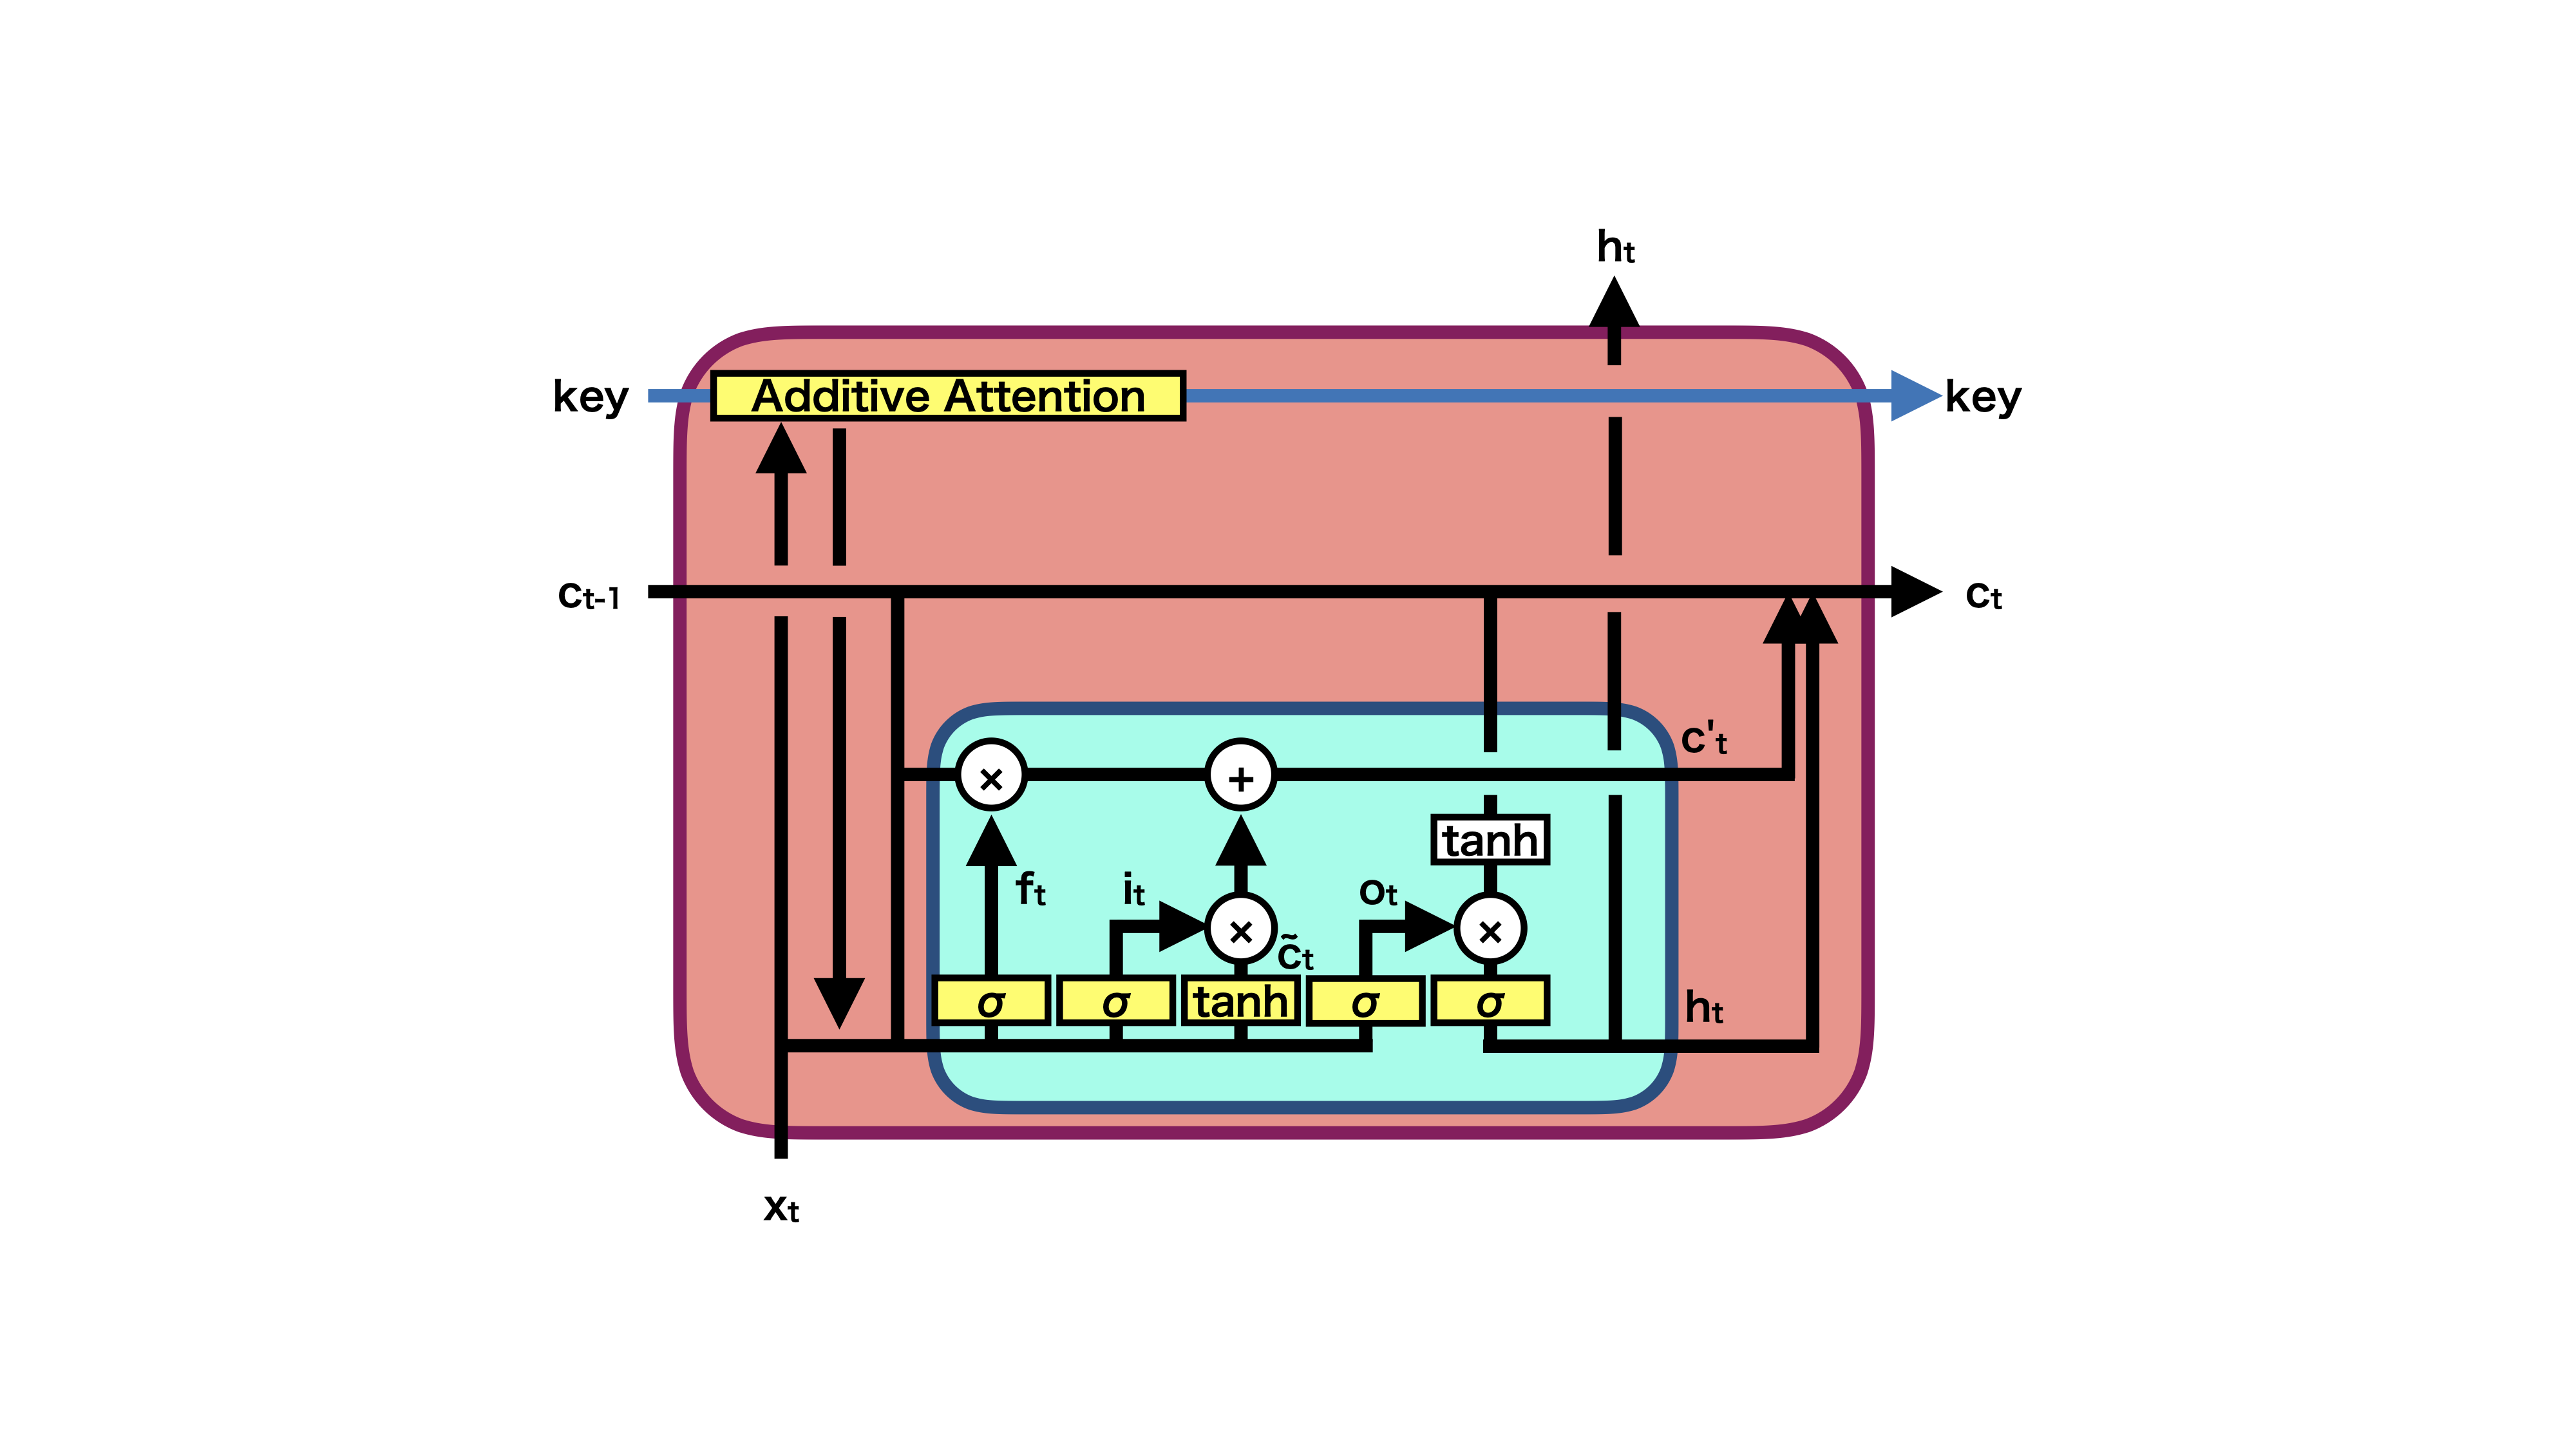
\includegraphics[trim = 100 0 100 0, width=0.9\textwidth, clip]{Figure/3Networks/3-4-1-5AttentionVLSTM.png}
 \caption{独自リカレントニューラルネットワークのAttentionへの拡張}
 \label{3-4-1-5AttentionVLSTM}
\end{figure}

本研究では、エンコーダー部で抽出された情報 (key) はリカレントニューラルネットワークの隠れ状態の一つとして入力している。
また、このkeyはネットワークの各ステップについて共通の値を使用しており、長期記憶・短期記憶と比べて不変記憶のような役割を果たしている。
Attention weightの計算方法としてAdditive Attentionを選択した。
$t$番目のコンテキスト${\mbox{\boldmath{$\gamma$}}}_{t}$は次のように計算される。
\begin{equation}
 \begin{split}
  {\mbox{\boldmath{$\gamma$}}}_{t} 
  &= {\mbox{\boldmath{$\alpha$}}}_{t} V\\
  {\mbox{\boldmath{$\alpha$}}}_{t}
  &= (\alpha_{t,0},\ \alpha_{t,1},\ \alpha_{t,2},\ \cdots \alpha_{t,i},\ \cdots) \\
  &= \left(\frac{\exp{({{e}}_{t,0})}}{\sum_j \exp{({{e}}_{t,j})}},\ \frac{\exp{({{e}}_{t,1})}}{\sum_j \exp{({{e}}_{t,j})}},\ \frac{\exp{({{e}}_{t,2})}}{\sum_j \exp{({{e}}_{t,j})}},\  \cdots \frac{\exp{({{e}}_{t,i})}}{\sum_j \exp{({{e}}_{t,j})}},\ \cdots\right)\\
  {\mbox{\boldmath{$e$}}}_{t}
  &={\mbox{\boldmath{$u$}}}_{\rm energy} (K\ U_{\rm key} + X_t\ U_{\rm query}) \\
 \end{split}
\end{equation}
ここで、keyを$K$、valueを$V$、$t$番目のqueryである飛跡${\mbox{\boldmath{$x$}}}_{t}$を重ねた行列を$X_t$、$t$番目のAttention weightを${\mbox{\boldmath{$\alpha$}}}_{t}$、$t$番目のqueryについてのエネルギーを${\mbox{\boldmath{$e$}}}_{t}$とした。
また、Additive Attentionにおける重み行列をそれぞれ${\mbox{\boldmath{$u$}}}_{\rm energy},\  U_{\rm key},\ U_{\rm query}$と置いた。

添字$i,\ j$はエンコーダー部の系列、添字$t$はデコーダー部の系列である。
したがって$t$番目のAttention weight${\mbox{\boldmath{$\alpha$}}}_{t}$はエンコーダー部の飛跡の数だけ要素を持っており、デコーダー部の全ての飛跡についてAttention weightを計算した時、Attention weightはエンコーダー部の飛跡の数$\times$デ
コーダー部の飛跡の数の行列となる。
このAttention weight行列はネットワーク内部を把握する上で非常に重要な情報である。
図\ref{3-4-1-5AttentionVLSTM}では表現していないがオプションとしてAttention weightを出力することで、そのようなネットワーク内部をある程度理解することができる。

得られた$t$番目のコンテキスト${\mbox{\boldmath{$\gamma$}}}_{t}$は、出力${\mbox{\boldmath{$h$}}}_{t}$や更新された崩壊点${\mbox{\boldmath{$c'$}}}_{t}$の計算に使用される。
\begin{equation}
 \begin{split}
  &{\mbox{\boldmath{$c$}}}_{t} 
  = (1-{\mbox{\boldmath{$h$}}}_t) {\mbox{\boldmath{$c$}}}_{t-1} + {\mbox{\boldmath{$h$}}}_t {\mbox{\boldmath{$c'$}}}_{t}\\
  &{\mbox{\boldmath{$c'$}}}_{t}
  = {\mbox{\boldmath{$c$}}}_{t-1} \  \sigma (W_f {\mbox{\boldmath{$x$}}}_t + R_f {\mbox{\boldmath{$c$}}}_{t-1} + C_f {\mbox{\boldmath{$\gamma$}}}_{t})\\
  &+ \tanh (W_c {\mbox{\boldmath{$x$}}}_t + R_c {\mbox{\boldmath{$c$}}}_{t-1} + C_c {\mbox{\boldmath{$\gamma$}}}_{t}) \  \sigma (W_i {\mbox{\boldmath{$x$}}}_t + R_i {\mbox{\boldmath{$c$}}}_{t-1} + C_i {\mbox{\boldmath{$\gamma$}}}_{t})\\
  &{\mbox{\boldmath{$h$}}}_{t} 
  = \sigma (D_h [\tanh({\mbox{\boldmath{$c$}}}_{t-1}) \  \sigma (W_o {\mbox{\boldmath{$x$}}}_t + R_o {\mbox{\boldmath{$c$}}}_{t-1} + C_o {\mbox{\boldmath{$\gamma$}}}_{t}) ])
 \end{split}
\end{equation}
式中ではコンテキスト${\mbox{\boldmath{$\gamma$}}}_{t}$に関する各ゲートそれぞれの重み行列を$C_f,\ C_c,\ C_i,\ C_o$と置いた。
$t$番目のコンテキスト${\mbox{\boldmath{$\gamma$}}}_{t}$についての演算を加えている点以外は図\ref{3-4-1-2VLSTMStructure}でのネットワークの演算と全く同様である。


%%%%%%%%%%%%%%%%%%%%%%%%%%%%%%%%%%%%%%%%%%%%%%%%%%%%%%%%%%%%%%%%%%%%%%%%
\subsection{ネットワークの学習と戦略} \label{Net:VLSTM:TrainingandStrategyofVLSTM}

訓練データは、初期状態としての飛跡対 (崩壊点のタネ) と事象中の全ての飛跡である。
また、正解ラベルはそれぞれの飛跡が崩壊点のタネと結合しているか否かのMC情報である。
推論時は、初期状態の崩壊点のタネとして非結合な飛跡対が入力される場合が考えられるが、本研究ではネットワークの学習時は崩壊点のタネとして結合している飛跡対 (PV・SVCC・SVBB・TVCC) のみを使用する。
ここで、準崩壊点SVBCは崩壊点生成において雑音となりうる可能性があるため含んでいない。
また、評価での特別な場合を除いて、Primary Vertexとその他のSecondary Verticesは区別していない。
これは崩壊点のタネとそれぞれの飛跡との関係においてPrimary Vertexとそれ以外の崩壊点との間に本質的な差異はないと判断した為である。

リカレントニューラルネットワークでは、推論時は系列長を変えることができるが、学習時は重み更新の計算のため系列長を揃える必要がある。\footnote{実際にはバッチサイズ毎に}
ここでの系列長は事象中の飛跡の本数であった。
このため、不足している飛跡の本数をゼロ埋め (Zero padding) し、ゼロ埋めした飛跡が学習に影響しないよう損失関数においてゼロ埋めした飛跡をマスクしている。
本研究では最も飛跡の数の多い事象との兼ね合いから系列長を$60$とし、それ以下の飛跡の本数の事象については$60$本になるように調整している。

最終的な入力変数の大きさを表\ref{VLSTMInputParameterShape}に示す。

\begin{table}[htb]
 \centering
 \small
  \begin{tabular}{c c}\hline
    崩壊点のタネ & $(samples,\ 44)$ \\
    事象中の全ての飛跡 & $(samples,\ 60,\ 23)$ \\\hline
  \end{tabular}
  \caption{任意の数の飛跡についてのネットワークの入力変数の大きさ}
  \label{VLSTMInputParameterShape}
\end{table}

ここで、第一引数はデータのサンプル数である。
訓練データは全ての崩壊点のタネについて一つのサンプルが生成されるため、全ての事象 ($\rm c\bar{c}-05,\ 06,\ \rm b\bar{b}-06,\ 07$) を使用すると非常に時間がかかる。
よって、本研究では全ての事象を使用して訓練データを作成した後、1エポック毎にランダムに$50000$サンプルを訓練に$10000$サンプルを検証に使用している。
事象中の全ての飛跡については飛跡の本数である$60$本とそれぞれの飛跡について$22$個の変数を持っている。
また、ゼロ埋めした飛跡との区別のため変数を一つ加えている。

崩壊点生成において、飛跡は順序を持って足されていく。
短期的な順序に依存しないような独自のネットワークを構築しているが、そのような人によって決められた飛跡の順序にネットワークが依存してしまうことはできる限り避けねばならないため、1エポック毎に飛跡の系列順をランダムにシャッフルしている。

\begin{figure}[htbp]
 \centering
 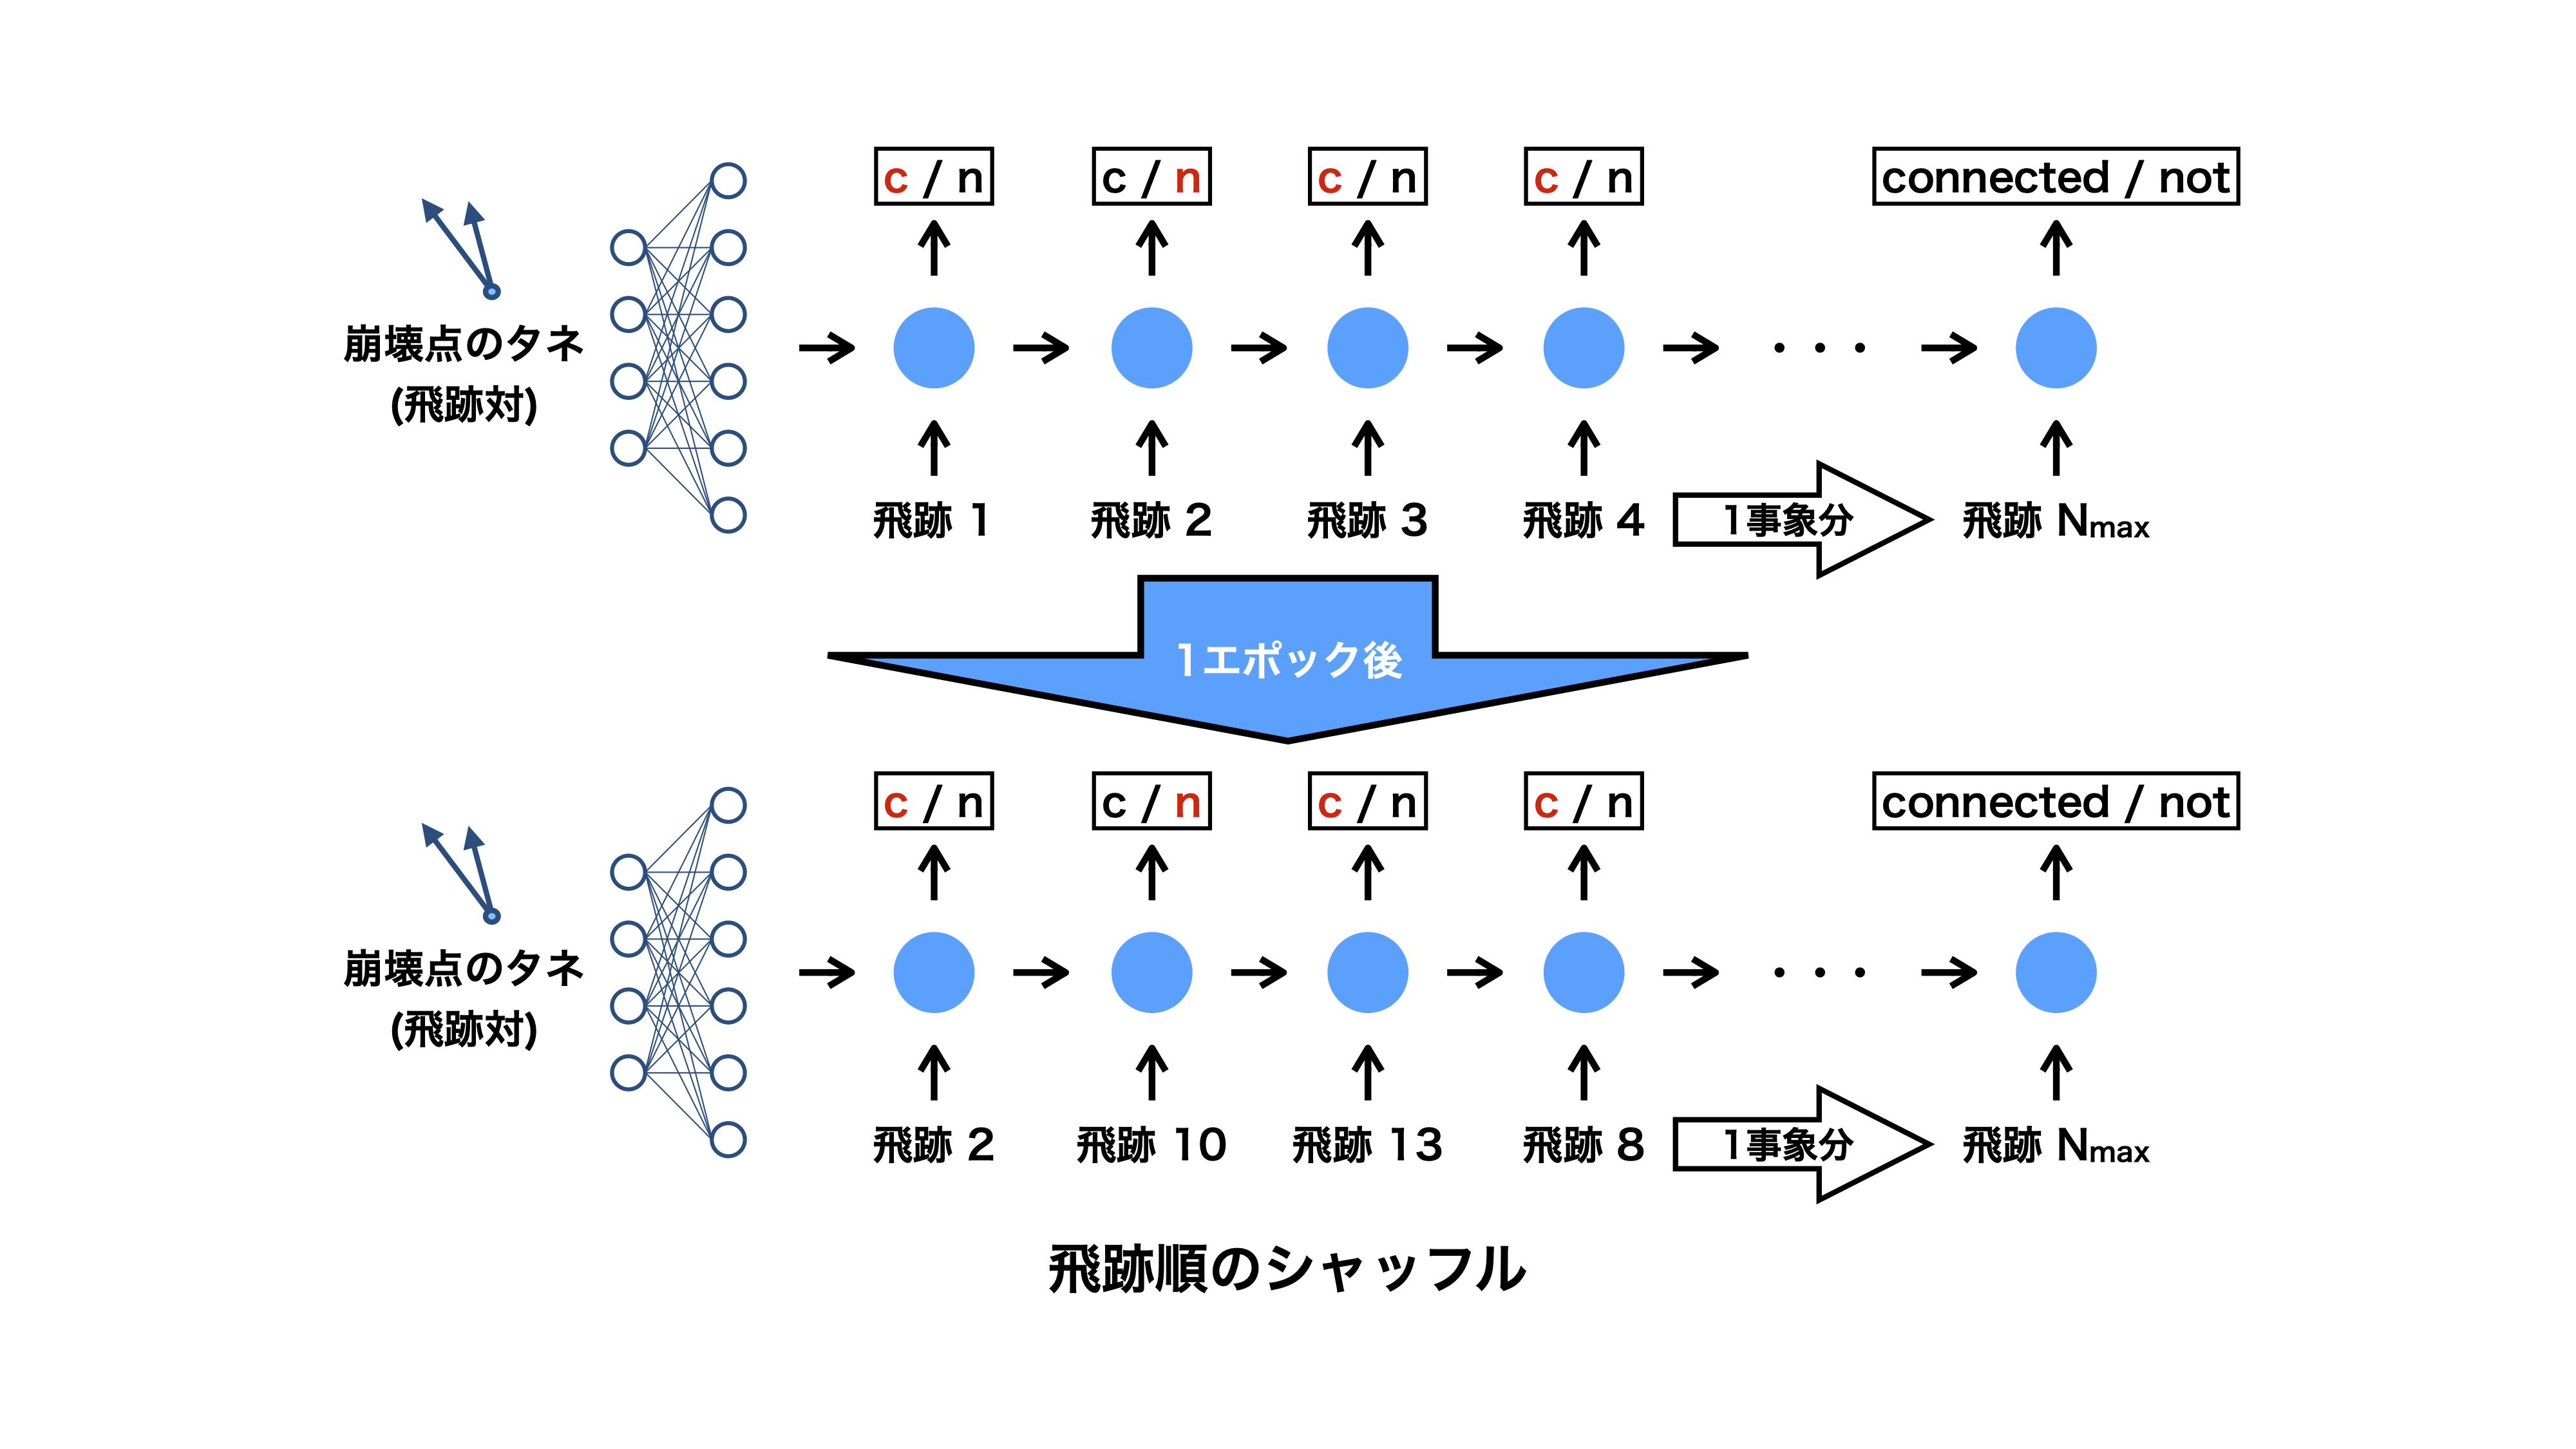
\includegraphics[trim = 150 50 150 0, width=0.9\textwidth, clip]{Figure/3Networks/3-4-2-1TrackShuffle.png}
 \caption{飛跡順のシャッフル}
 \label{3-4-2-1TrackShuffle}
\end{figure}

損失関数は二値交差エントロピー誤差を使用した。
ただし、前述したようにゼロ埋めした飛跡については損失関数や正答率の計算ではマスクした。
\begin{equation}
 \begin{split}
 L = -M_{\rm ZP}\ t_{\rm C} \log{(y_{\rm C})} - M_{\rm ZP}\ (1-t_{\rm C})\ \log{(1-y_{\rm C})}
 \end{split}
\end{equation}
$M_{\rm ZP}$はゼロ埋めのためのマスク変数 $(0, 1)$ である。

学習に使用したハイパーパラメータを表\ref{HyperparametersforVLSTMModel}に示す。
また、ネットワークの構造に使用したハイパーパラメータを表\ref{ParametersforVLSTMModel}に示す。

\begin{table}[htb]
 \centering
 \small
  \begin{tabular}{c c}\hline\hline
    最適化手法 & Adam\\
    学習率 & 0.001\\
    エポック数 & 100\\
    バッチサイズ & 32\\\hline\hline
  \end{tabular}
  \caption{任意の数の飛跡についてのネットワークで使用したハイパーパラメータ}
  \label{HyperparametersforVLSTMModel}
\end{table}

\begin{table}[htb]
 \centering
 \small
 \scalebox{0.8}{
  \begin{tabular}{l c c c}\hline
    層の名称 & 出力の形状 & パラメータ数 & 接続先\\\hline\hline
    Pair Input & (None, 44) & 0 & \\\hline
    Encoder Input & (None, 60, 23) & 0 \\\hline
    Decoder Input & (None, None, 23) & 0 \\\hline\hline
    Encoder Forward Dense 1 & (None, 256) & 11520 & Pair Input[0][0]\\\hline
    Encoder Backward Dense 1 & (None, 256) & 11520 & Pair Input[0][0]\\\hline
    Encoder Forward Activation 1 & (None, 256) & 0 & Encoder Forward Dense 1[0][0]\\\hline
    Encoder Backward Activation 1 & (None, 256) & 0 & Encoder Backward Dense 1[0][0]\\\hline
    Encoder Forward Dense 2 & (None, 256) & 11520 & Encoder Forward Activation 1[0][0]\\\hline
    Encoder Backward Dense 2 & (None, 256) & 11520 & Encoder Backward Activation 1[0][0]\\\hline
    Encoder Forward Activation 2 & (None, 256) & 0 & Encoder Forward Dense 2[0][0]\\\hline
    Encoder Backward Activation 2 & (None, 256) & 0 & Encoder Backward Dense 2[0][0]\\\hline\hline
    Encoder Embedding Dense & (None, 60, 256) & 6144 & Encoder Input[0][0]\\\hline\hline
    Bidirectional Encoder VLSTM & (None, 60, 512) & 1050624 & Encoder Embedding Dense[0][0]\\     
                                                                                                         &&&Encoder Forward Activation 2[0][0]\\       
                                                                                                         &&&Encoder Forward Activation 2[0][0]\\       
                                                                                                         &&&Encoder Backward Activation 2[0][0]\\     
                                                                                                         &&&Encoder Backward Activation 2[0][0]\\ \hline
    Reshape Bidirectional Encoder & (None, 27136) & 0 & Bidirectional Encoder VLSTM[0][0]\\\hline\hline
    Decoder Dense 1 & (None, 256) & 11520 & Pair Input[0][0]\\\hline
    Decoder Activation 1 & (None, 256) & 0 & Decoder Forward Dense 1[0][0]\\\hline
    Decoder Dense 2 & (None, 256) & 11520 & Decoder Forward Activation 1[0][0]\\\hline
    Decoder Activation 2 & (None, 256) & 0 & Decoder Forward Dense 2[0][0]\\\hline\hline
    Decoder Embedding Dense & (None, None, 256) & 6144 & Encoder Input[0][0]\\\hline\hline
    Decoder Attention VLSTM & (None, None, 1) & 1246976 & Decoder Embedding Dense[0][0]\\
                                                                                                   &&& Reshape Bidirectional Encoder[0][0]\\                    
                                                                                                   &&& Decoder Activation 2[0][0]\\\hline\hline
  \end{tabular}
  }
  \caption{任意の数の飛跡についてのネットワークにおける訓練可能なパラメータ}
  \label{ParametersforVLSTMModel}
\end{table}

エポック数を横軸に、正答率と損失を縦軸にプロットした学習曲線を図\ref{3-4-2-2TrainingCurve}に示す。

%\begin{figure}[htbp]
 %\centering
 %\includegraphics[width=1.0\textwidth]{Figure/3Networks/3-4-3-2TrainingCurve.png}
 %\caption{任意の数の飛跡についてのネットワークの学習曲線}
 %\label{3-4-3-2TrainingCurve}
%\end{figure}


%%%%%%%%%%%%%%%%%%%%%%%%%%%%%%%%%%%%%%%%%%%%%%%%%%%%%%%%%%%%%%%%%%%%%%%%
\subsection{ネットワークの性能} \label{Net:VLSTM:PerformanceofVLSTM}

コンテキストを含めて変わるか否か\\
VLSTM SimpleとEncoder-Decoderの比較 ROCカーブ\\

Attention weight\\
Connectedな飛跡を見ているか (ぬまりそうならある程度で見切りをつける)\\
PrimaryとSecondaryの差があるか\\
Attentionされている飛跡に何か傾向があるか\\

Primary, Secondary, 終状態bb, cc\\
に特化すれば性能は上がるか ROCカーブ\\









